
\section{Software Requirements Specification}

\vspace{20mm}



\begin{abstract}
	In this chapter,we will discuss a software development process which is generally consists of several stages ranging from analysis
    to implementation, which will result in need (requirement) of software. Results of analysis for different
    applications in a similar problem domain will usually produce similar definition needs. In the field of 
    software engineering, especially in object- oriented software development, requirements for different problem
    domain have been developed. This research is to obtain a similarity (commonality) of the software requirements
    specifications, here in after in short-SRS. Management Information System (MIS) has been chosen due to several
    years has developed into concepts that are essential both in the scope of major agencies as well as small and medium
    scale. SRS is the identification of commonality for the MIS application which is focused on the function of customer
    service standards, particularly for the Management Information System. From this research it also can be concluded
    that the SRS commonality can be generated by capturing best practices from existing business processes.
    
\end{abstract}

\vspace{20mm}

\large{\textbf{Outline}}

\begin{center}
    \begin{itemize}
        \item Introduction
              \begin{itemize}
                  \item Purpose
                  \item Scope
              \end{itemize}
        \item Overall Description
        \item User Characteristics
        \item Specific Requirements
              \begin{itemize}
                  \item Functional Requirements
                  \item Non-Functional Requirements
              \end{itemize}
    \end{itemize}
\end{center}
\pagebreak


\subsection{Introduction}

A software requirements specification SRS describes all the requirements system which must-have for success.
These requirements are typically illustrating features of an underdevelopment system. These features not only
describe its functional requirements FR but also its nonfunctional requirements NFR. Functional requirements
as well nonfunctional requirements are equally significant for successful development. Both FR and NFR have
an impact on the overall success of any system. In contrast to FRs which are described deliberately in SRS,
NFRs are not described explicitly. If some NFRs are described deliberately, there are multiple NFRs implicitly
defined hidden in plain text. Encoding software requirements from the earliest period of development are 
more focused on functional requirements.

\hspace{10mm}Non-functional requirements either neglected or described as a whole
i.e., not for the individual design problem. These requirements artifacts are encoded without any prescribed
standards, it can be either structured, semi-structured, or completely unstructured. To learn
these non-functional requirements, we have to understand the genre of requirements artifacts are organized 
such as Modules, submodules, and finally atomic design problems. These design problems are not defined in any
structured way most of the time requirement encoders spent more time on functional requirements. These 
requirements in a textual form commonly describe functional requirements, however, implicitly define non-functional
requirements as well. The textual data for requirement extraction can be used for the extraction of underlying functional
requirements. To learn these underlying functional requirements a standardized way of encoding, functional
requirements must be developed. Requirements artifacts are encoded using the wording of end-users i.e. interviews 
or the words of requirement from requirement inceptor i.e. owner, end-users.


 \subsection{Purpose}
 Software requirement artifacts such as manuals request for proposals, and software requirements specification (SRS) are
 commonly focused on functional requirements. In most SRS files, nonfunctional requirements do not formally encoded or 
 encoded as a whole, not for an individual design problem. Moreover, these nonfunctional requirements are intermingled 
 with functional requirements. Therefore, these nonfunctional requirements need special attention to understand for
 successful project development. These nonfunctional requirements have an impact on each other and optimal tradeoff is
 required for balanced nonfunctional requirements set. NFRs have a negative and positive tradeoff with each other such
 as increase confidentiality, decrease the availability, and enhance authenticity.So, an optimum tradeoff among these 
 design problem within a module is required to have better design decisions. 
 
 \hspace{10mm}Instead of considering all nonfunctional
 requirements, the NFRs that have mutual tradeoff is considered. In this paper, we devised a novel document annotation
 scheme for SRS and extracted nonfunctional requirements from these annotated artifacts. In the next step, we classified
 NFRs into two classes security triad and performance triad, and the cost is assumed constant for each NFR. From the design
 problem, the tradeoff ratio is calculated among NFRs associated with it. Then, the production possibility graph is plotted
 to estimate the optimum tradeoff ratio within the module. For estimation economic optimum from a set of NFR, iso-cost graphs
 by assuming the constant cost. Some hypothetical variations in cost are also examined using 3D iso-cost graph. The reason to
 measure these tradeoff is to make design decision more empirical and helpful for the selection of design patterns, especially
 secure design patterns.

    \subsection{Product Scope}
    The major Scope of our Project is to estimate the actual cost of the project and helpful to managers of the software industry
    are likely easy to calculate the budget of the developing software, and also easy to assign the developer to the particular 
    developing software. This application helps Software Associations for dealing with an upcoming project in terms of their cost 
    as well as effort applied for that project. So they easily decide that they have to work on that project or not as well as they also
    know that either they have the developer of that technology or not so they recruited that type of programmers.
    \\
    
    \subsubsection{Definition acronym \& abbrevation}
    The following acronym are used in our documents
    \begin{center}
        \begin{itemize}
            \item {\bfseries MERN:} MongoDB ExpressJS ReactJS NodeJS
            \item {\bfseries REST:} Restfull
            \item {\bfseries API:} Application Programming Interface
            \item {\bfseries DB:} Database
            \item {\bfseries SRS:} Software Requirements Specification
            \item {\bfseries UCP:} Use Case Point
            \item {\bfseries SPA:} Single Page Application
            \item {\bfseries CBR:} Content Base Reasoning
            \item {\bfseries FRs:} Functional Requirements
            \item {\bfseries NFRs:} Non-Functional Requirements
            \end{itemize}
    \end{center}
    
\subsection{Overall Description}
\subsubsection{Product Perspective}
Our Final Year Project is SPA(Single Page Application). To reduce the difficulties for those managers who feels 
difficulties to estimate the actual effort/cost of the upcoming project. Managers can also some other modules except
the Estimation i.e {\bfseries View/Update project} and {\bfseries Add/Remove Developers} in a project. Other than manager, there is a developer module in which developer 
can View and inform estimation of the project. Manager also have option to use our all methods for estimation as well as choose only one or two for calculating the actual estimate of the project.

    \subsubsection{System Interfaces:}
    Our Proposed system is built from the scratch from the modern technology and add one feature from the exciting application. 
    \subsubsection{User interface: }
    The interface of the website is designed to be simple and interactive and be Single Page Application to improve the user experience. 
    For attracting the developer and managers, we have facilitate them to change the theme of the system as they can feel to easy for work.
    As we know who attract with our system has well knowledge of how to operate a website but we kept as easy to operatable.
    \subsubsection{Hardware Interfaces}
    The website can be used on any device such as a mobile phone laptop, computer or a tab as long as it has active Internet connection.
    \subsubsection{Software Interface}
    Software interfaces include operating system for the computer, a browser to access the website with internet connectivity.
    \subsubsection{Prototype}
    \begin{figure}[H]
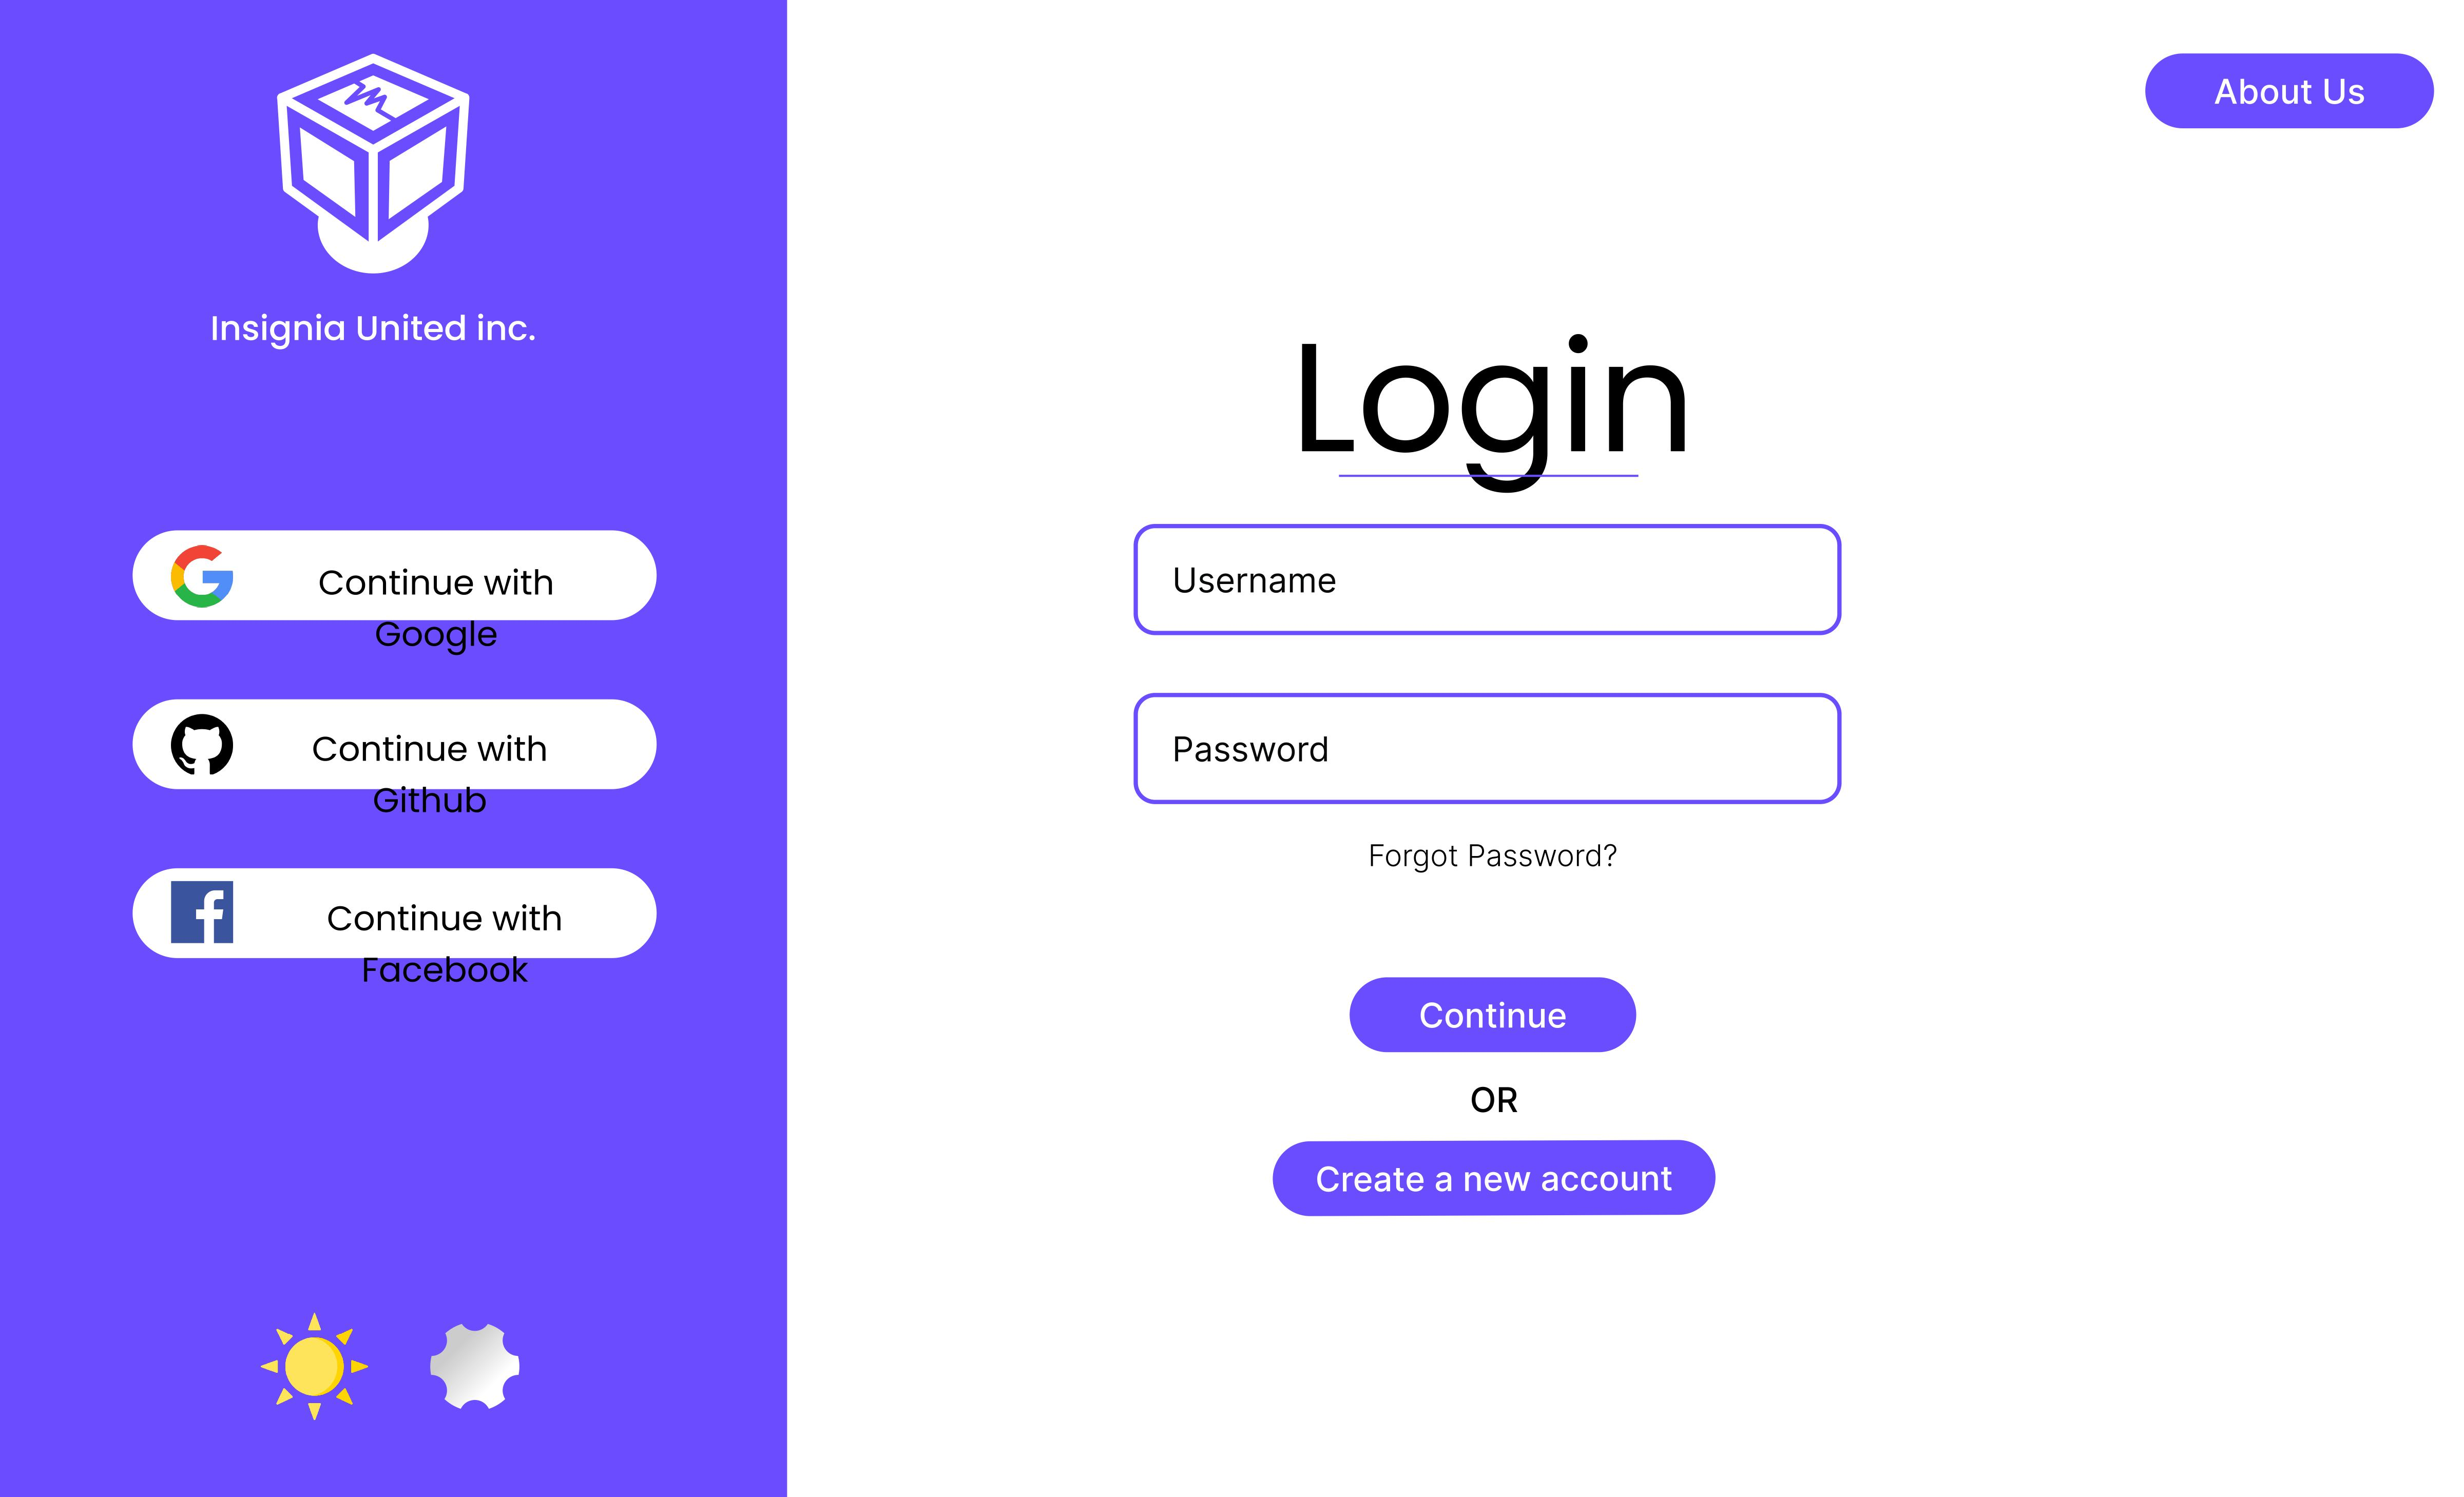
\includegraphics[height=10cm, width=1\textwidth]{./images/prototype/0001}
 \caption{Login Page}
\label{fig:prototype1} 

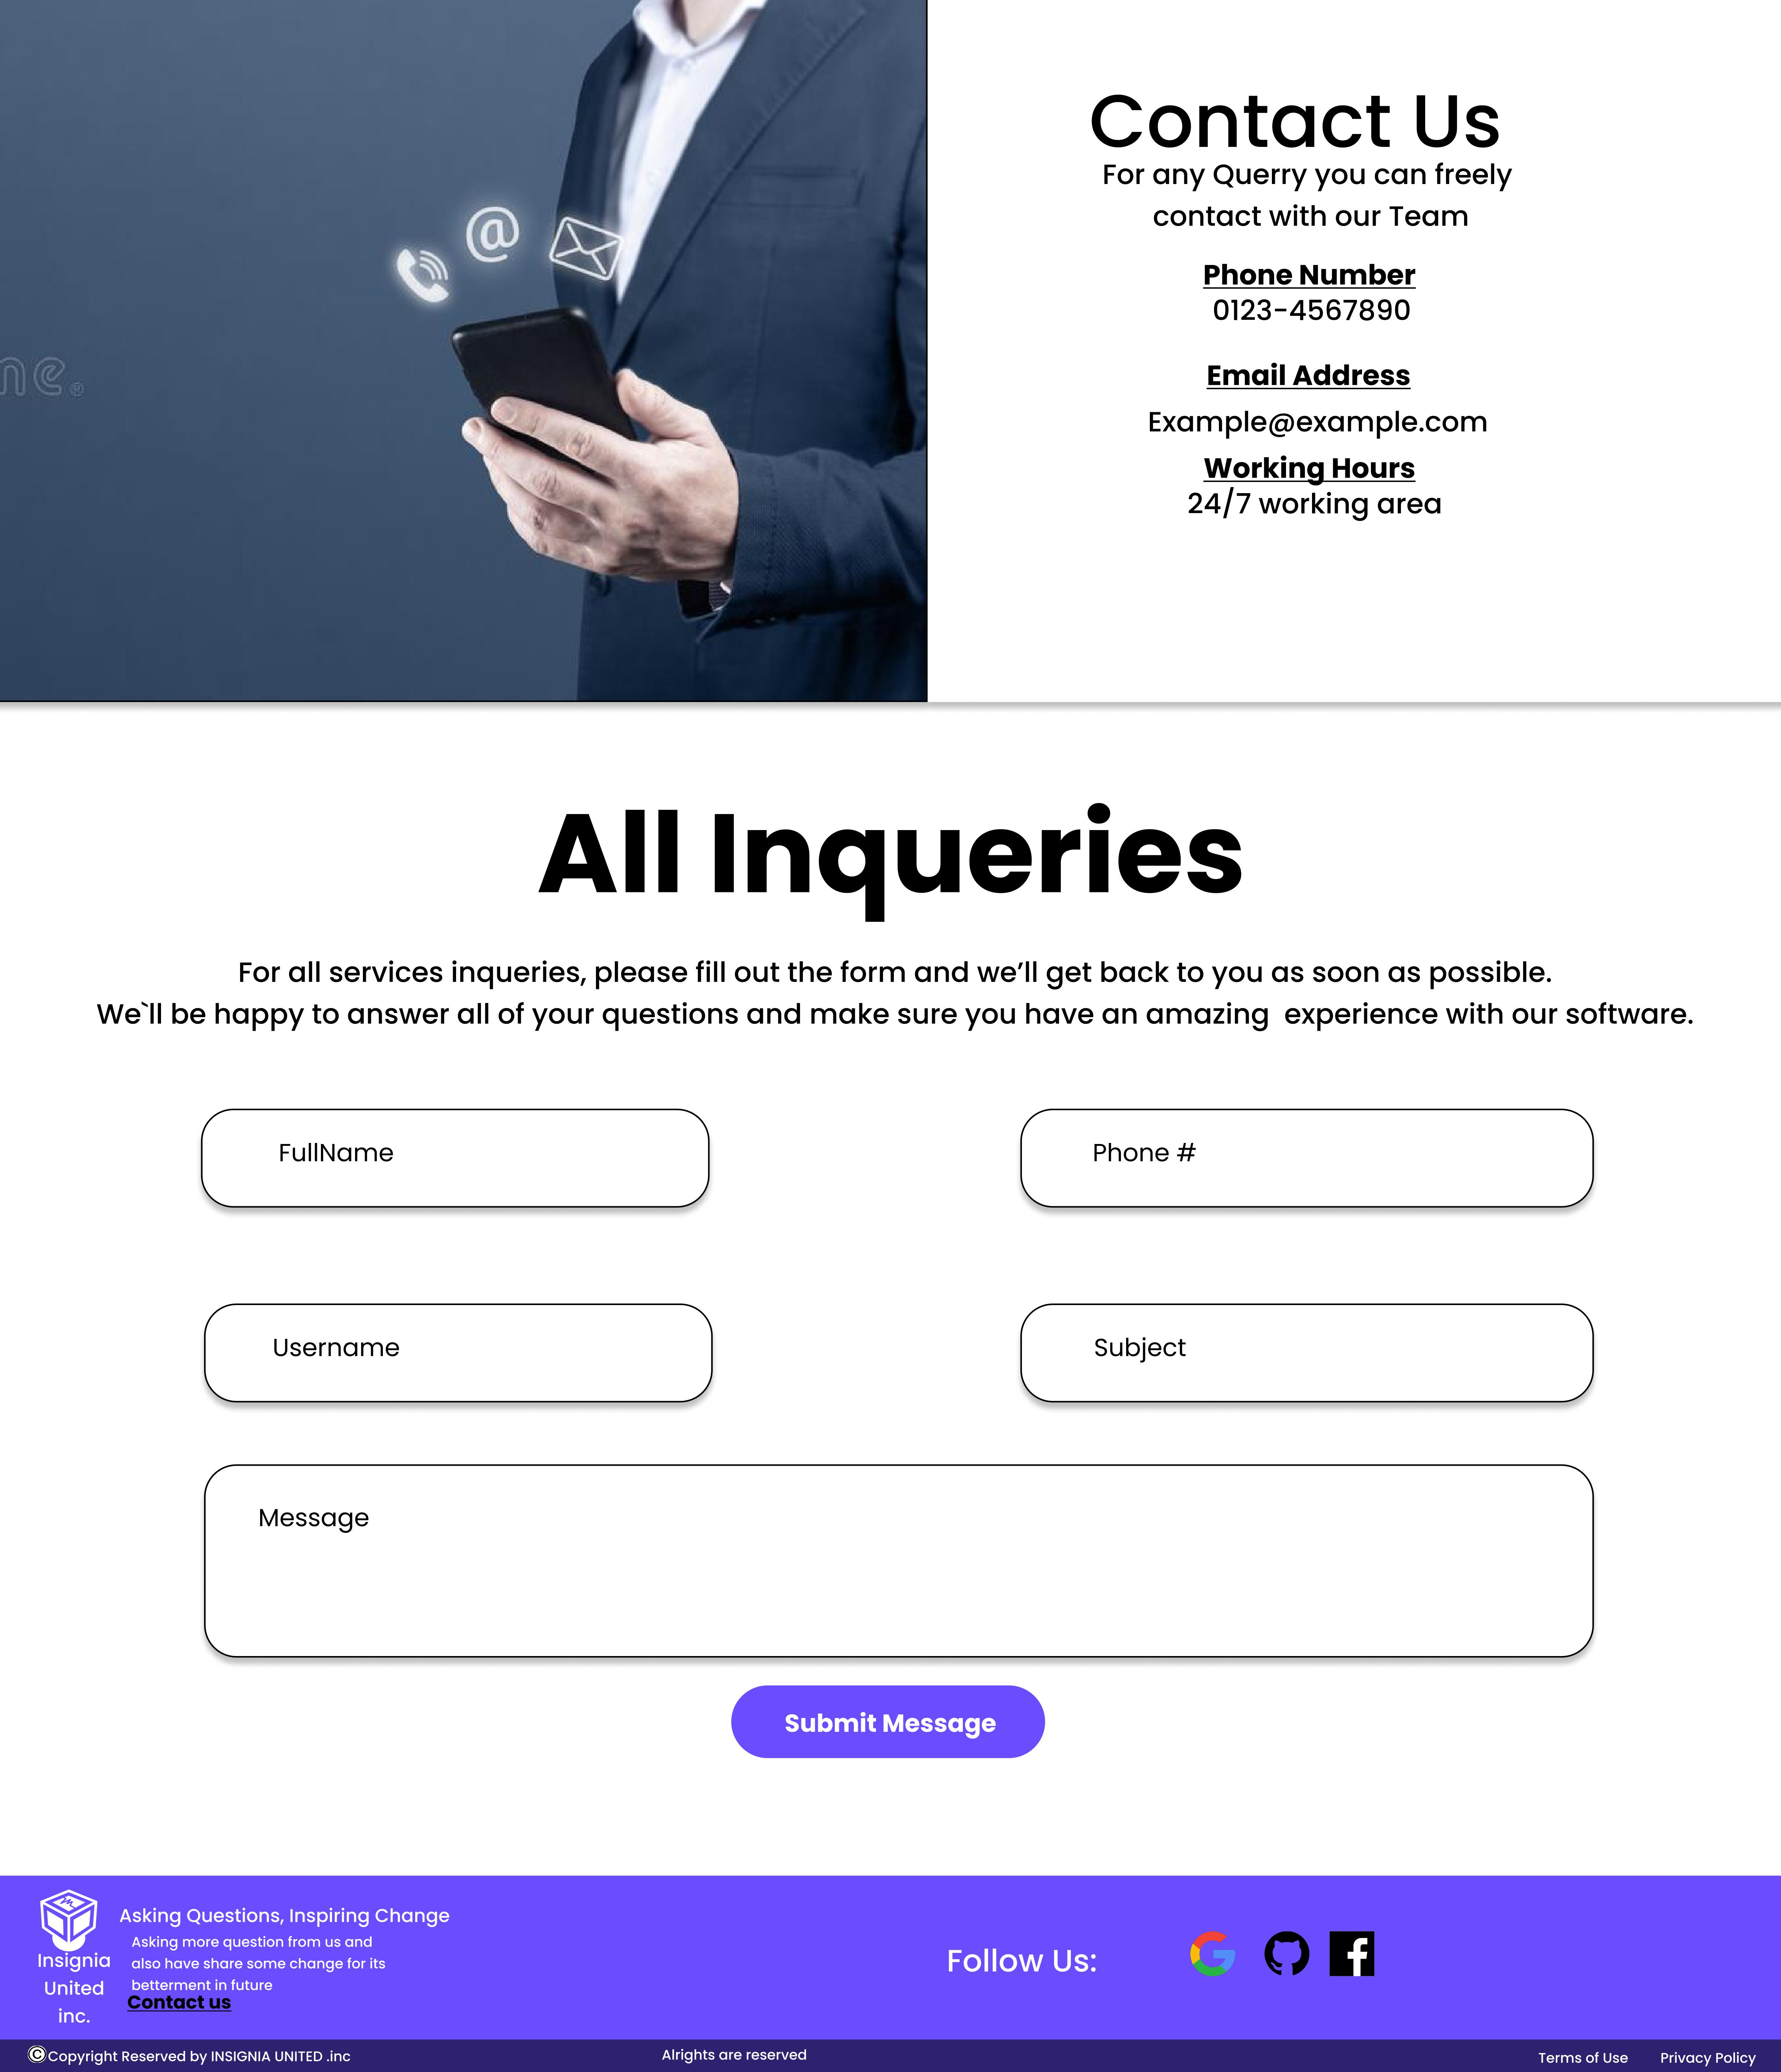
\includegraphics[height=12cm, width=0.9\textwidth]{./images/prototype/0002}
\centering 
\caption{Login Page}
\label{fig:prototype1}
\end{figure}

\begin{figure}[H]
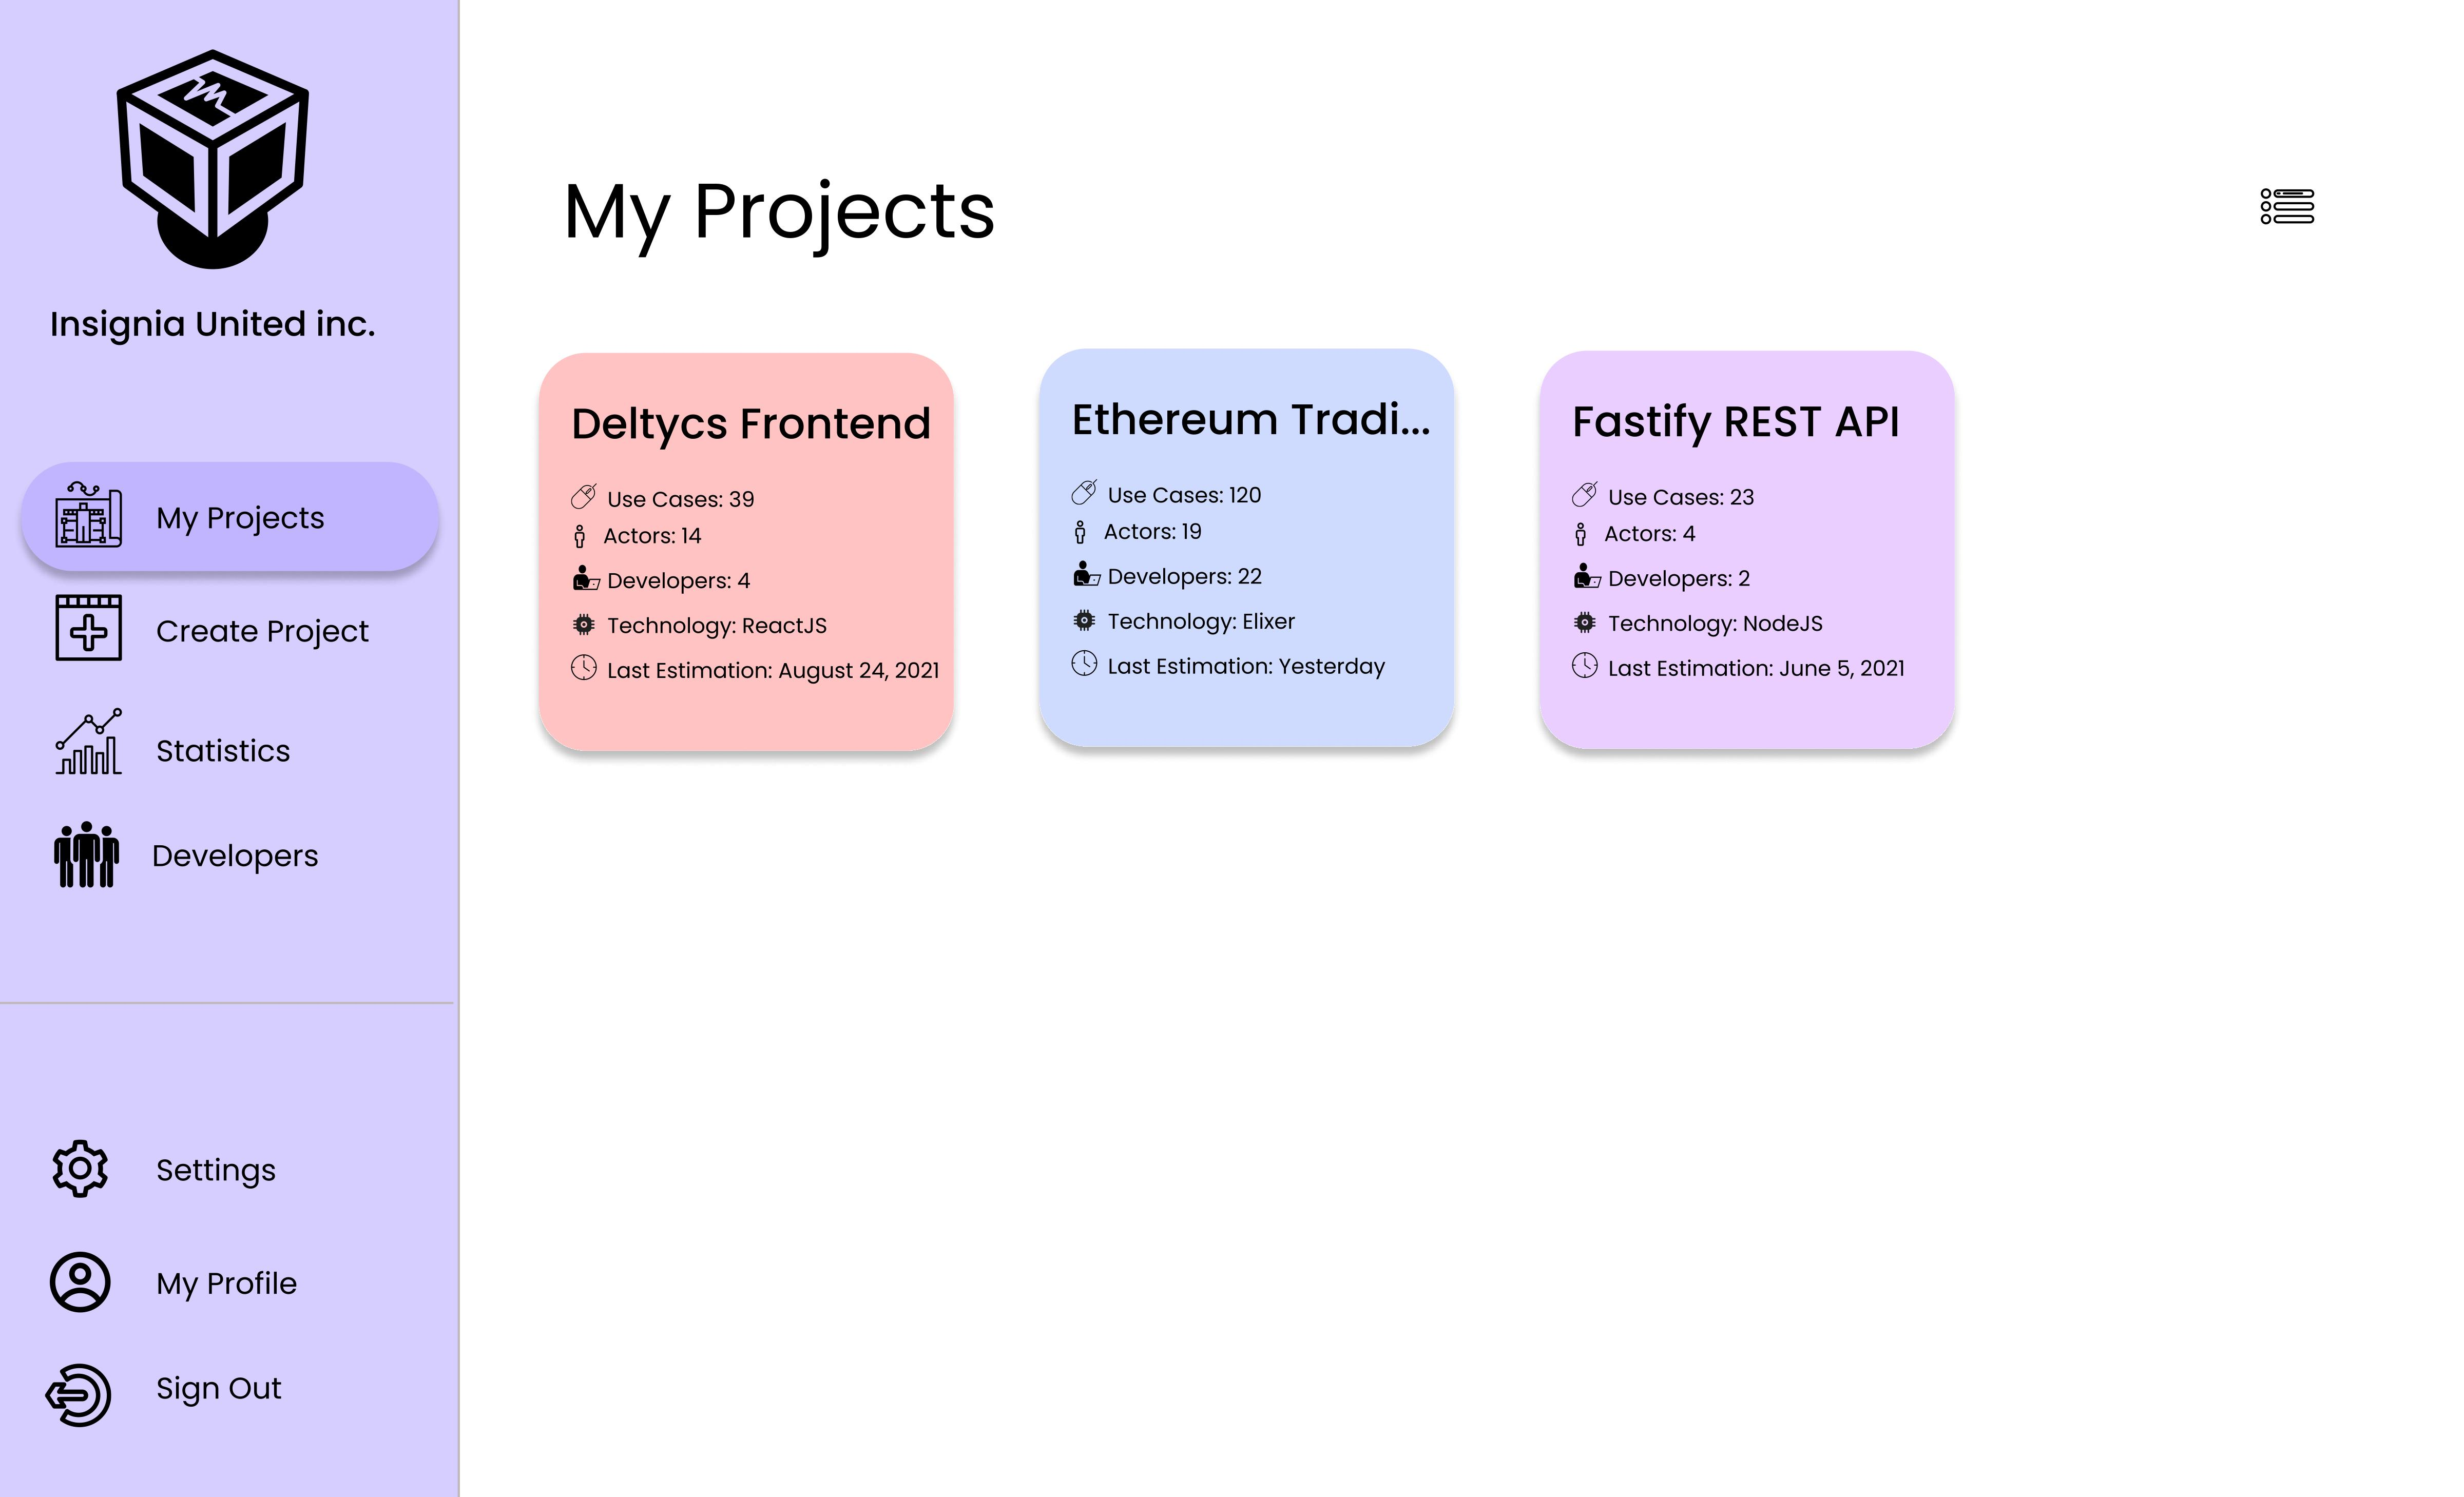
\includegraphics[height=10cm, width=0.9\textwidth]{./images/prototype/0003}
\centering 
\caption{Login Page}
\label{fig:prototype1}

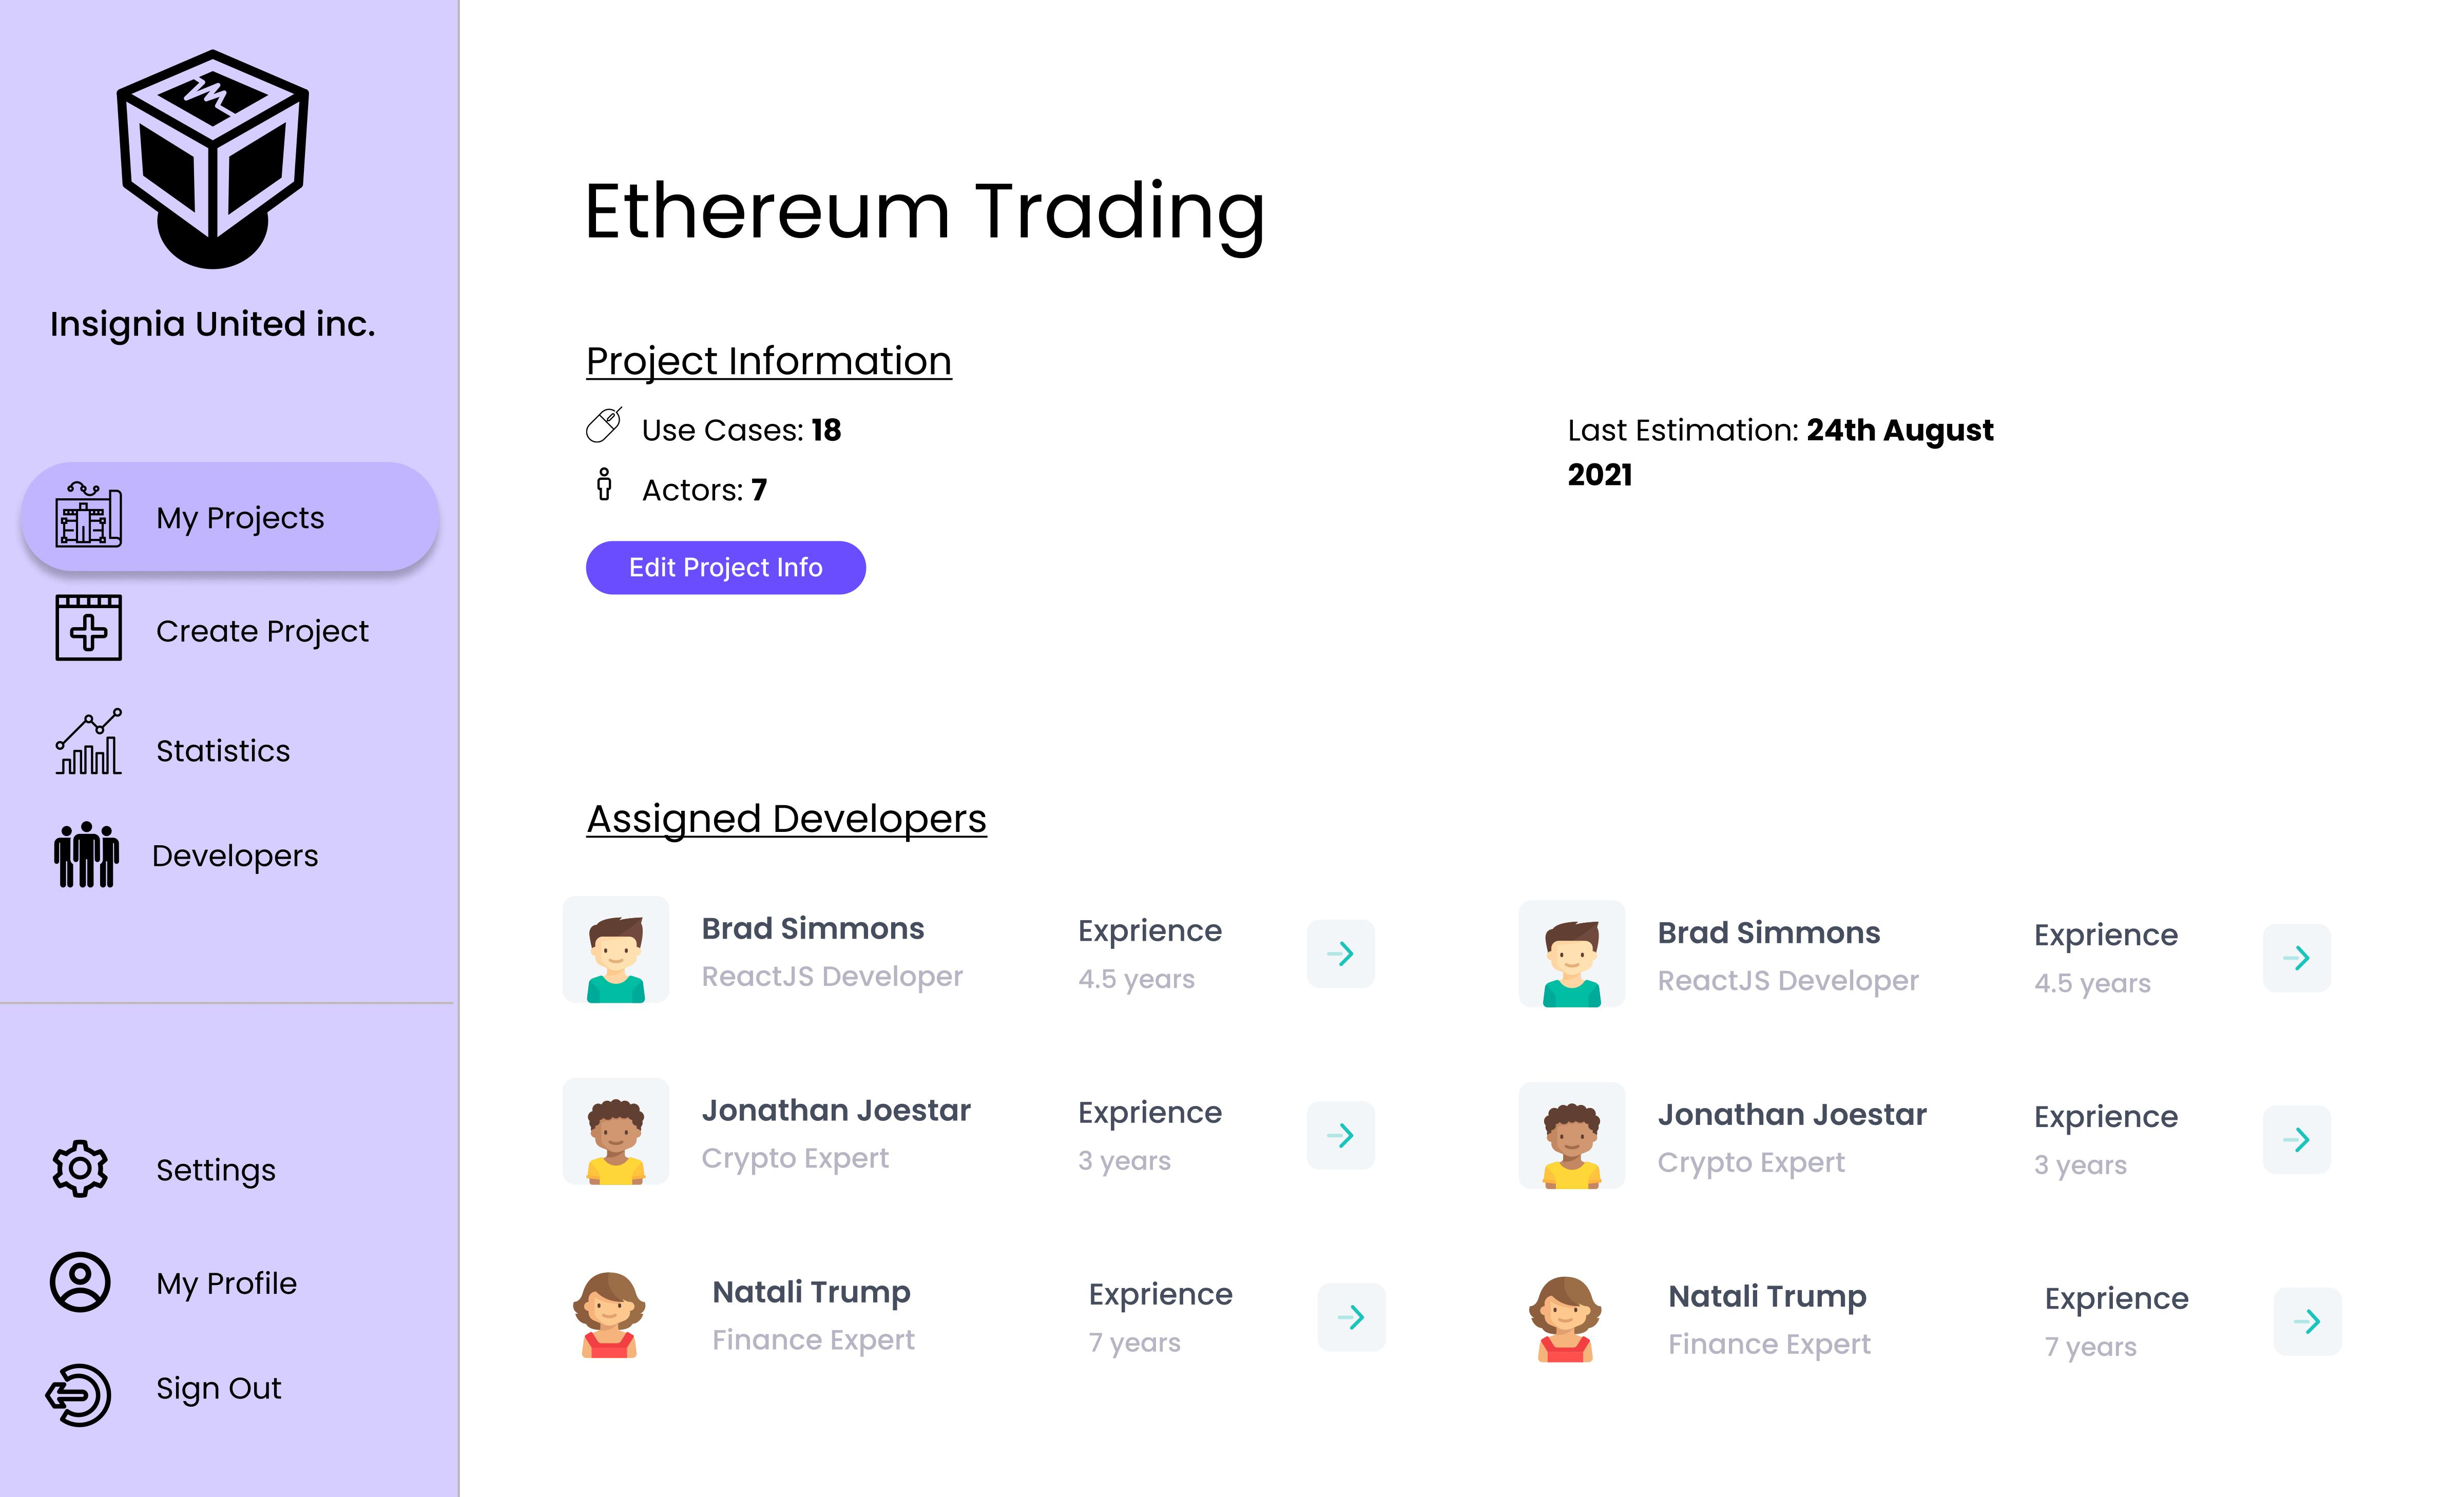
\includegraphics[height=10cm, width=0.9\textwidth]{./images/prototype/0004}
\centering 
\caption{Login Page}
\label{fig:prototype1}
\end{figure}

\begin{figure}[H]
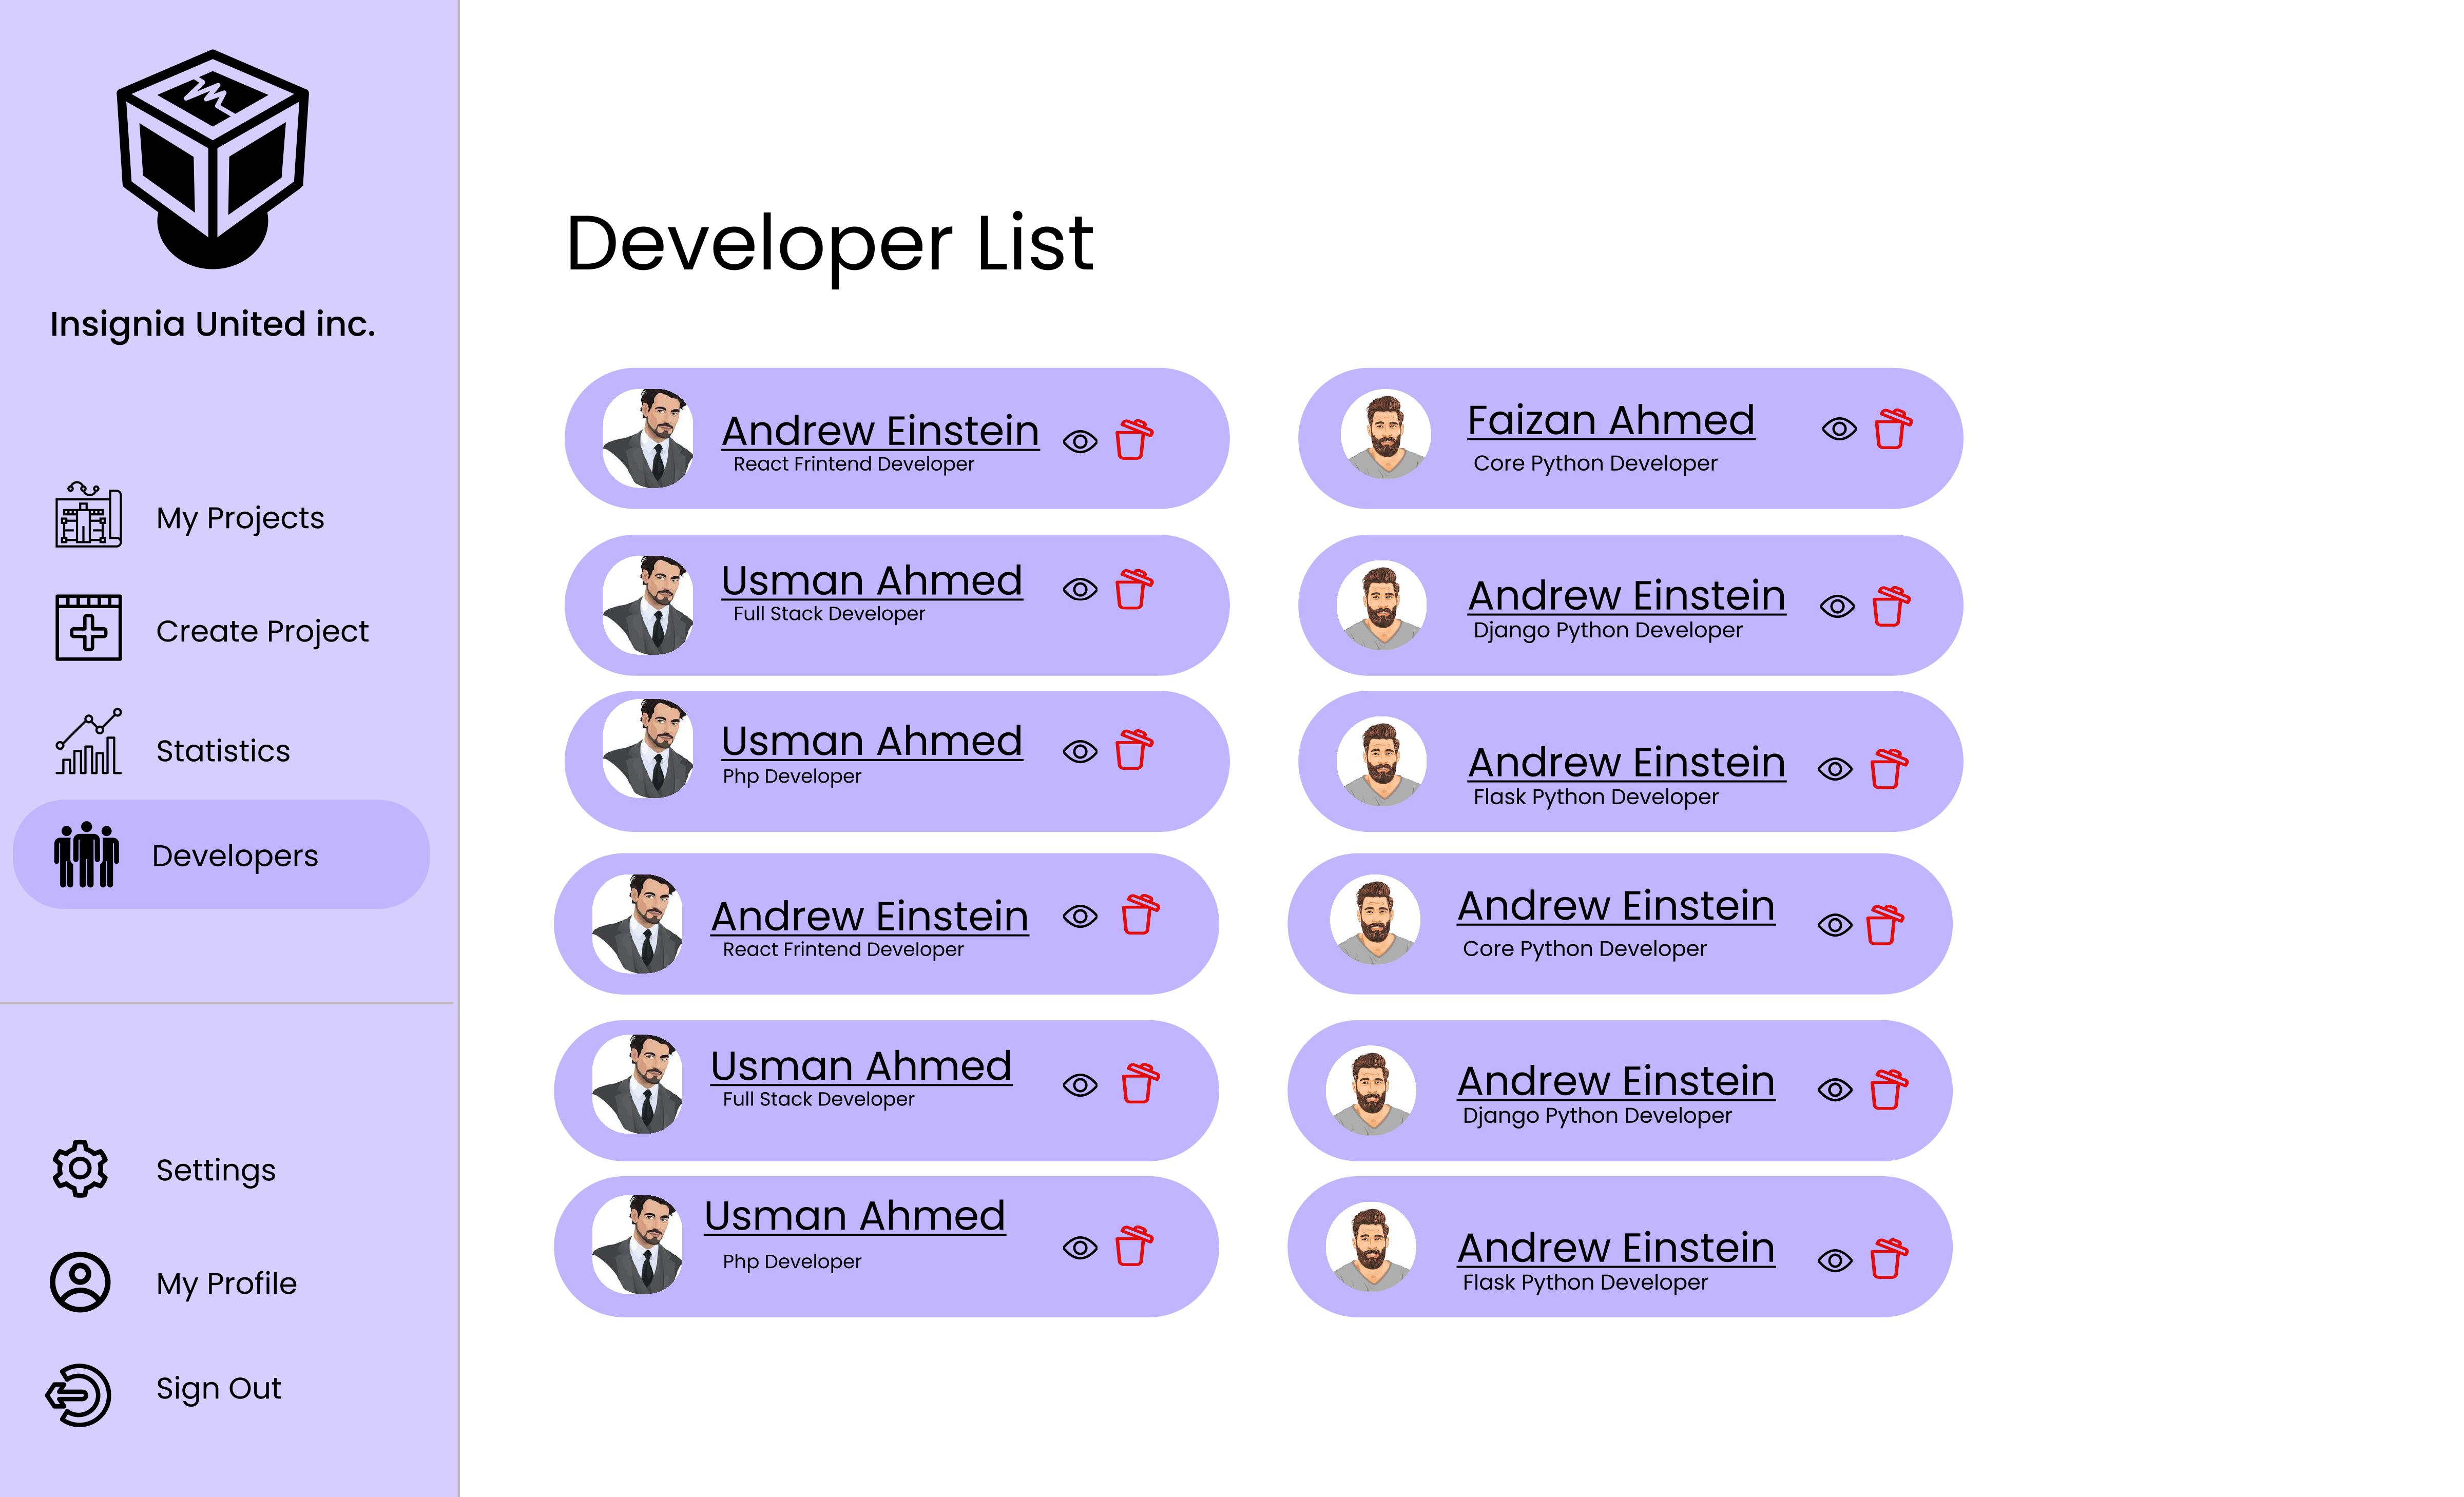
\includegraphics[height=10cm, width=0.9\textwidth]{./images/prototype/0005}
\centering 
\caption{Login Page}
\label{fig:prototype1}

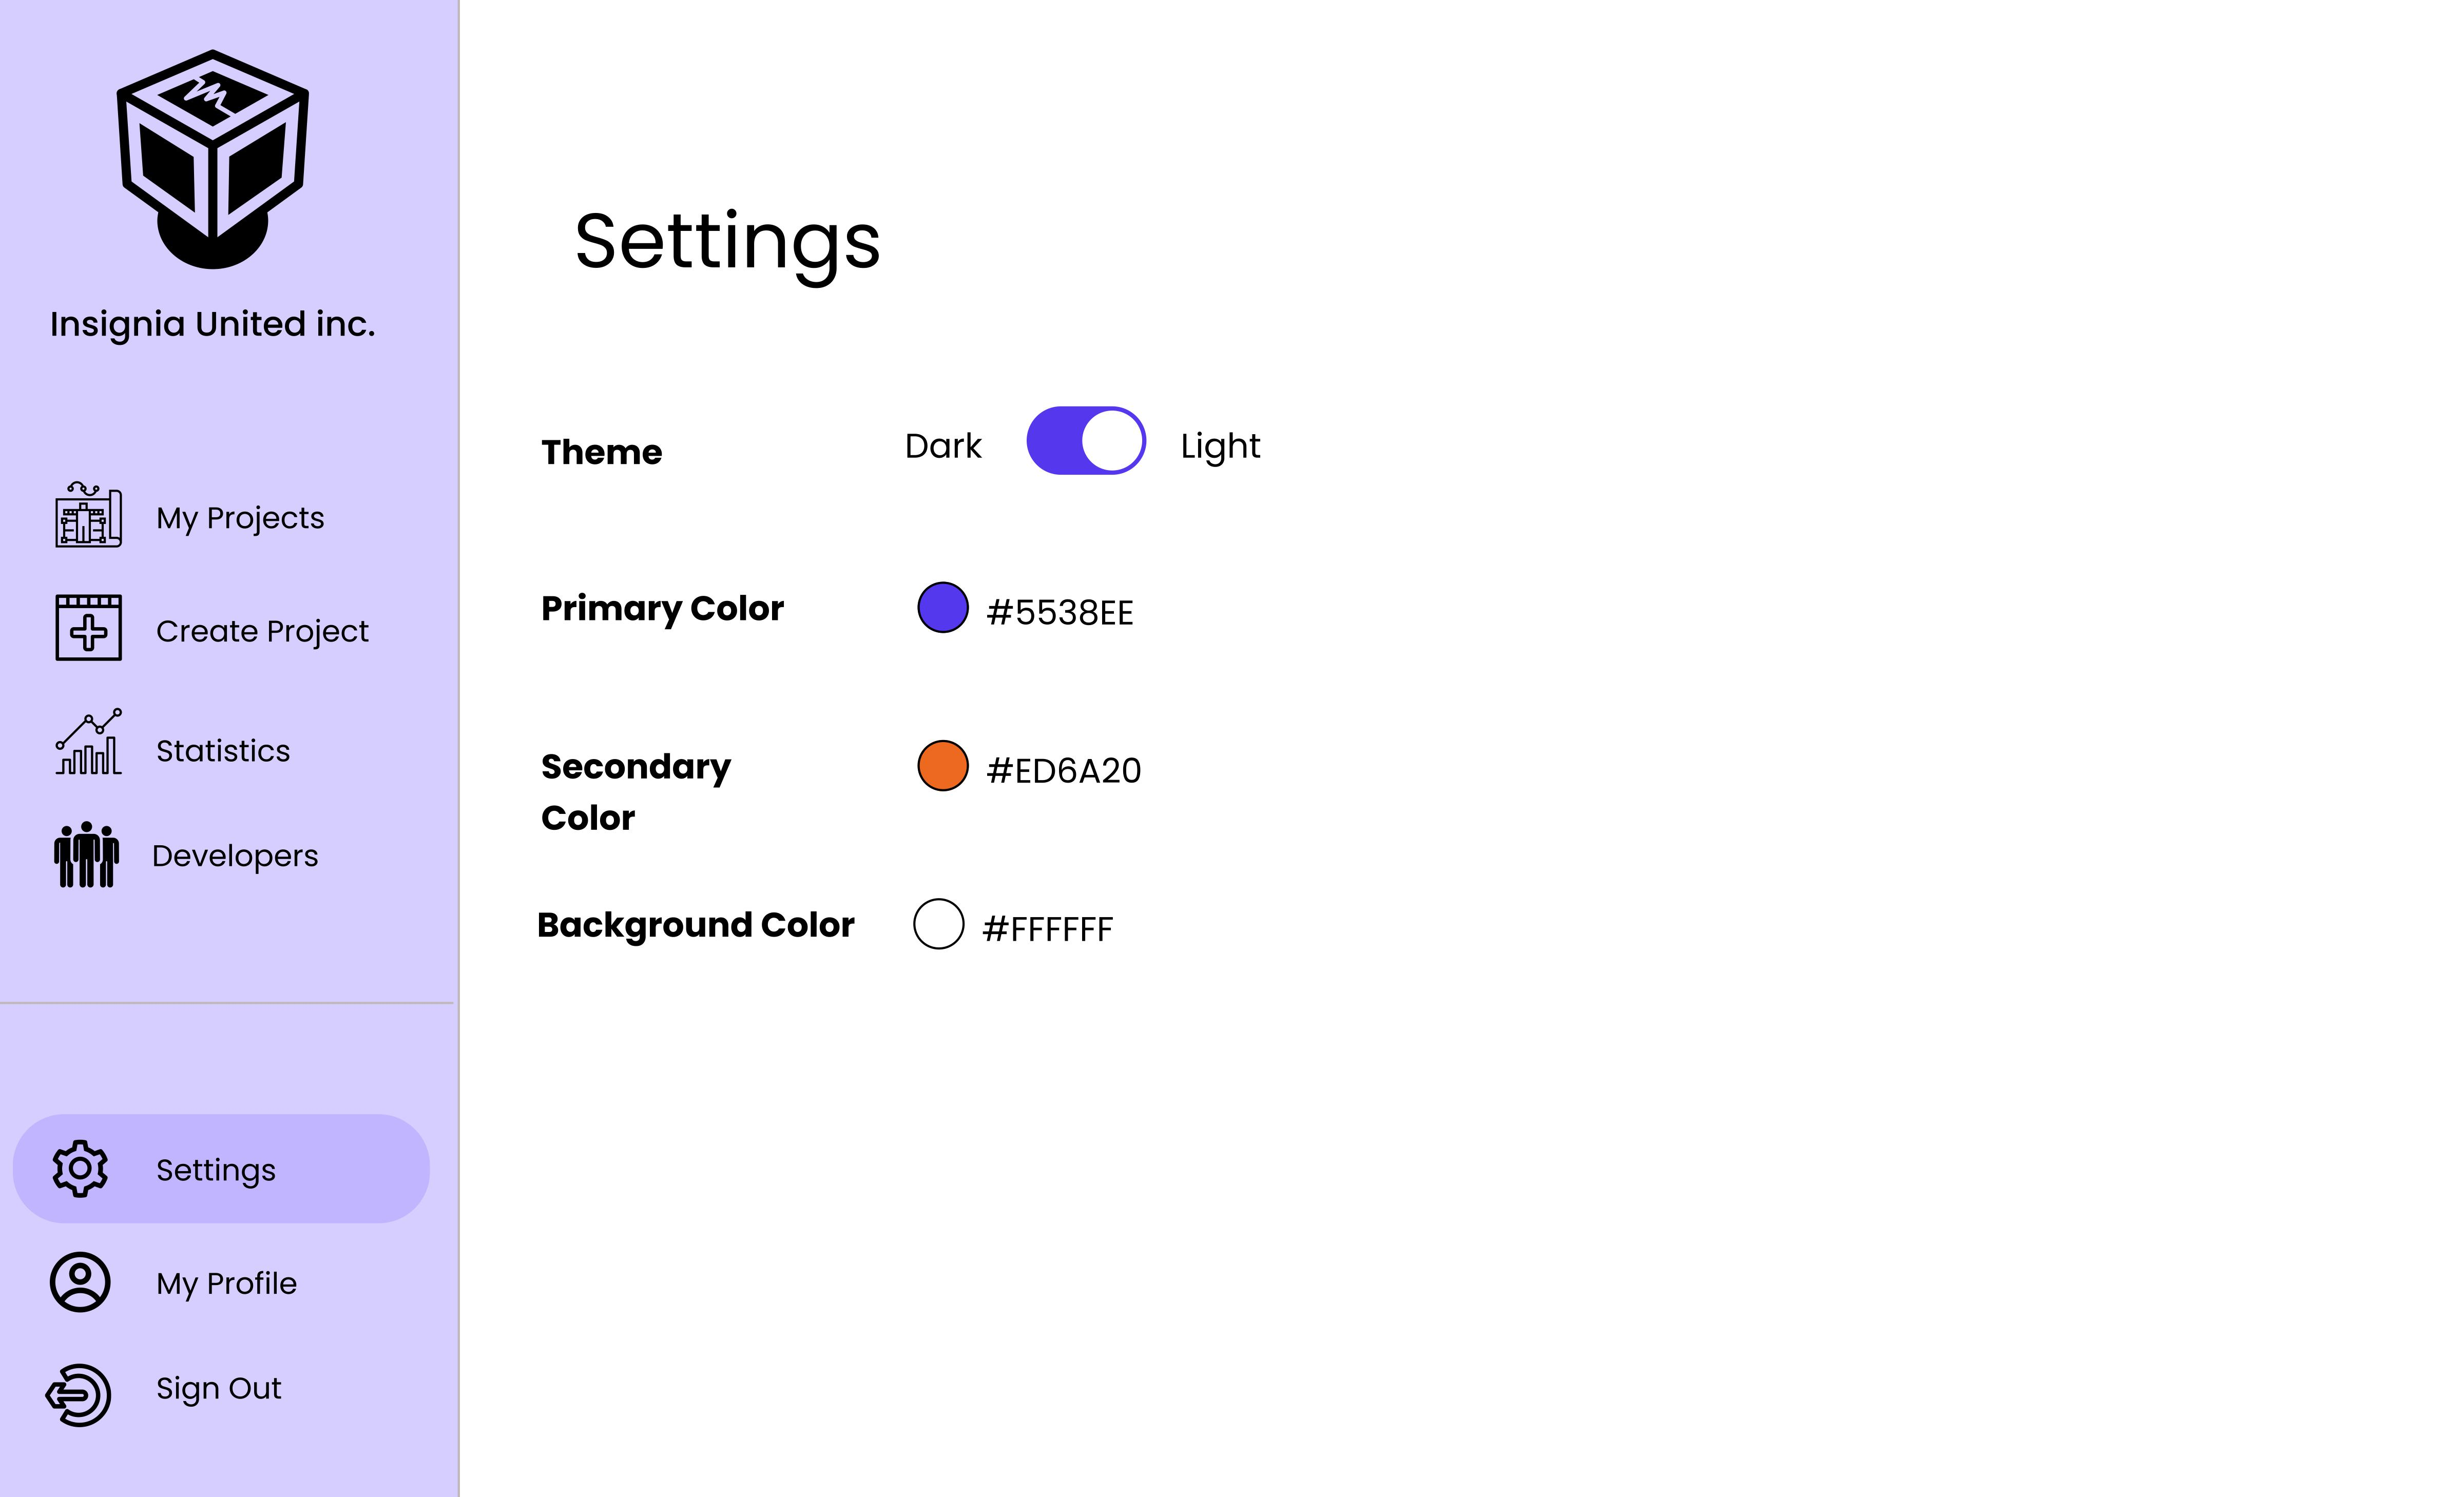
\includegraphics[height=10cm, width=0.9\textwidth]{./images/prototype/0006}
\centering 
\caption{Login Page}
\label{fig:prototype1}
\end{figure}

\begin{figure}[H]
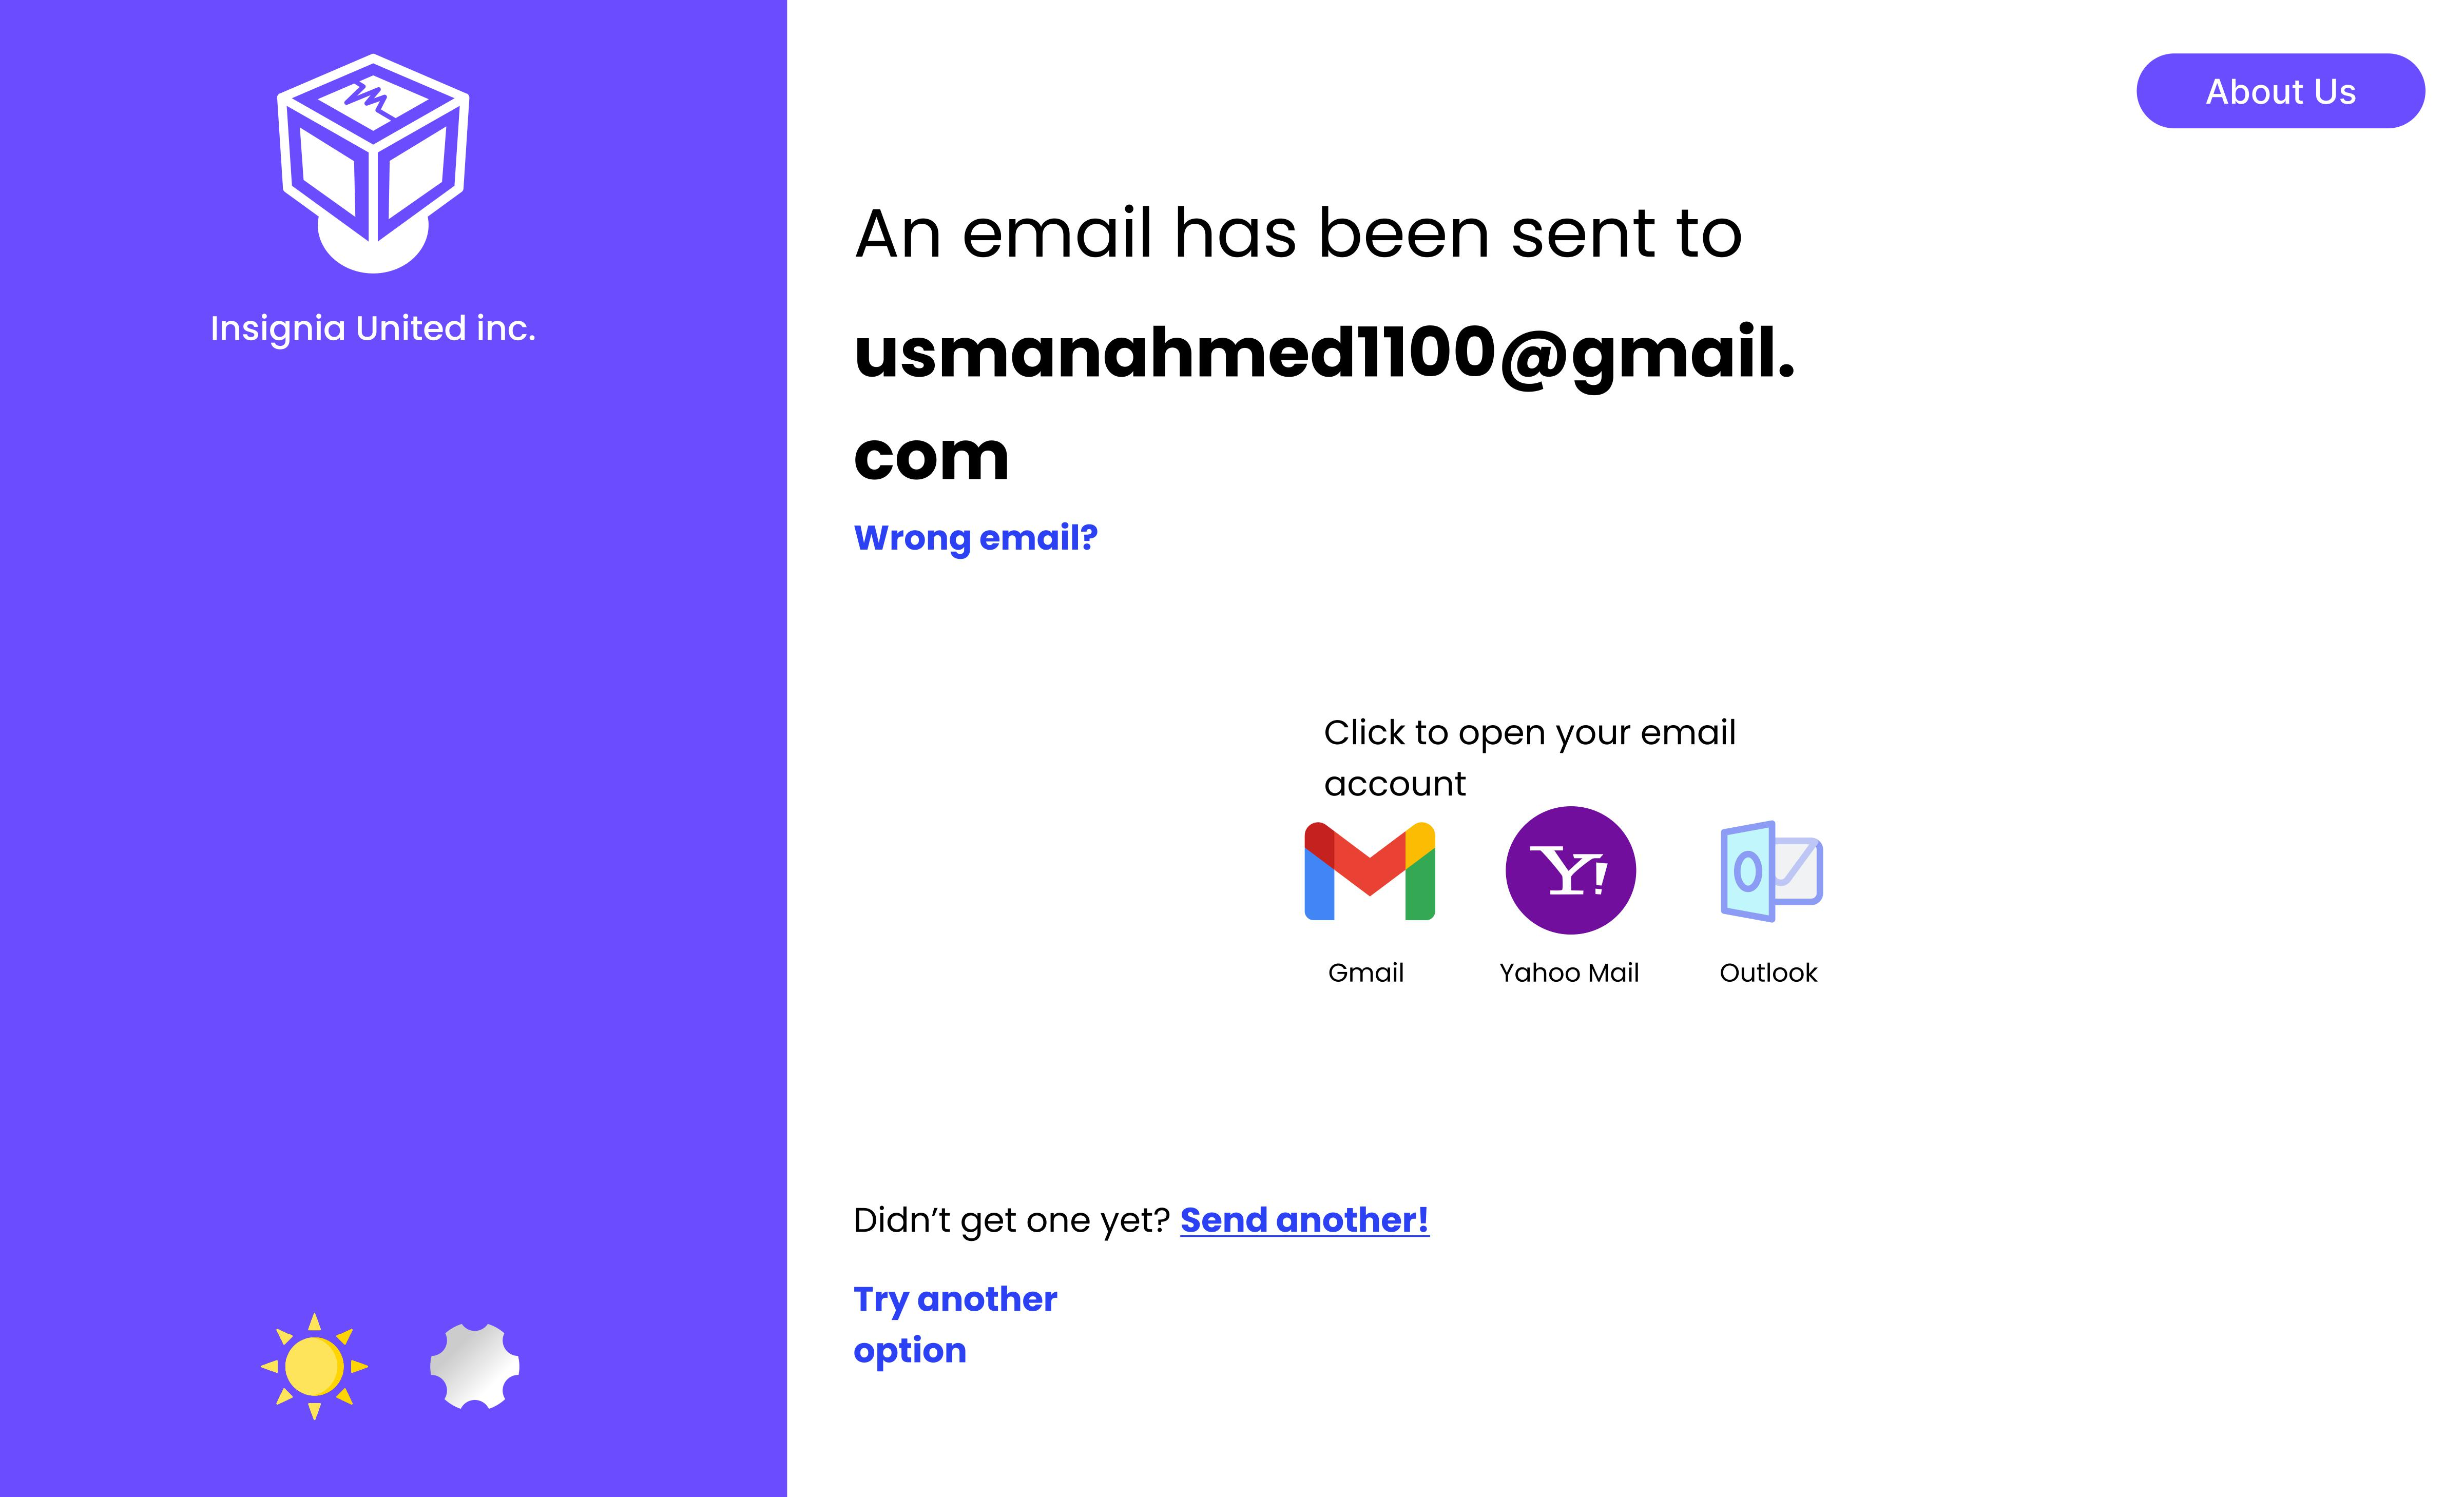
\includegraphics[height=10cm, width=0.9\textwidth]{./images/prototype/0007}
\centering 
\caption{Login Page}
\label{fig:prototype1}


\includegraphics[height=10cm, width=0.9\textwidth]{./images/prototype/0008}
\centering 
\caption{Login Page}
\label{fig:prototype1}
\end{figure}

\begin{figure}[H]
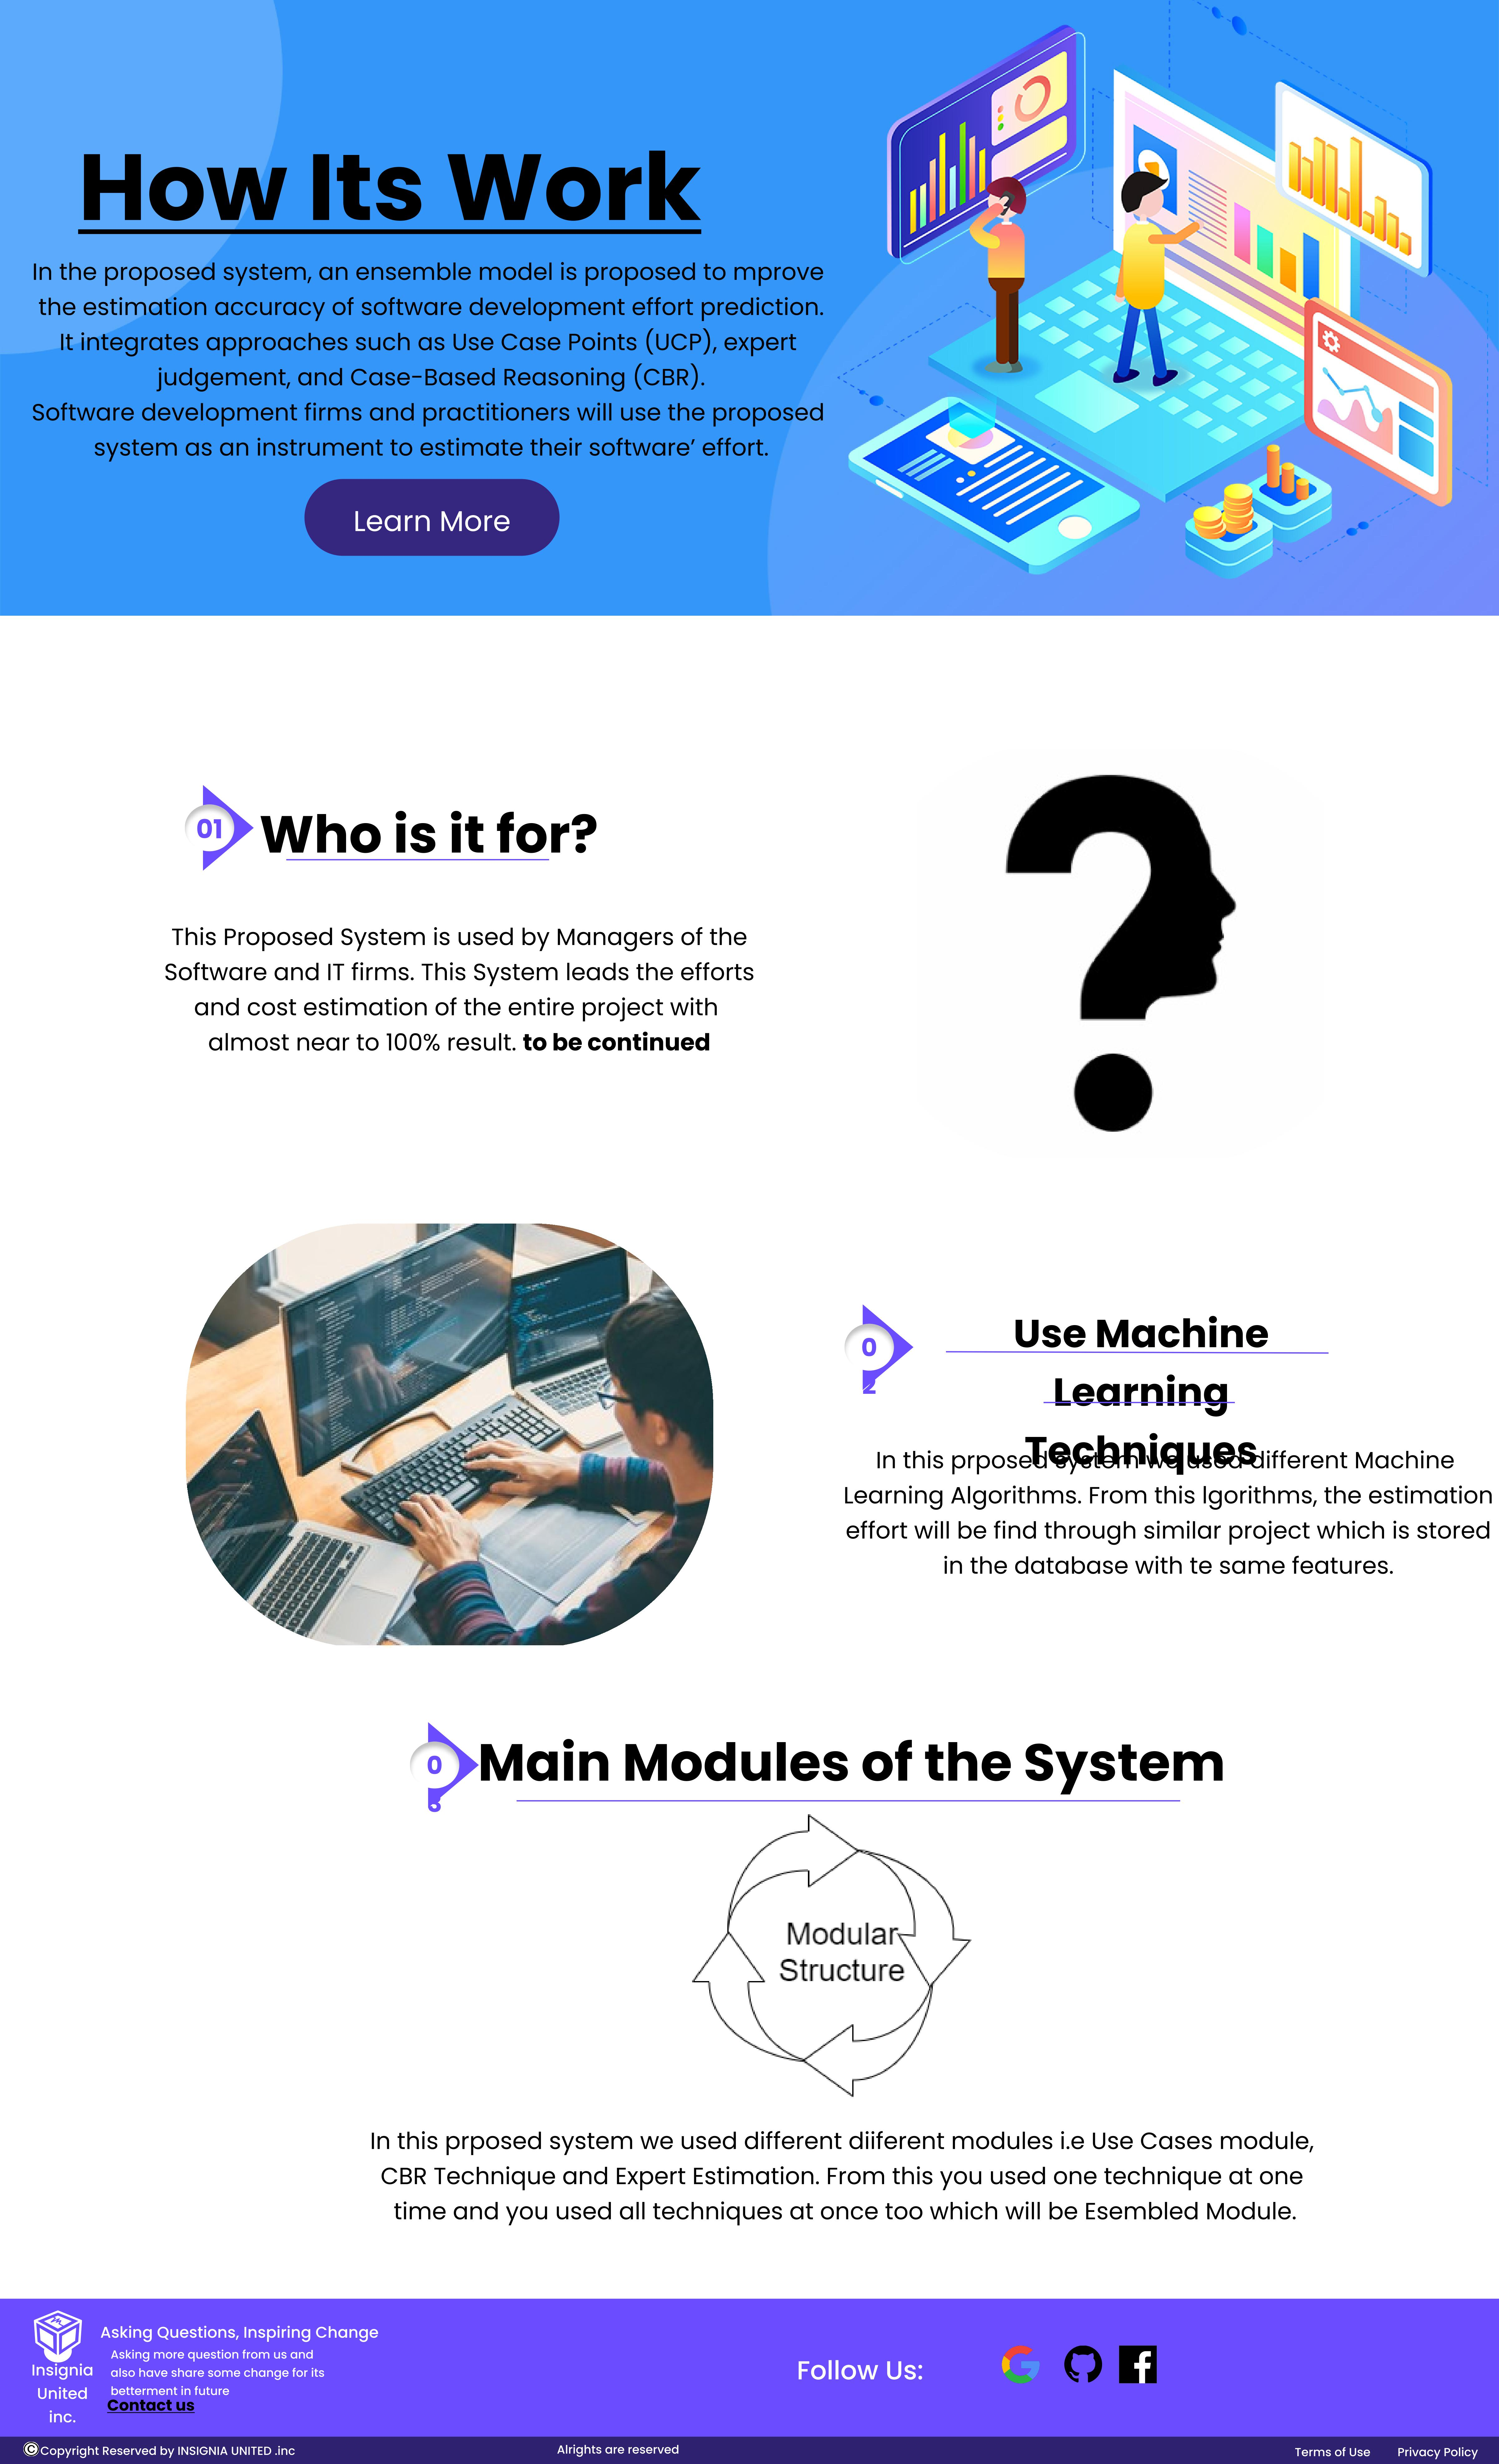
\includegraphics[height=10cm, width=0.9\textwidth]{./images/prototype/0009}
\centering 
\caption{Login Page}
\label{fig:prototype1}

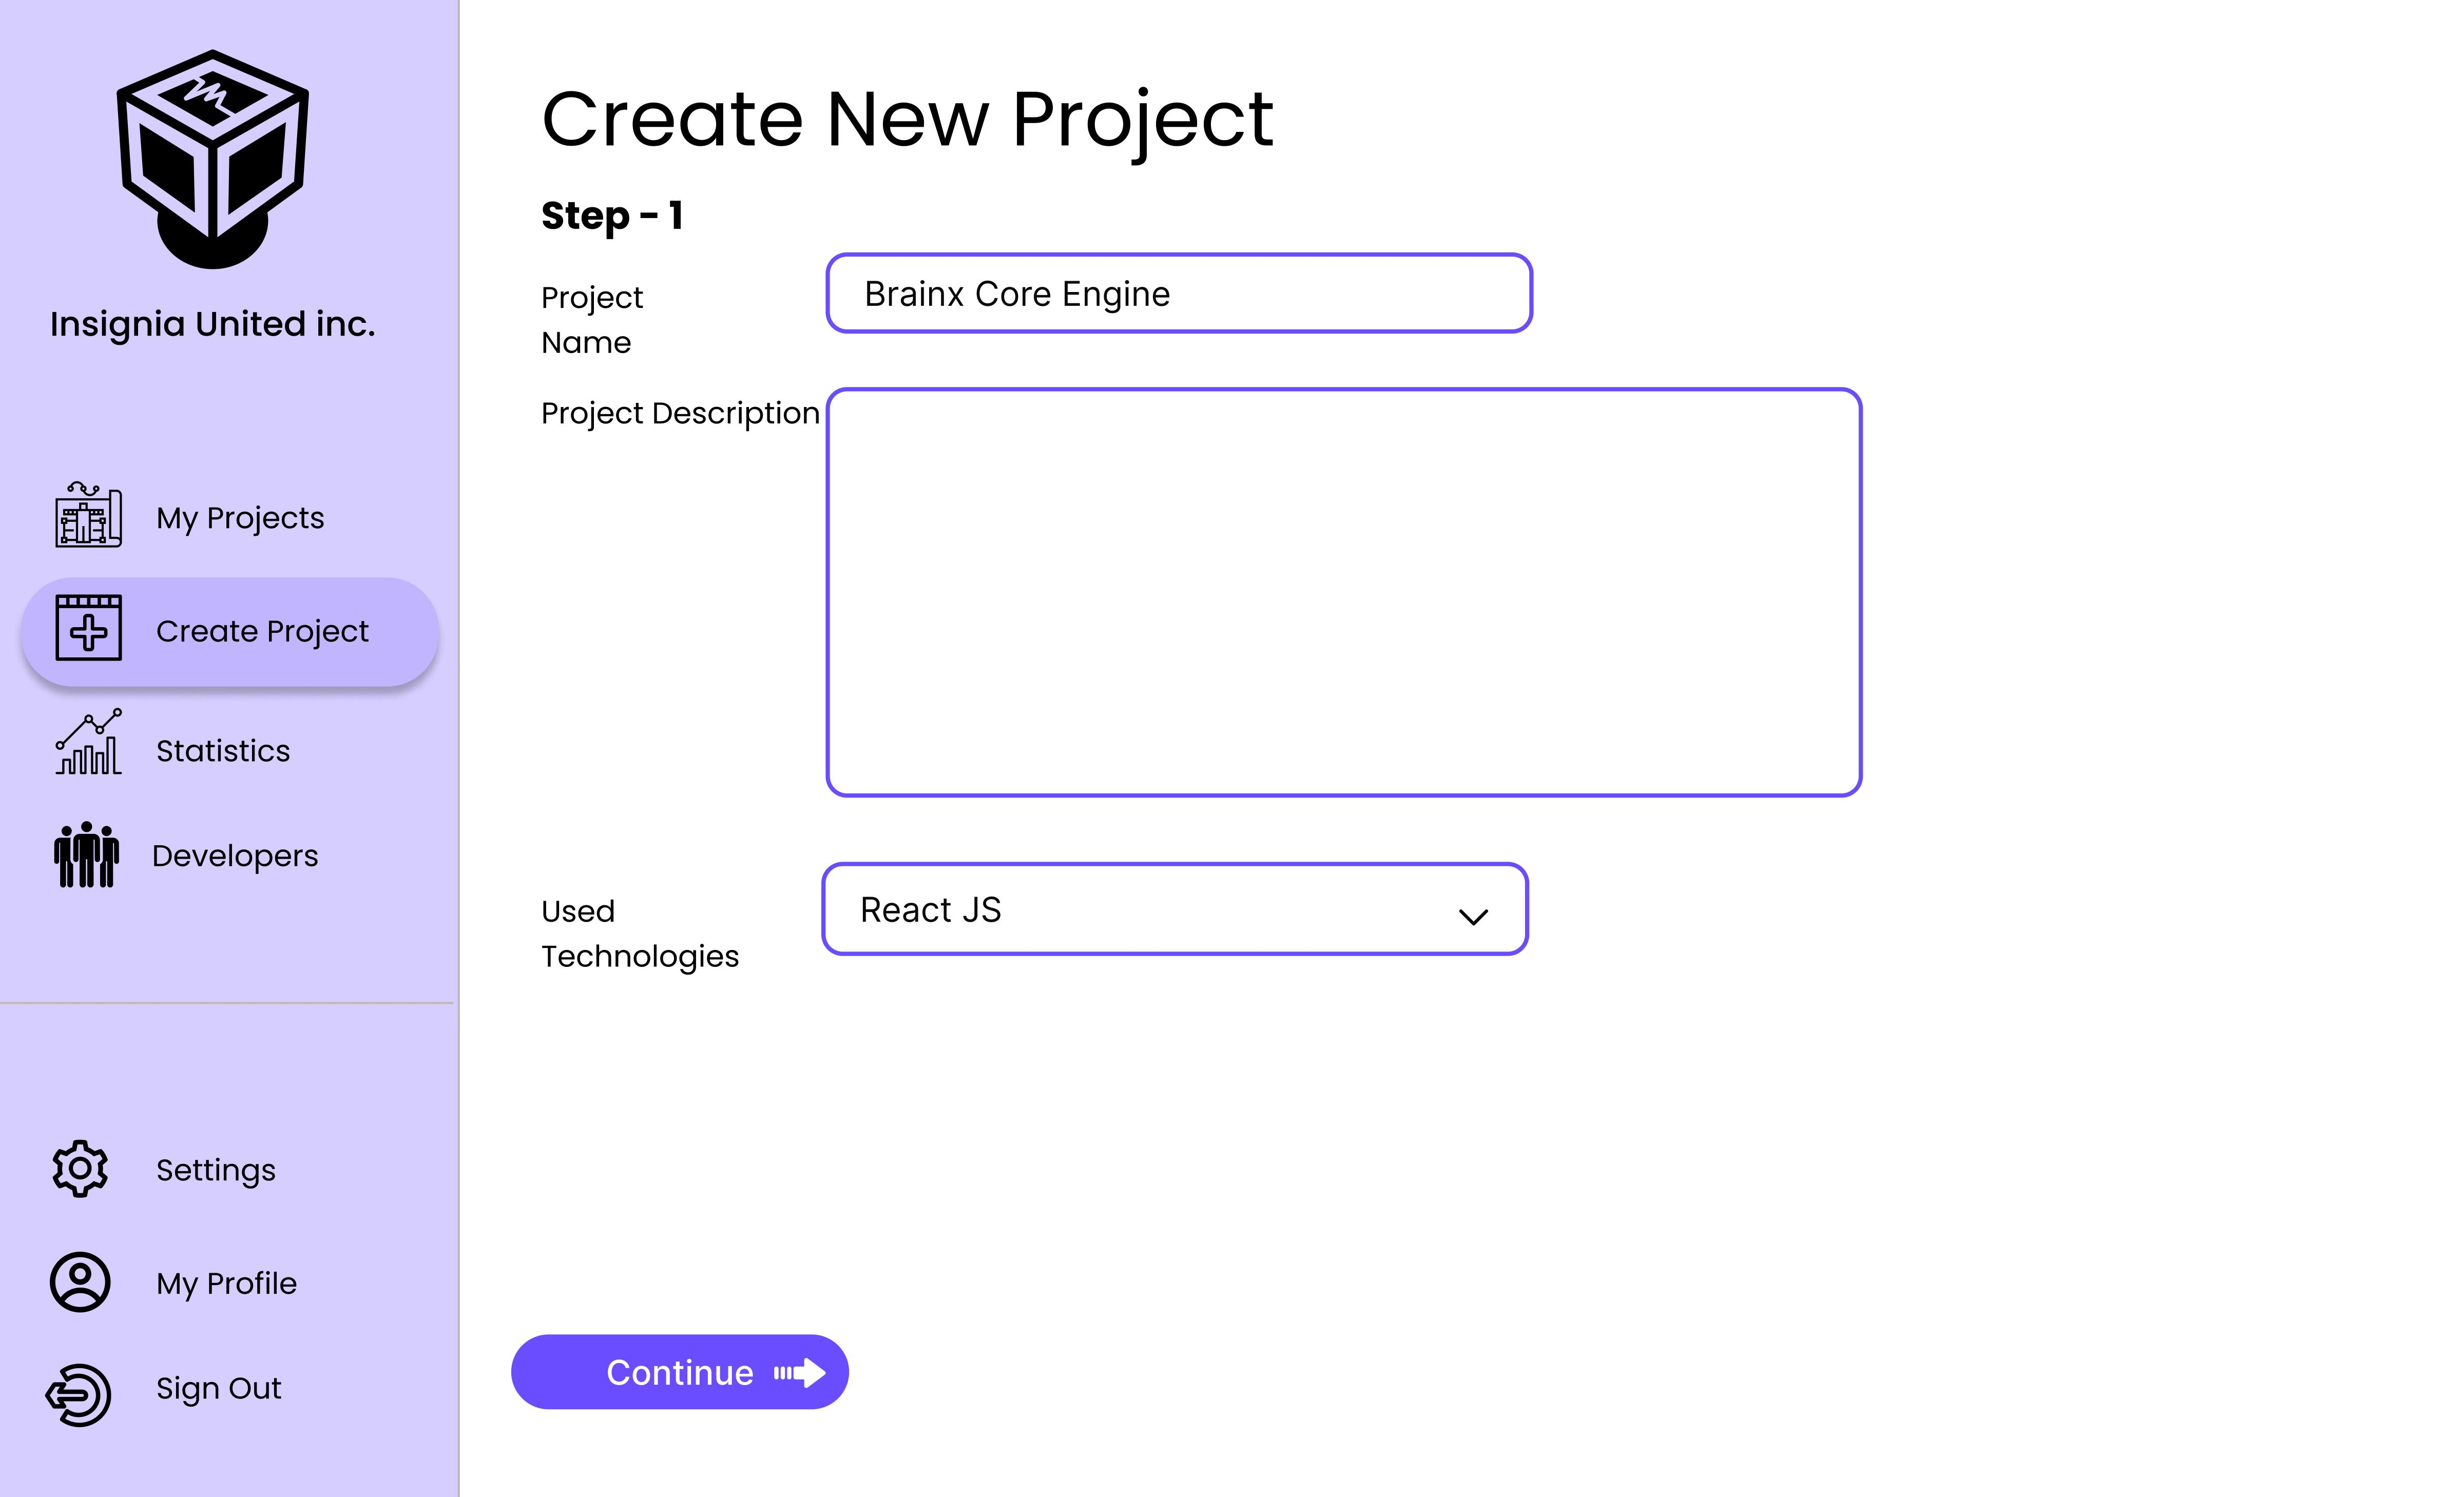
\includegraphics[height=10cm, width=0.9\textwidth]{./images/prototype/0010}
\centering 
\caption{Login Page}
\label{fig:prototype1}
\end{figure}

\begin{figure}[H]
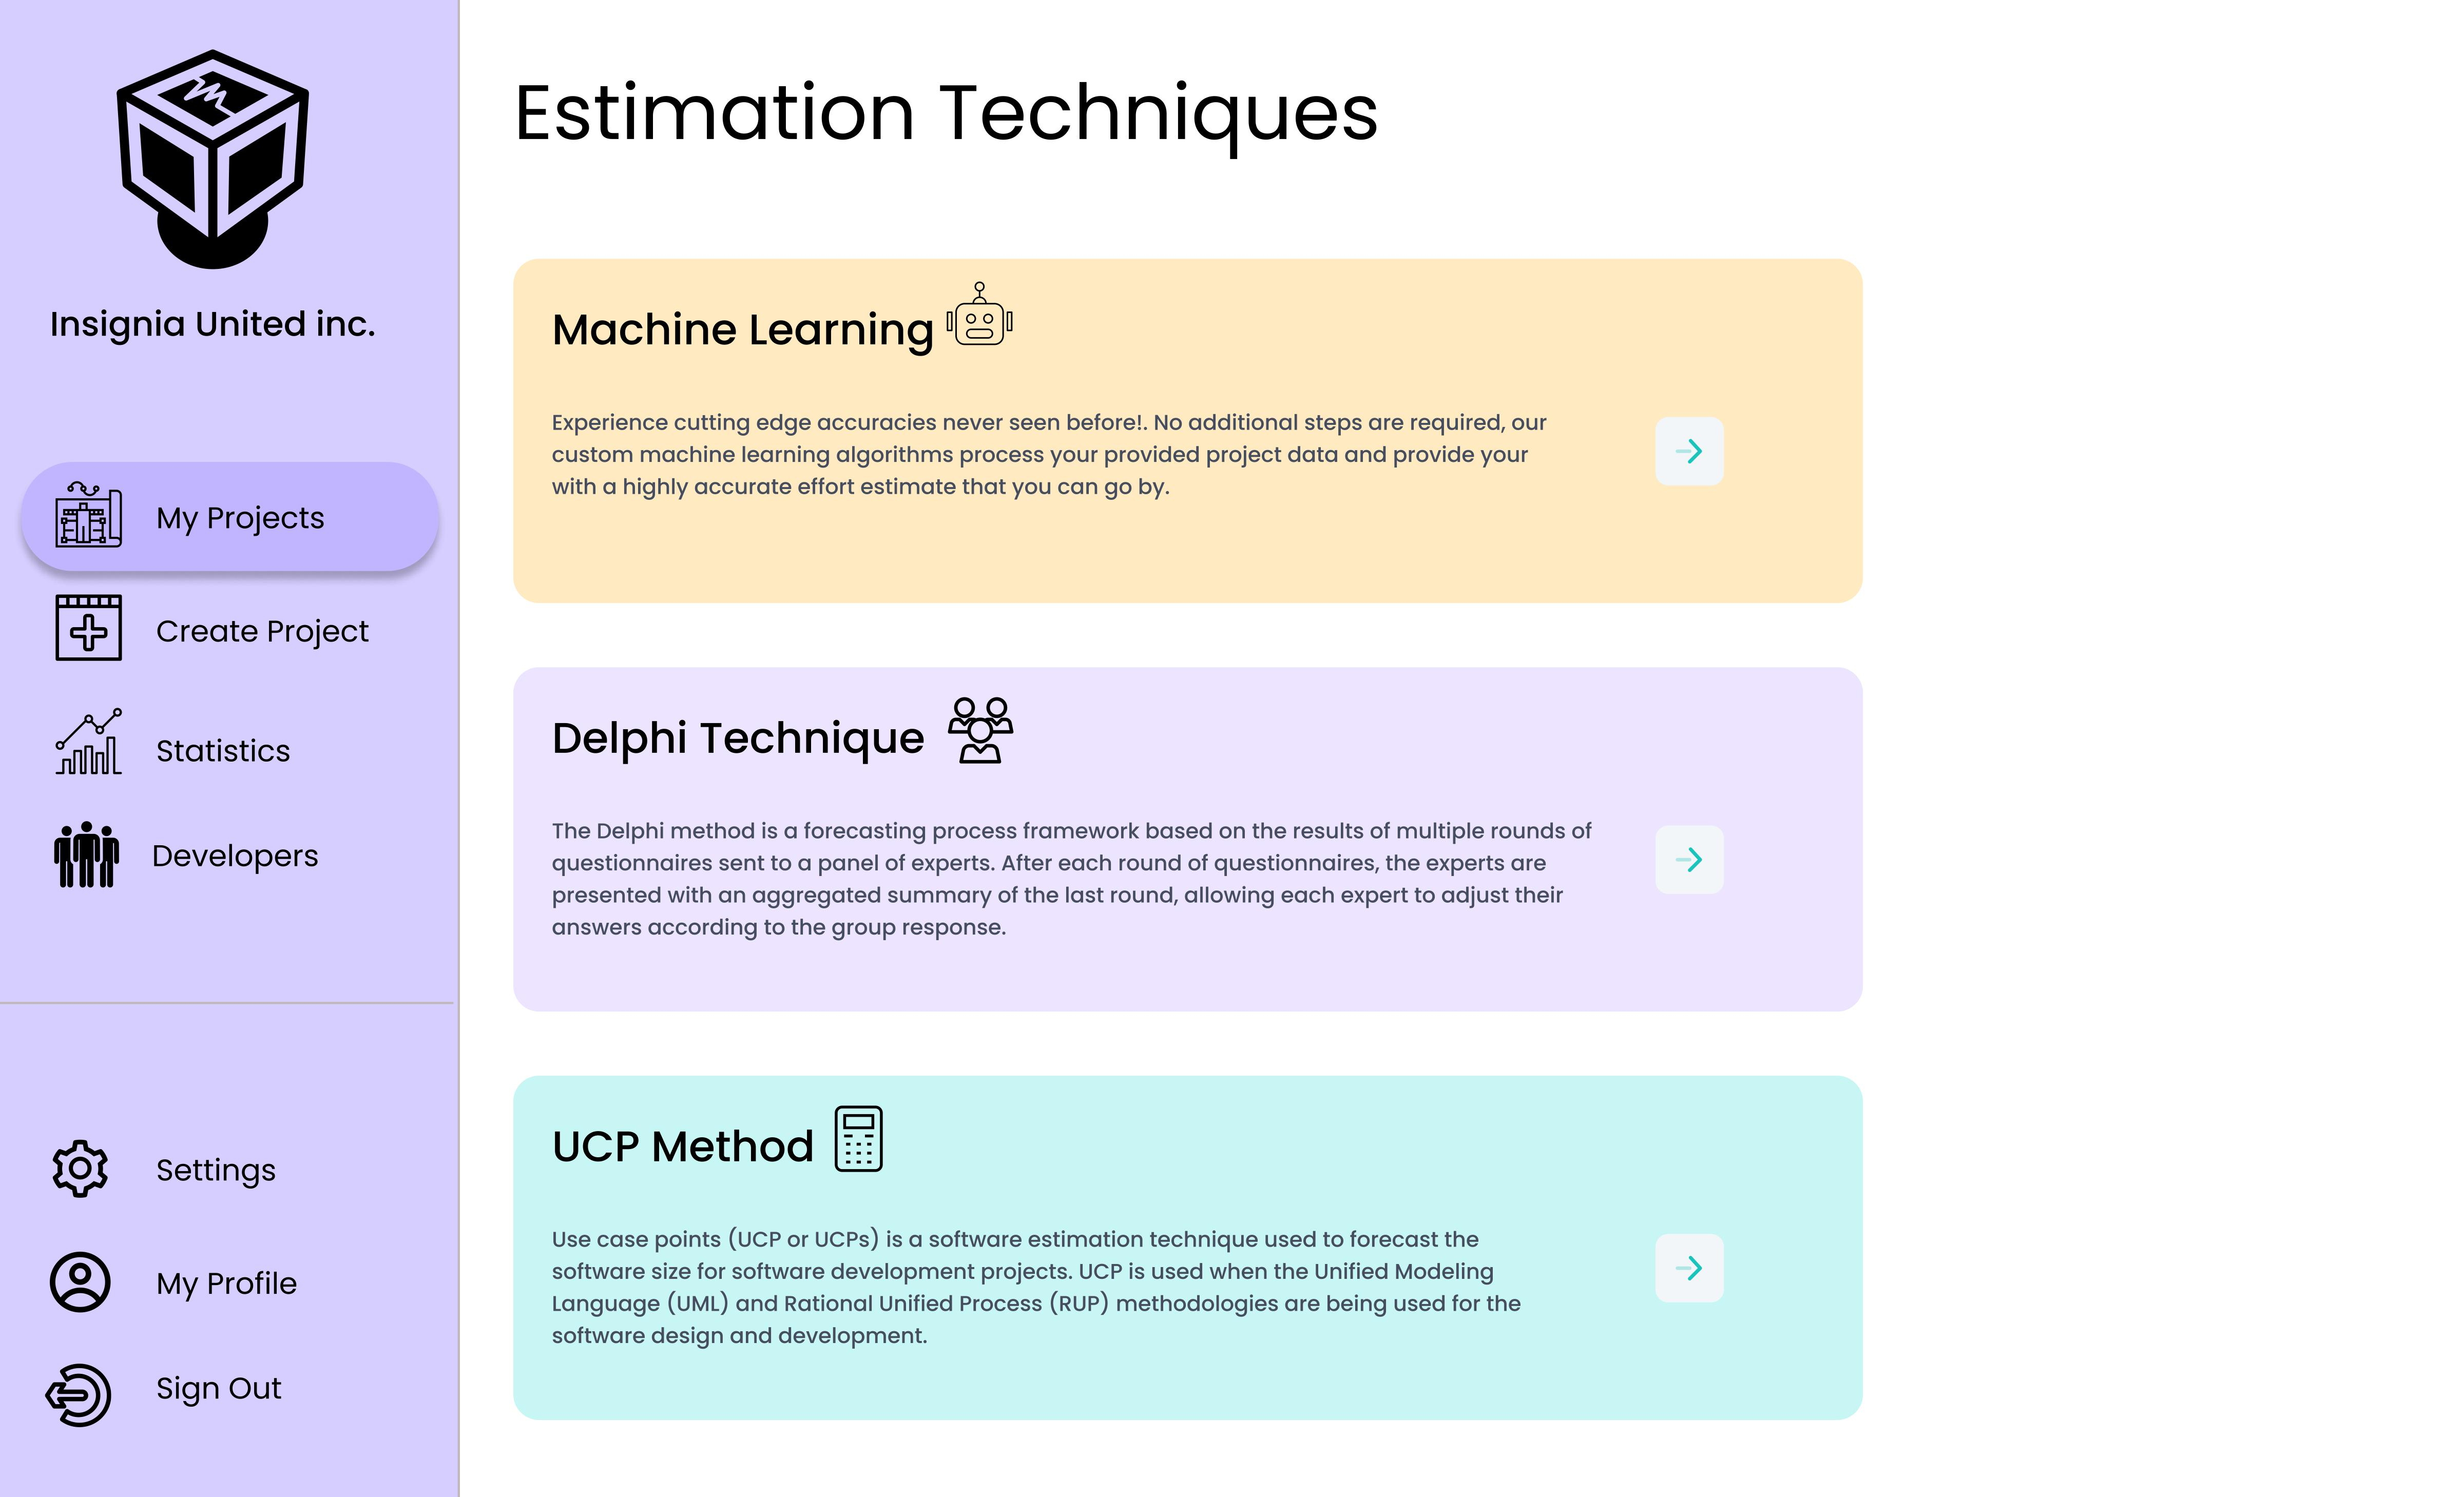
\includegraphics[height=10cm, width=0.9\textwidth]{./images/prototype/0011}
\centering 
\caption{Login Page}
\label{fig:prototype1}
\end{figure}

\begin{figure}[H]
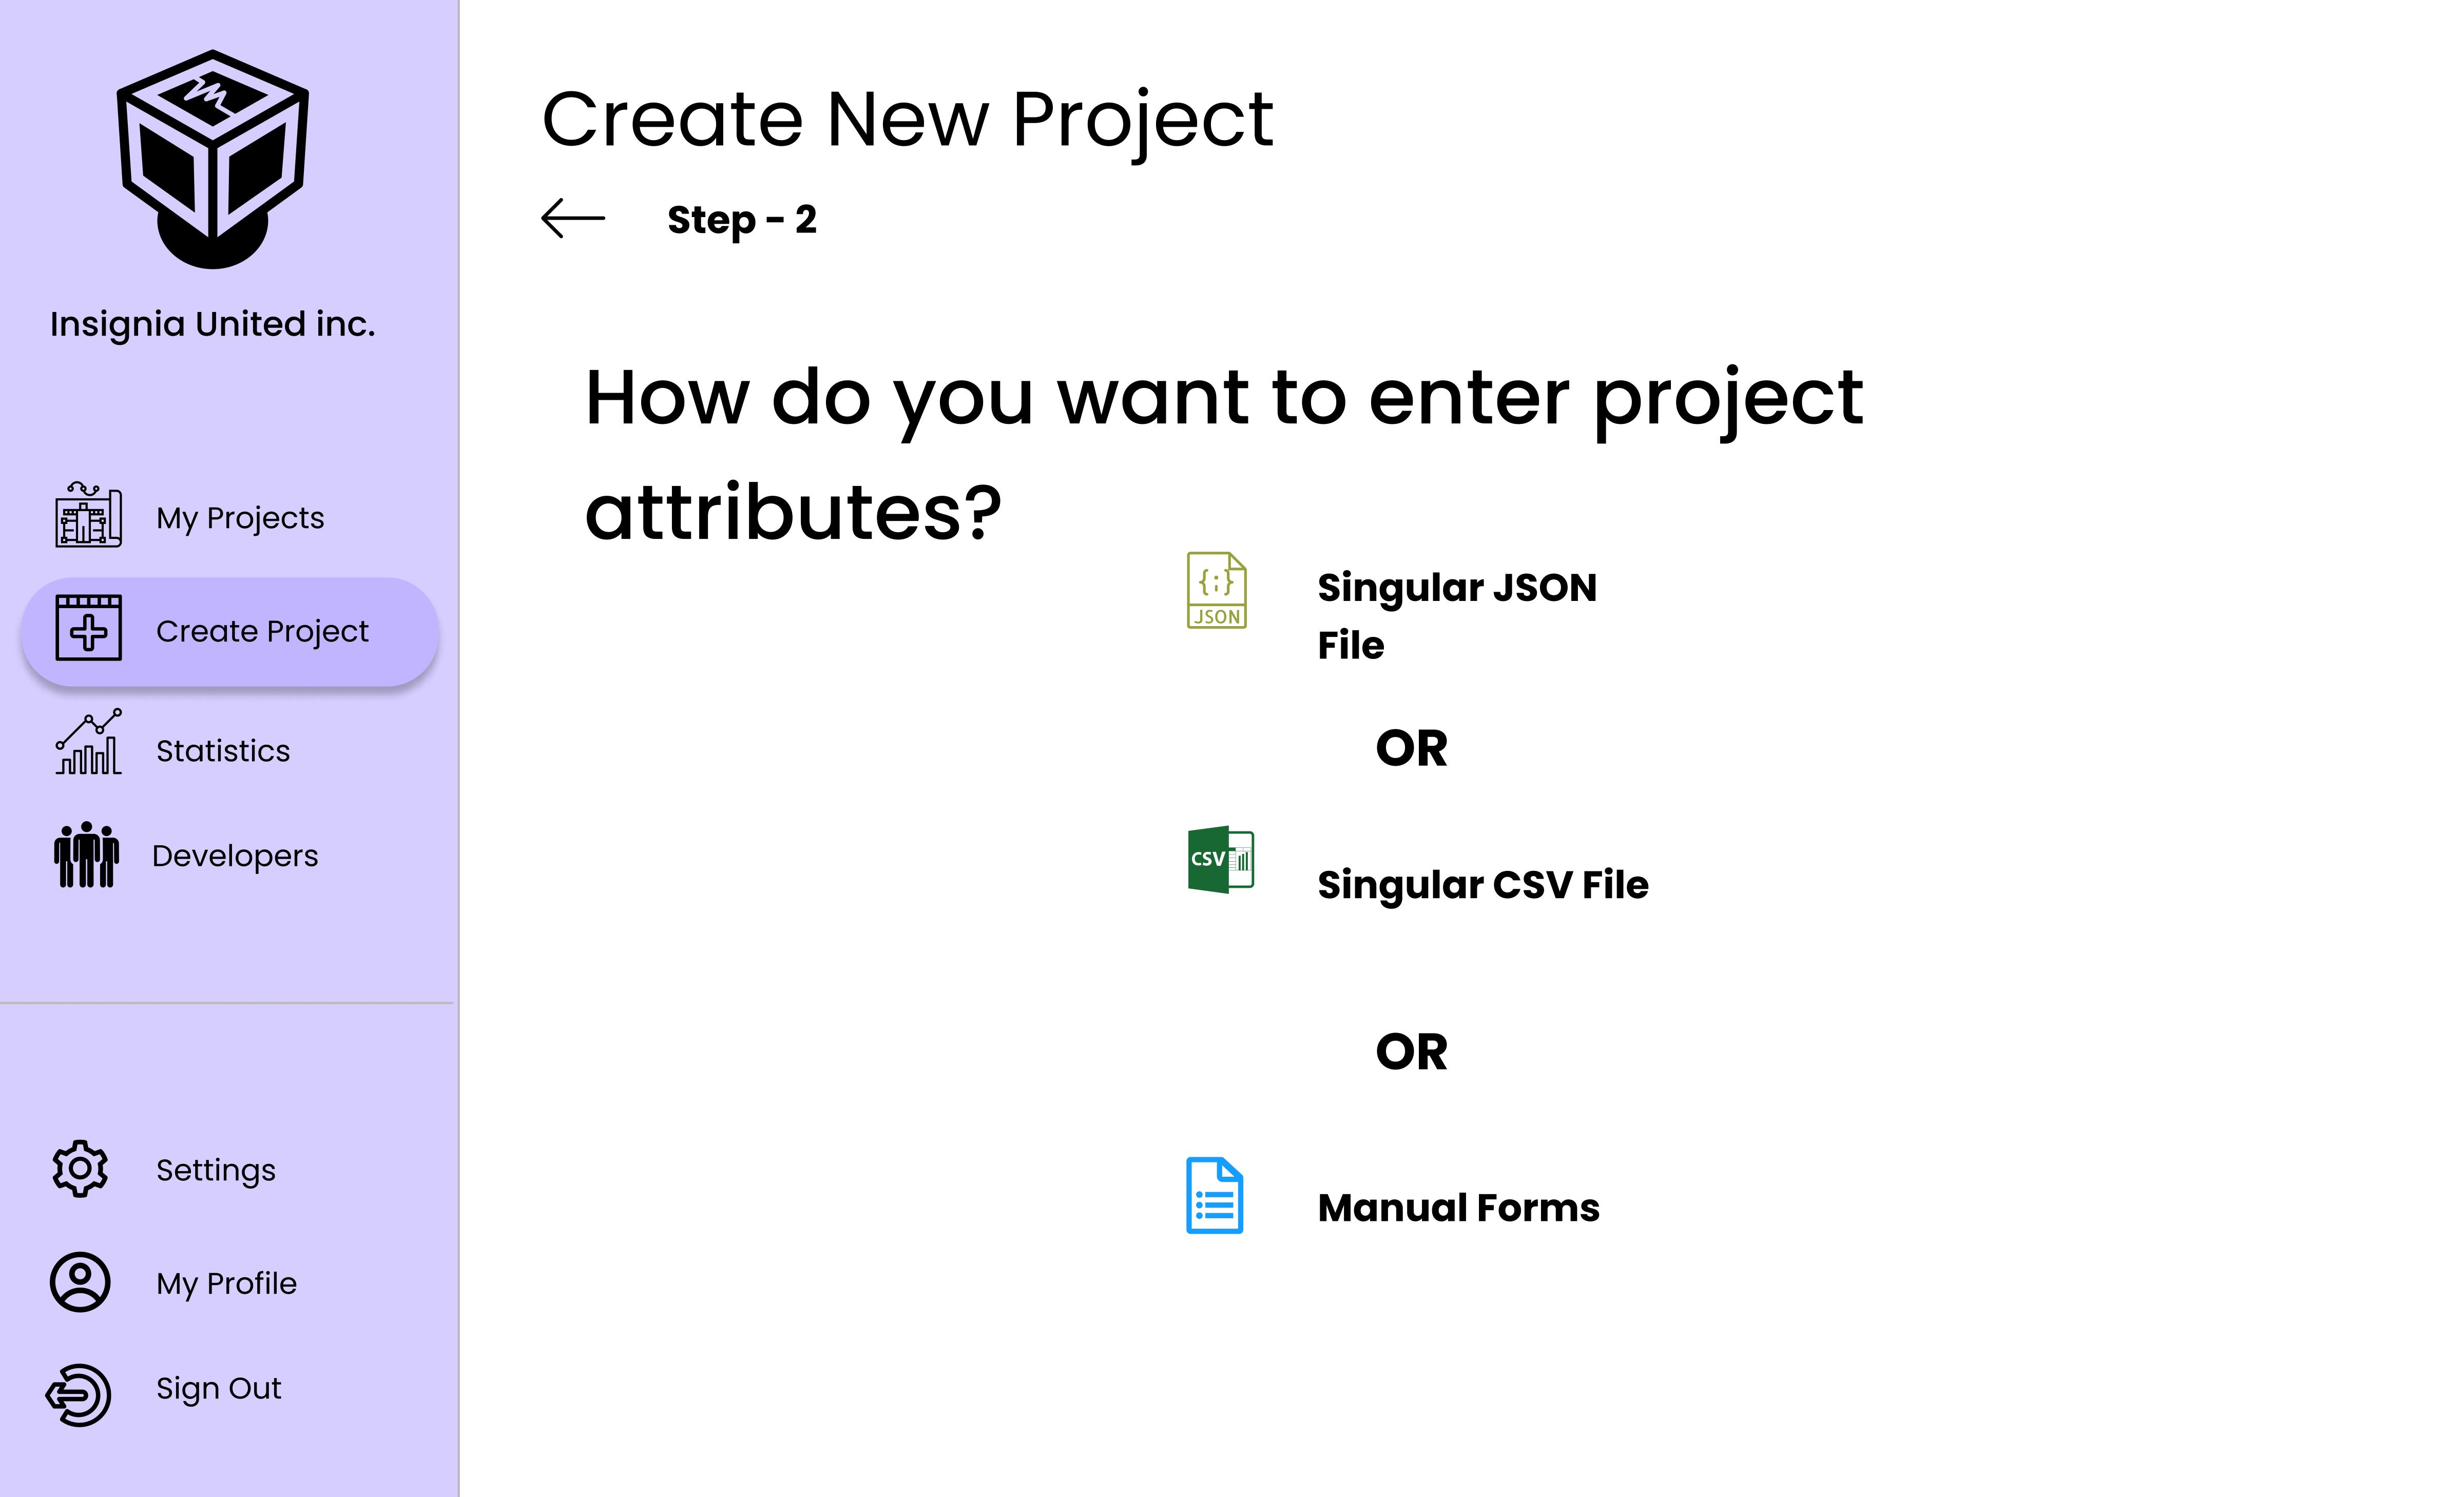
\includegraphics[height=10cm, width=0.9\textwidth]{./images/prototype/0012}
\centering 
\caption{Login Page}
\label{fig:prototype1}

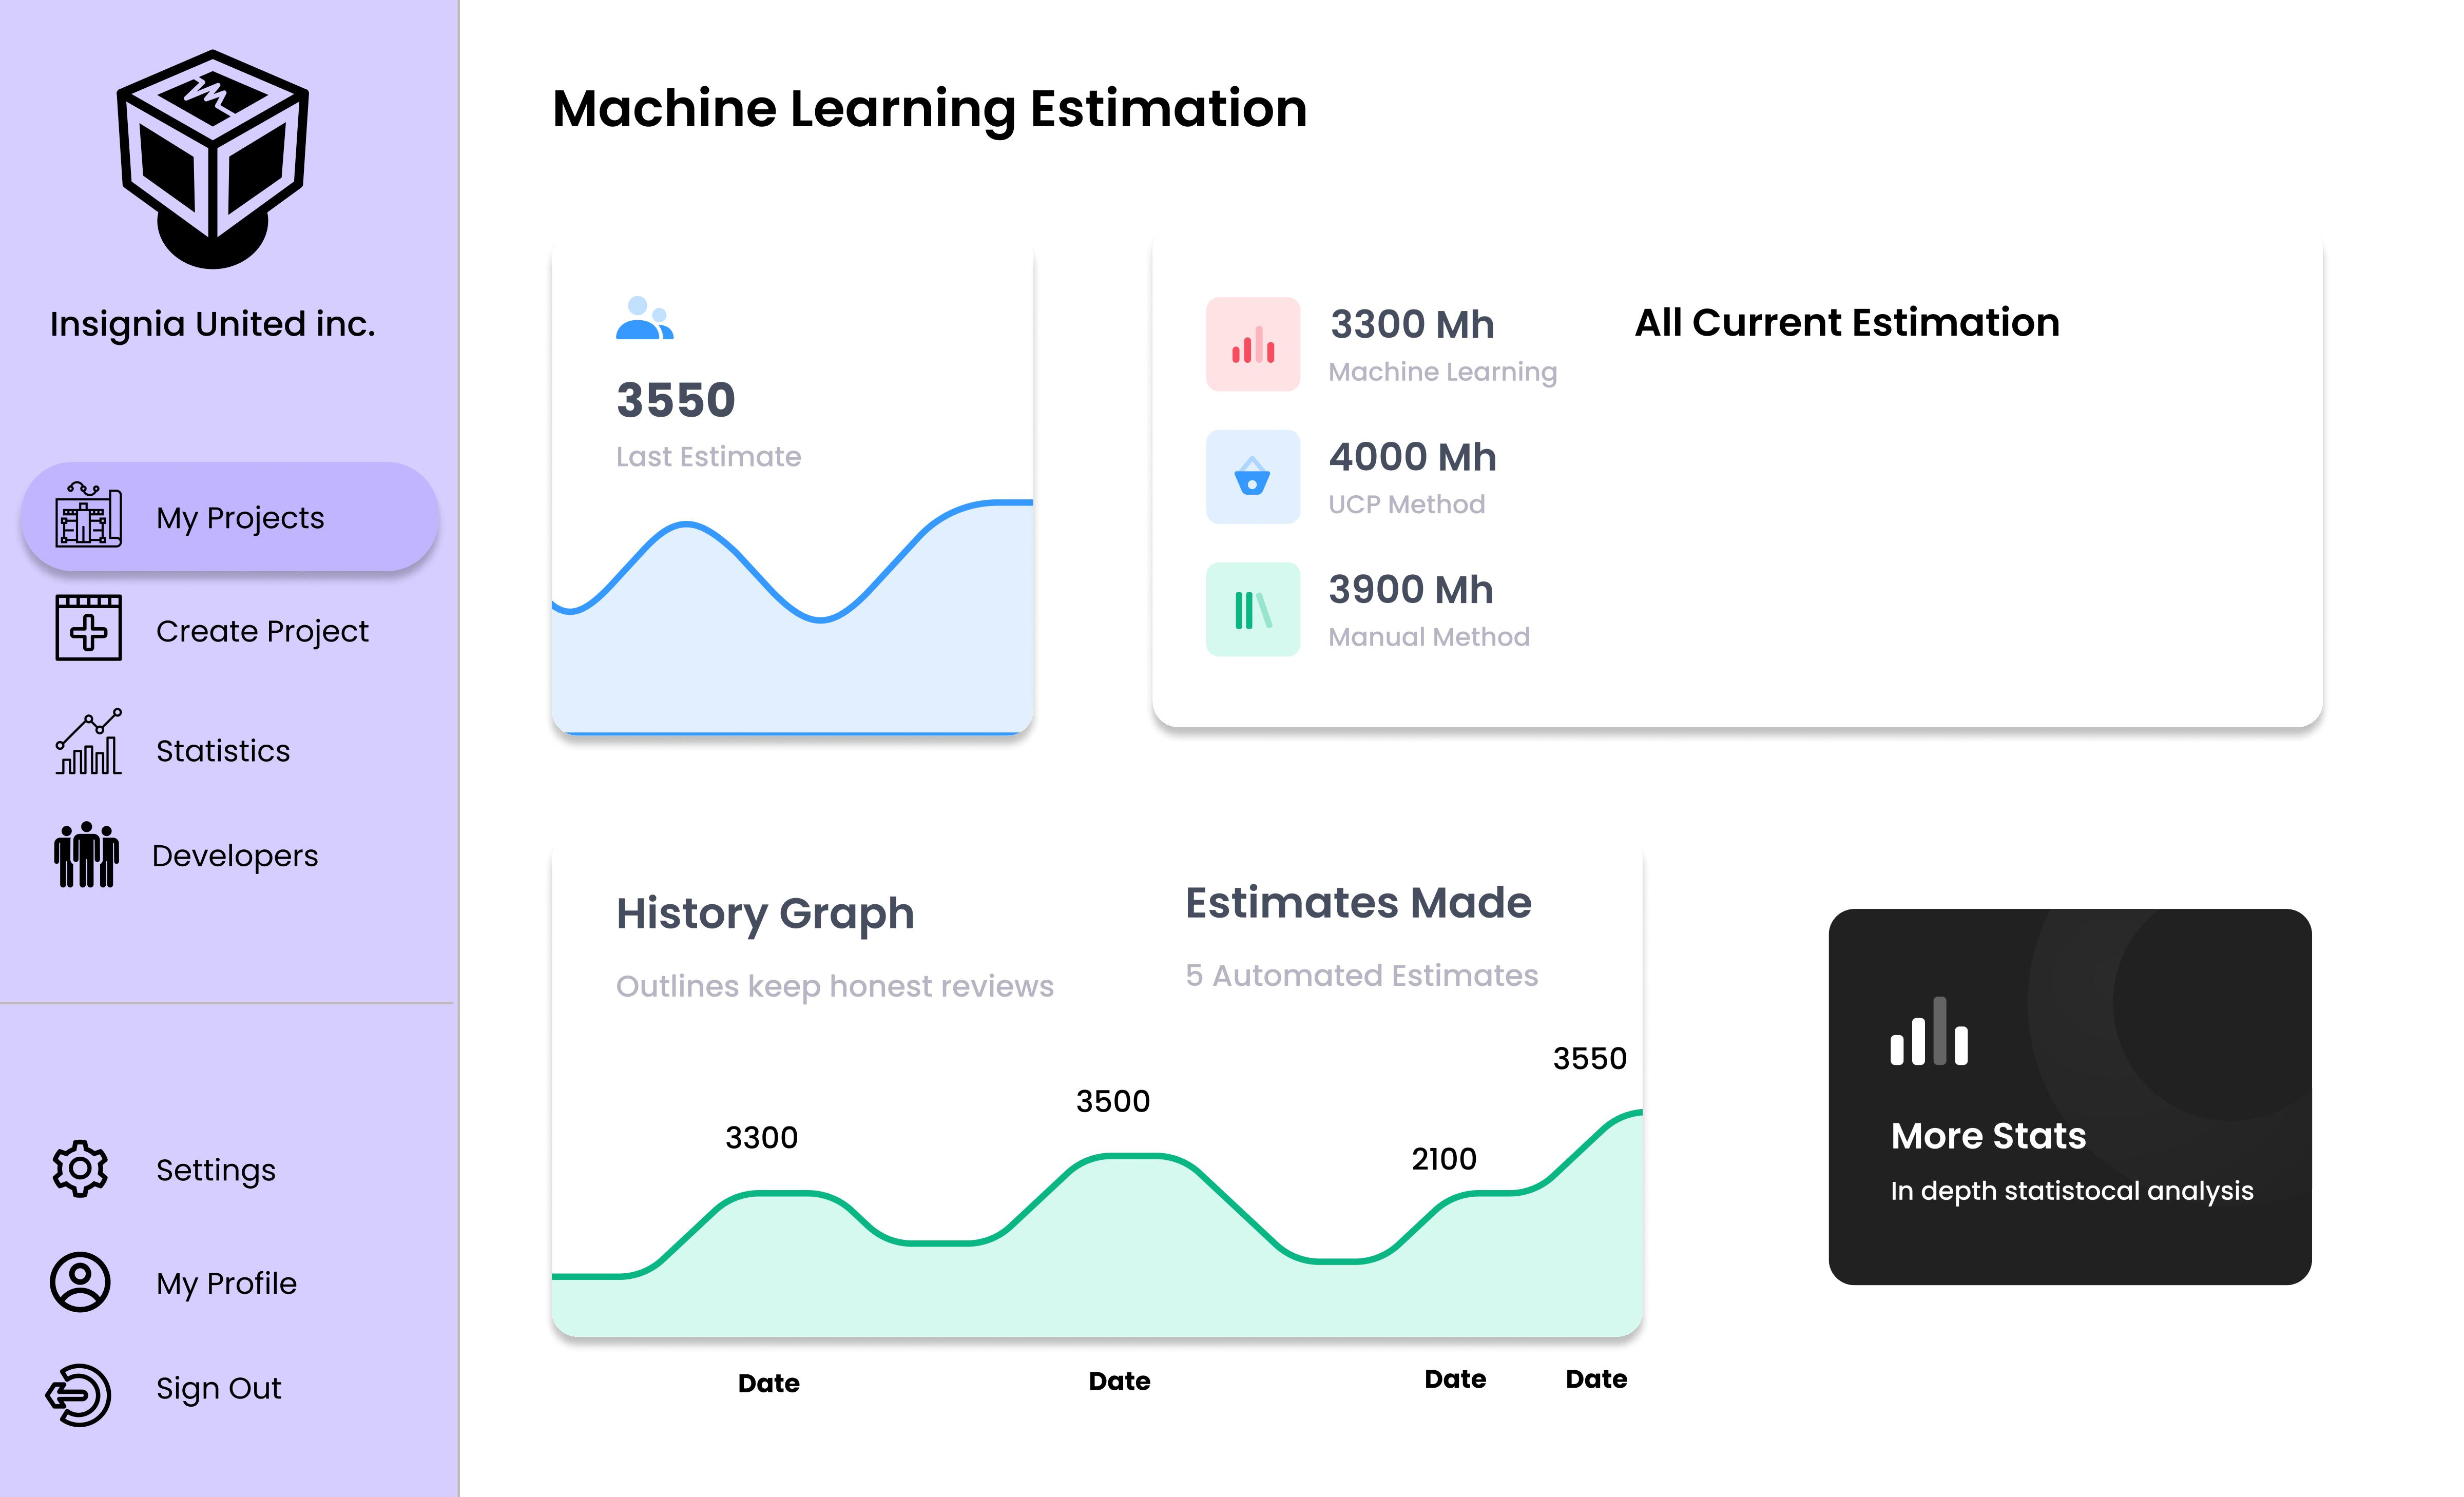
\includegraphics[height=10cm, width=0.9\textwidth]{./images/prototype/0013}
\centering 
\caption{Login Page}
\label{fig:prototype1}
\end{figure}

\begin{figure}[H]
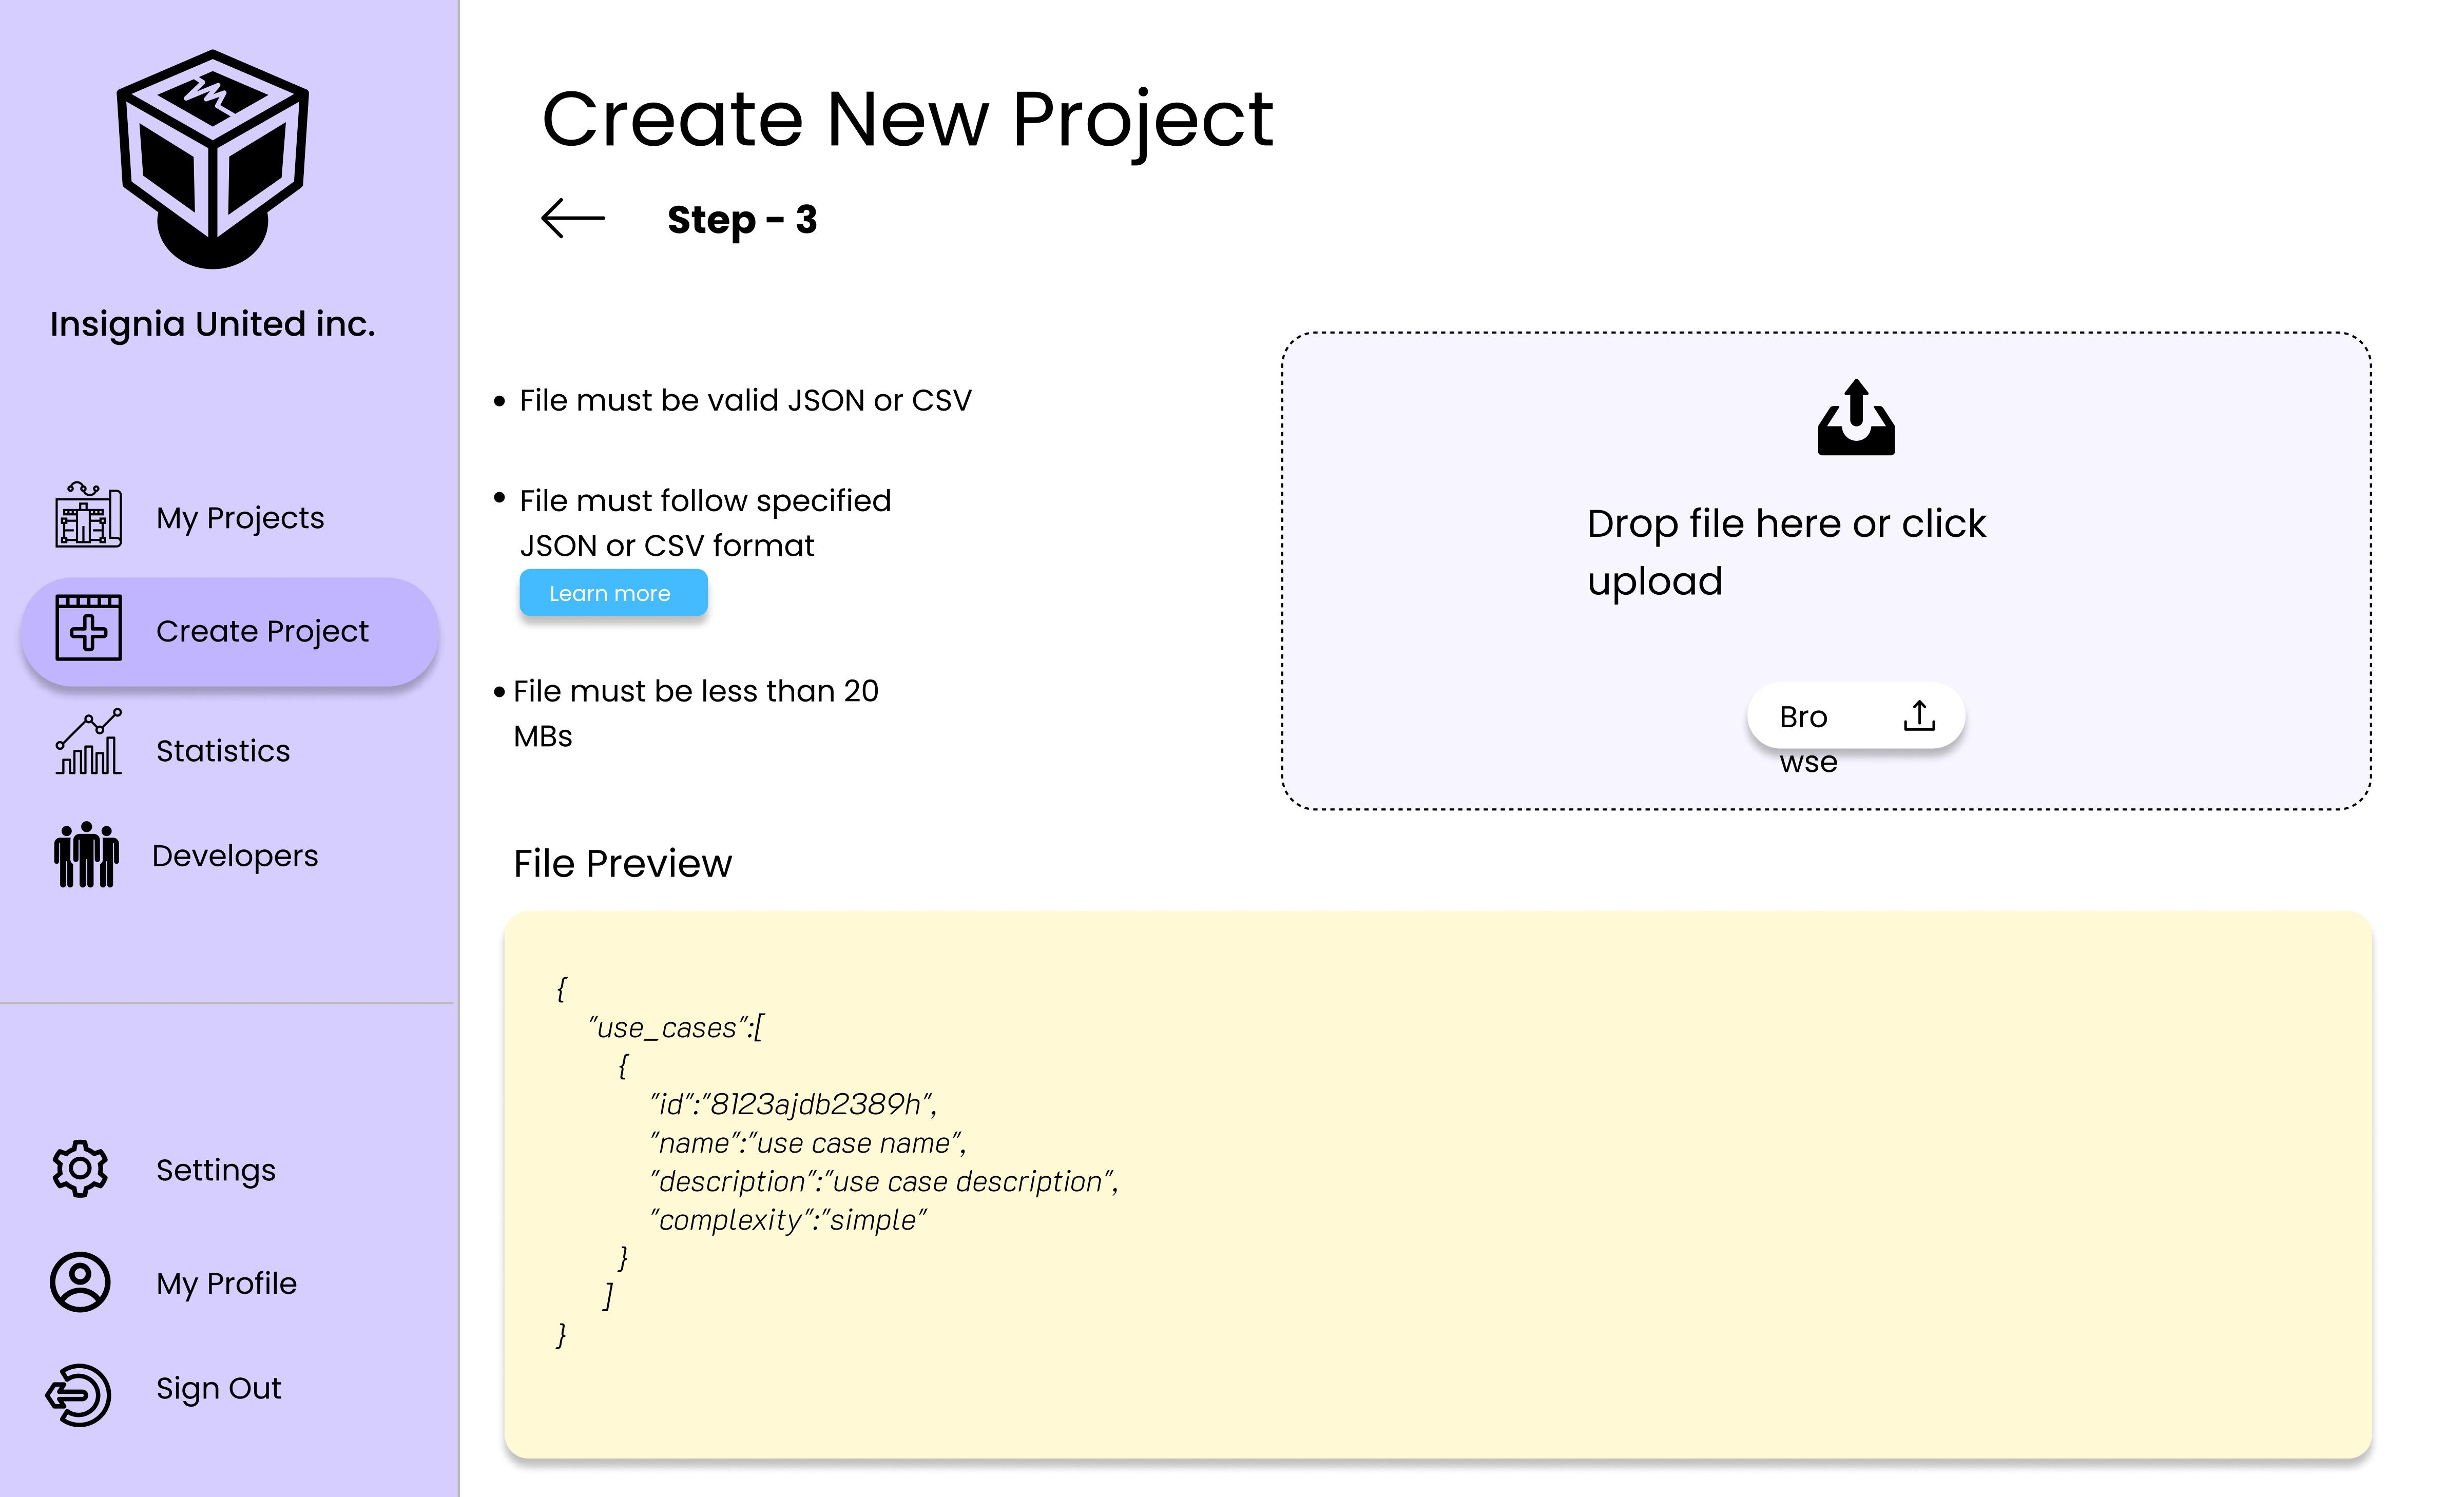
\includegraphics[height=10cm, width=0.9\textwidth]{./images/prototype/0014}
\centering 
\caption{Login Page}
\label{fig:prototype1}

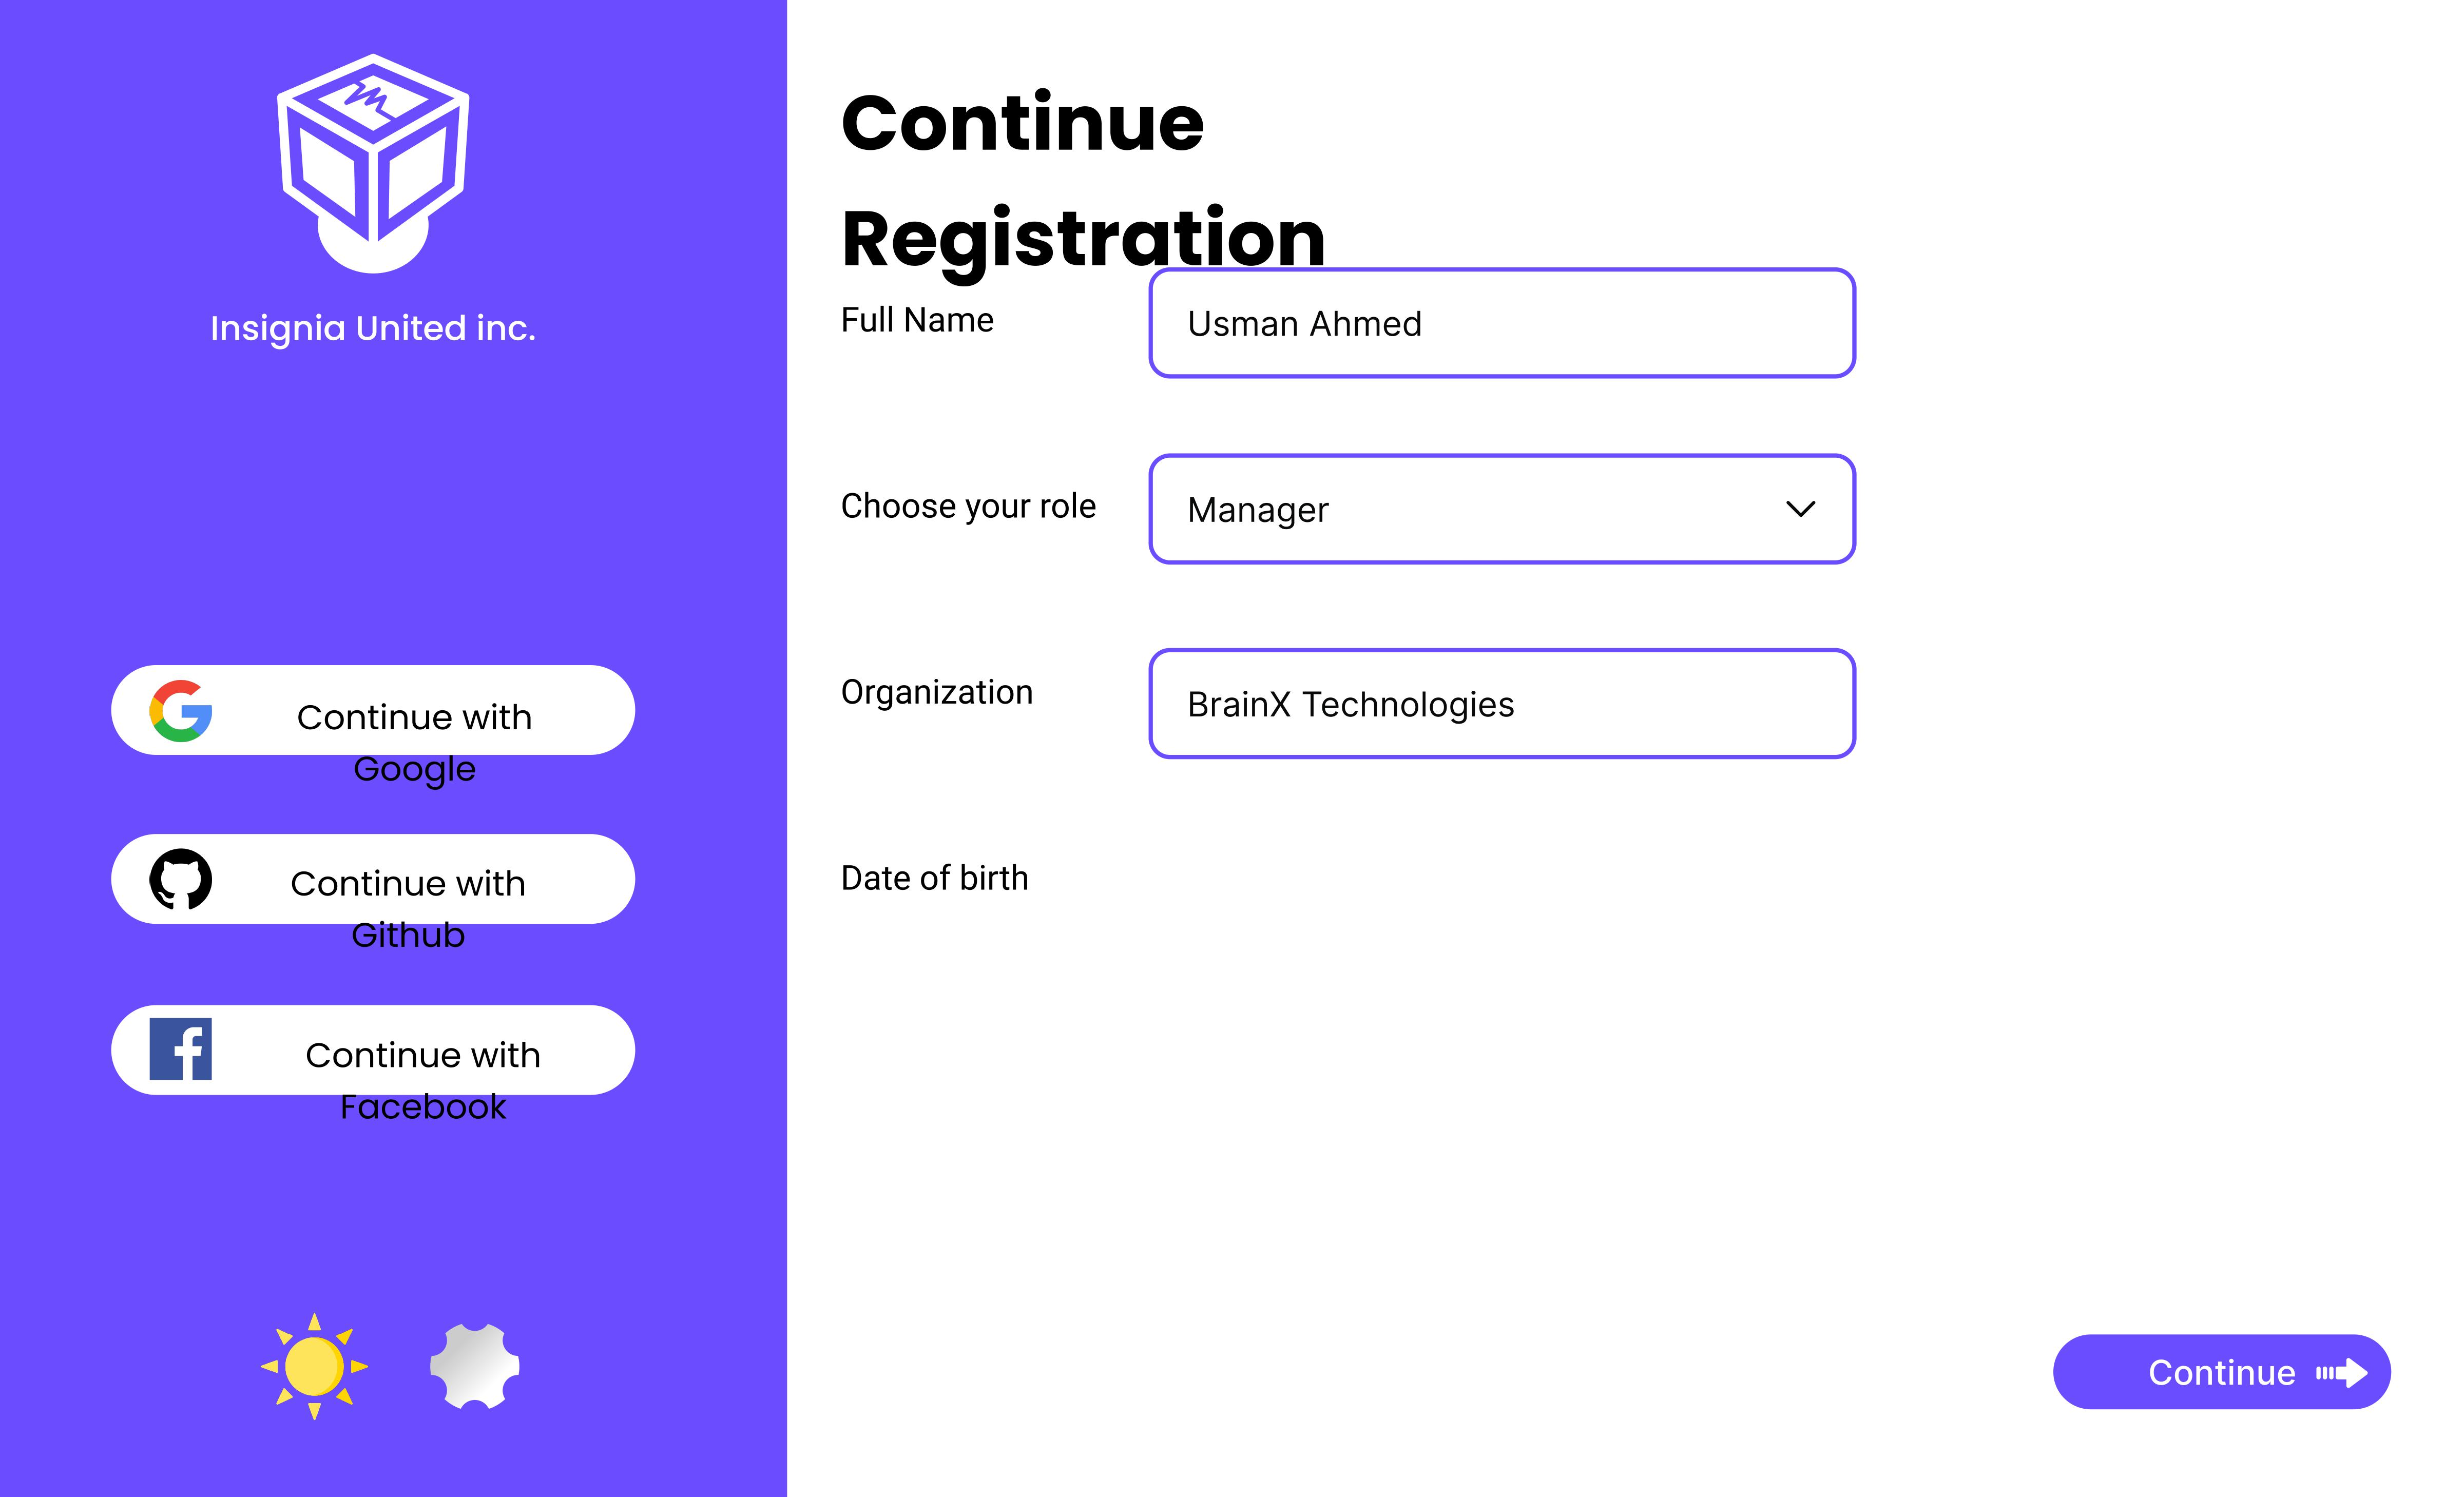
\includegraphics[height=10cm, width=0.9\textwidth]{./images/prototype/0015}
\centering 
\caption{Login Page}
\label{fig:prototype1}
\end{figure}

\begin{figure}[H]
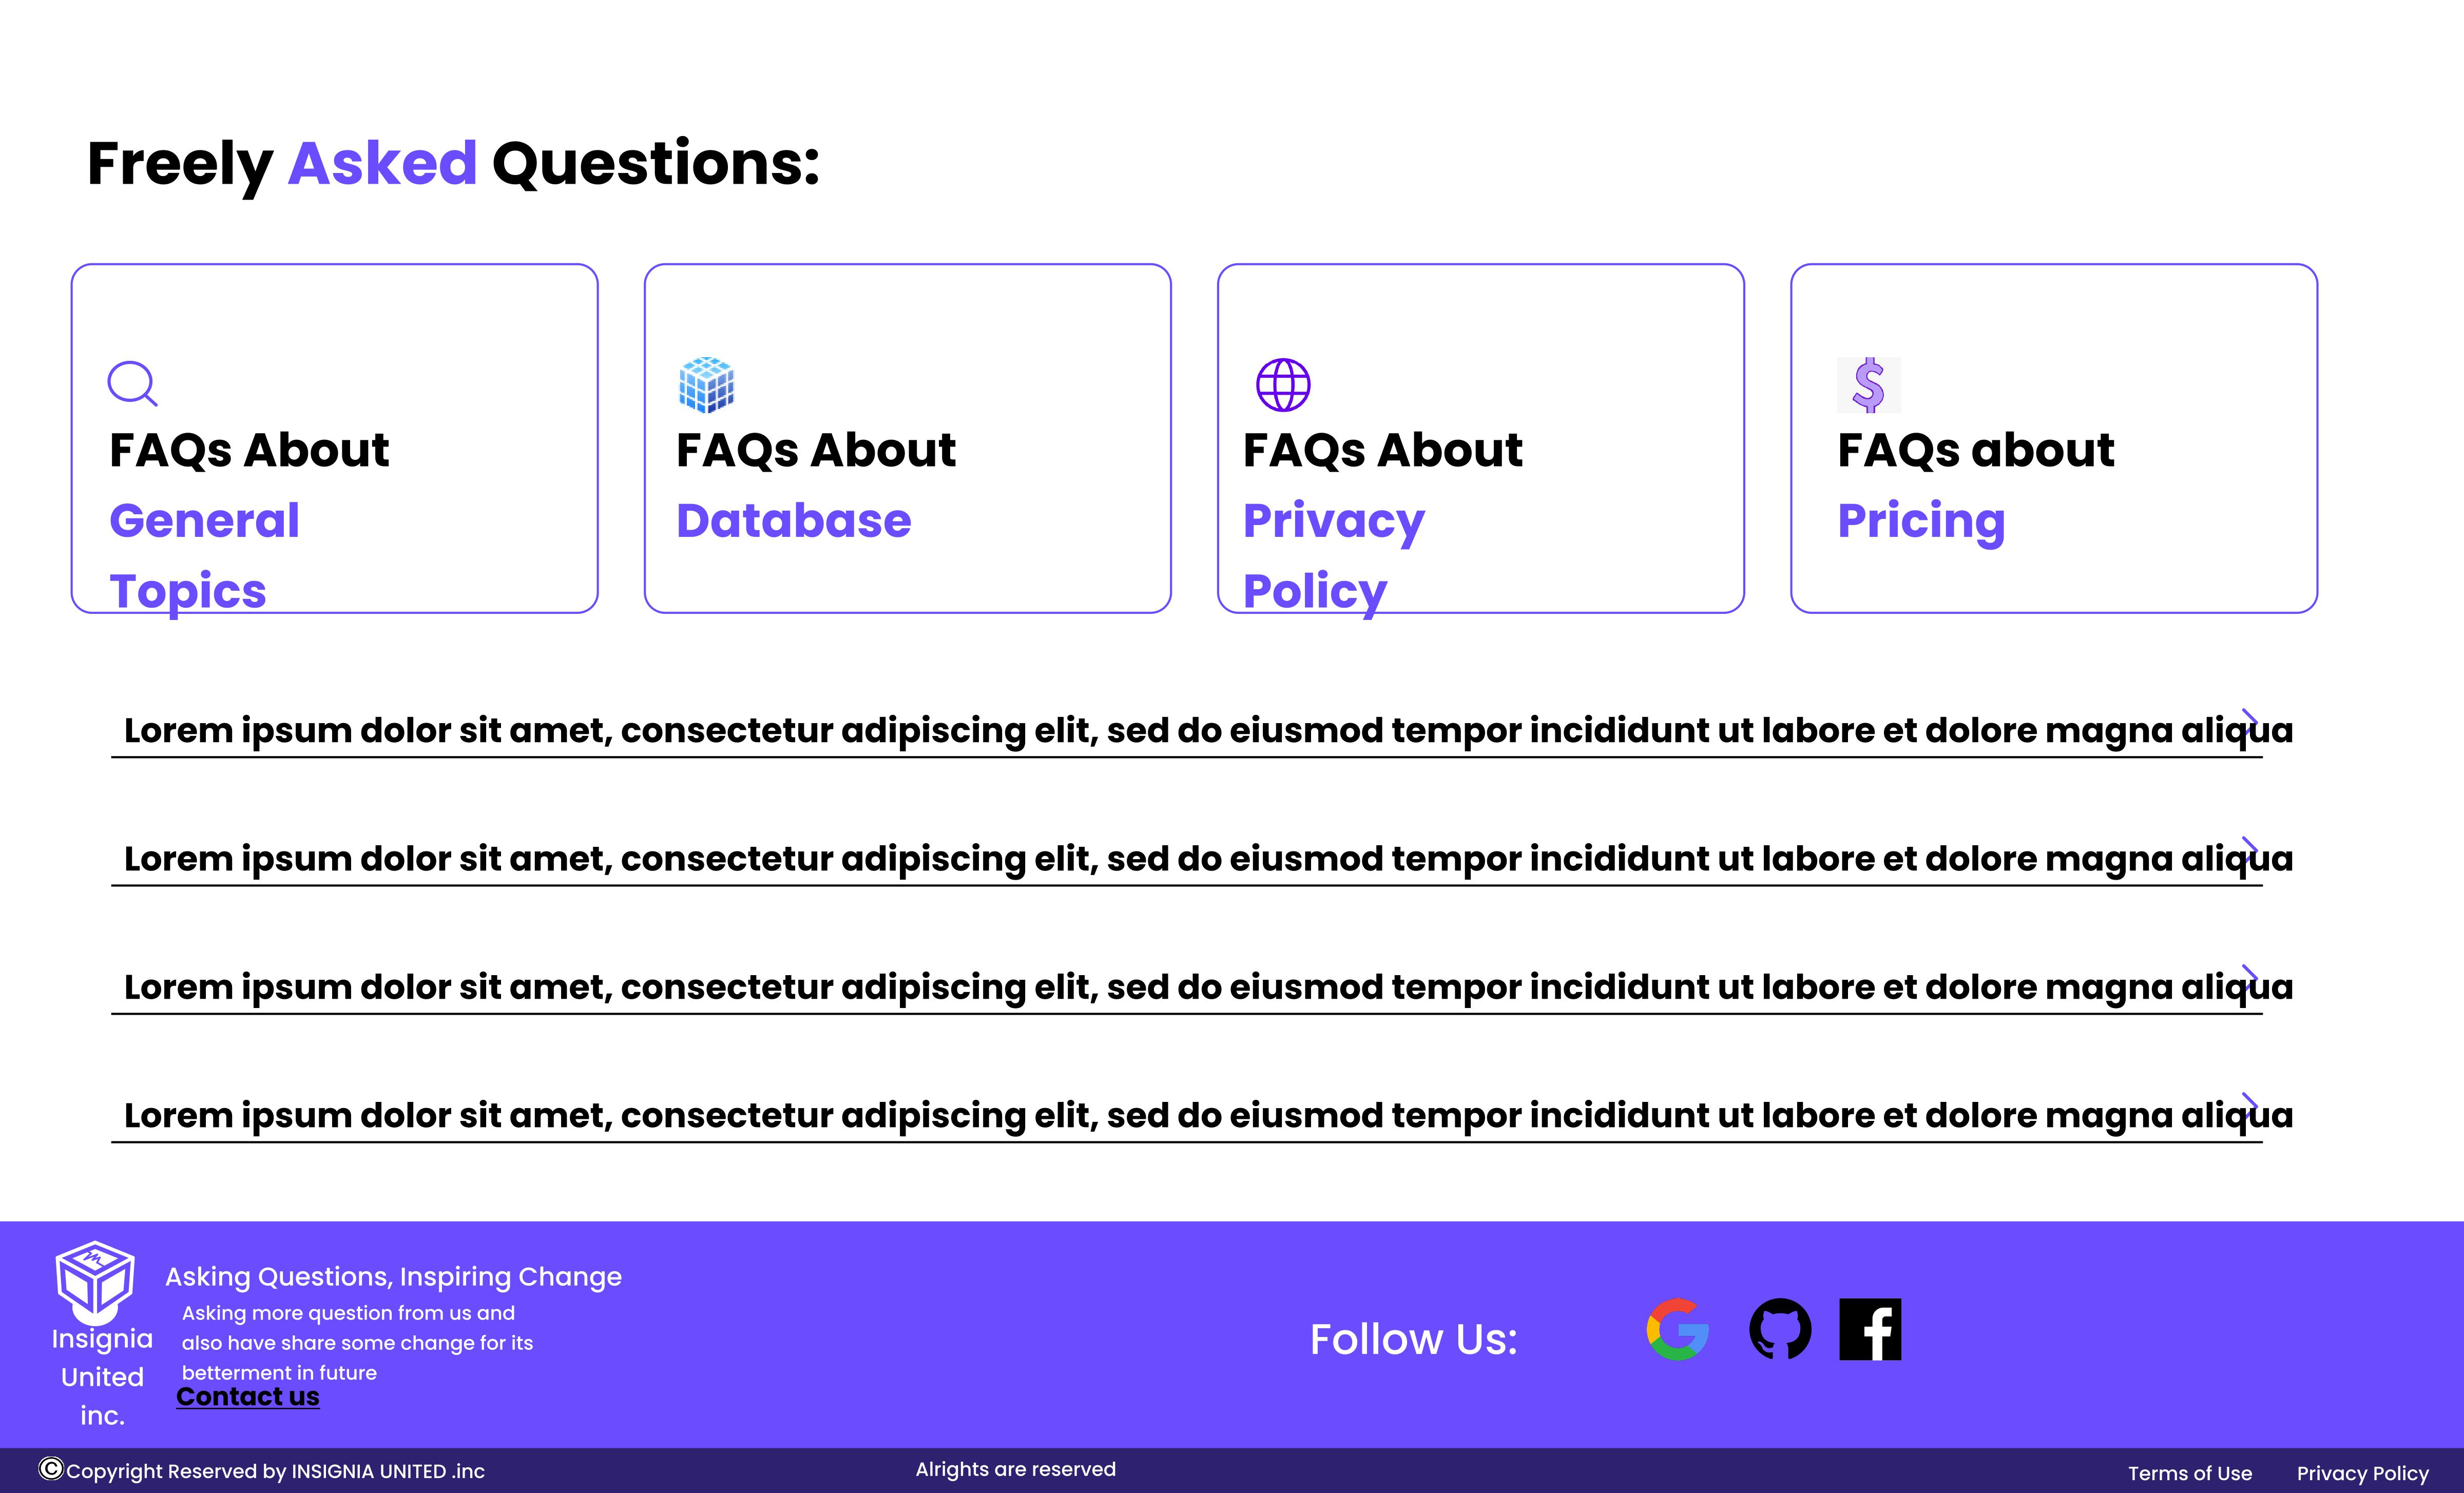
\includegraphics[height=10cm, width=0.9\textwidth]{./images/prototype/0016}
\centering 
\caption{Login Page}
\label{fig:prototype1}

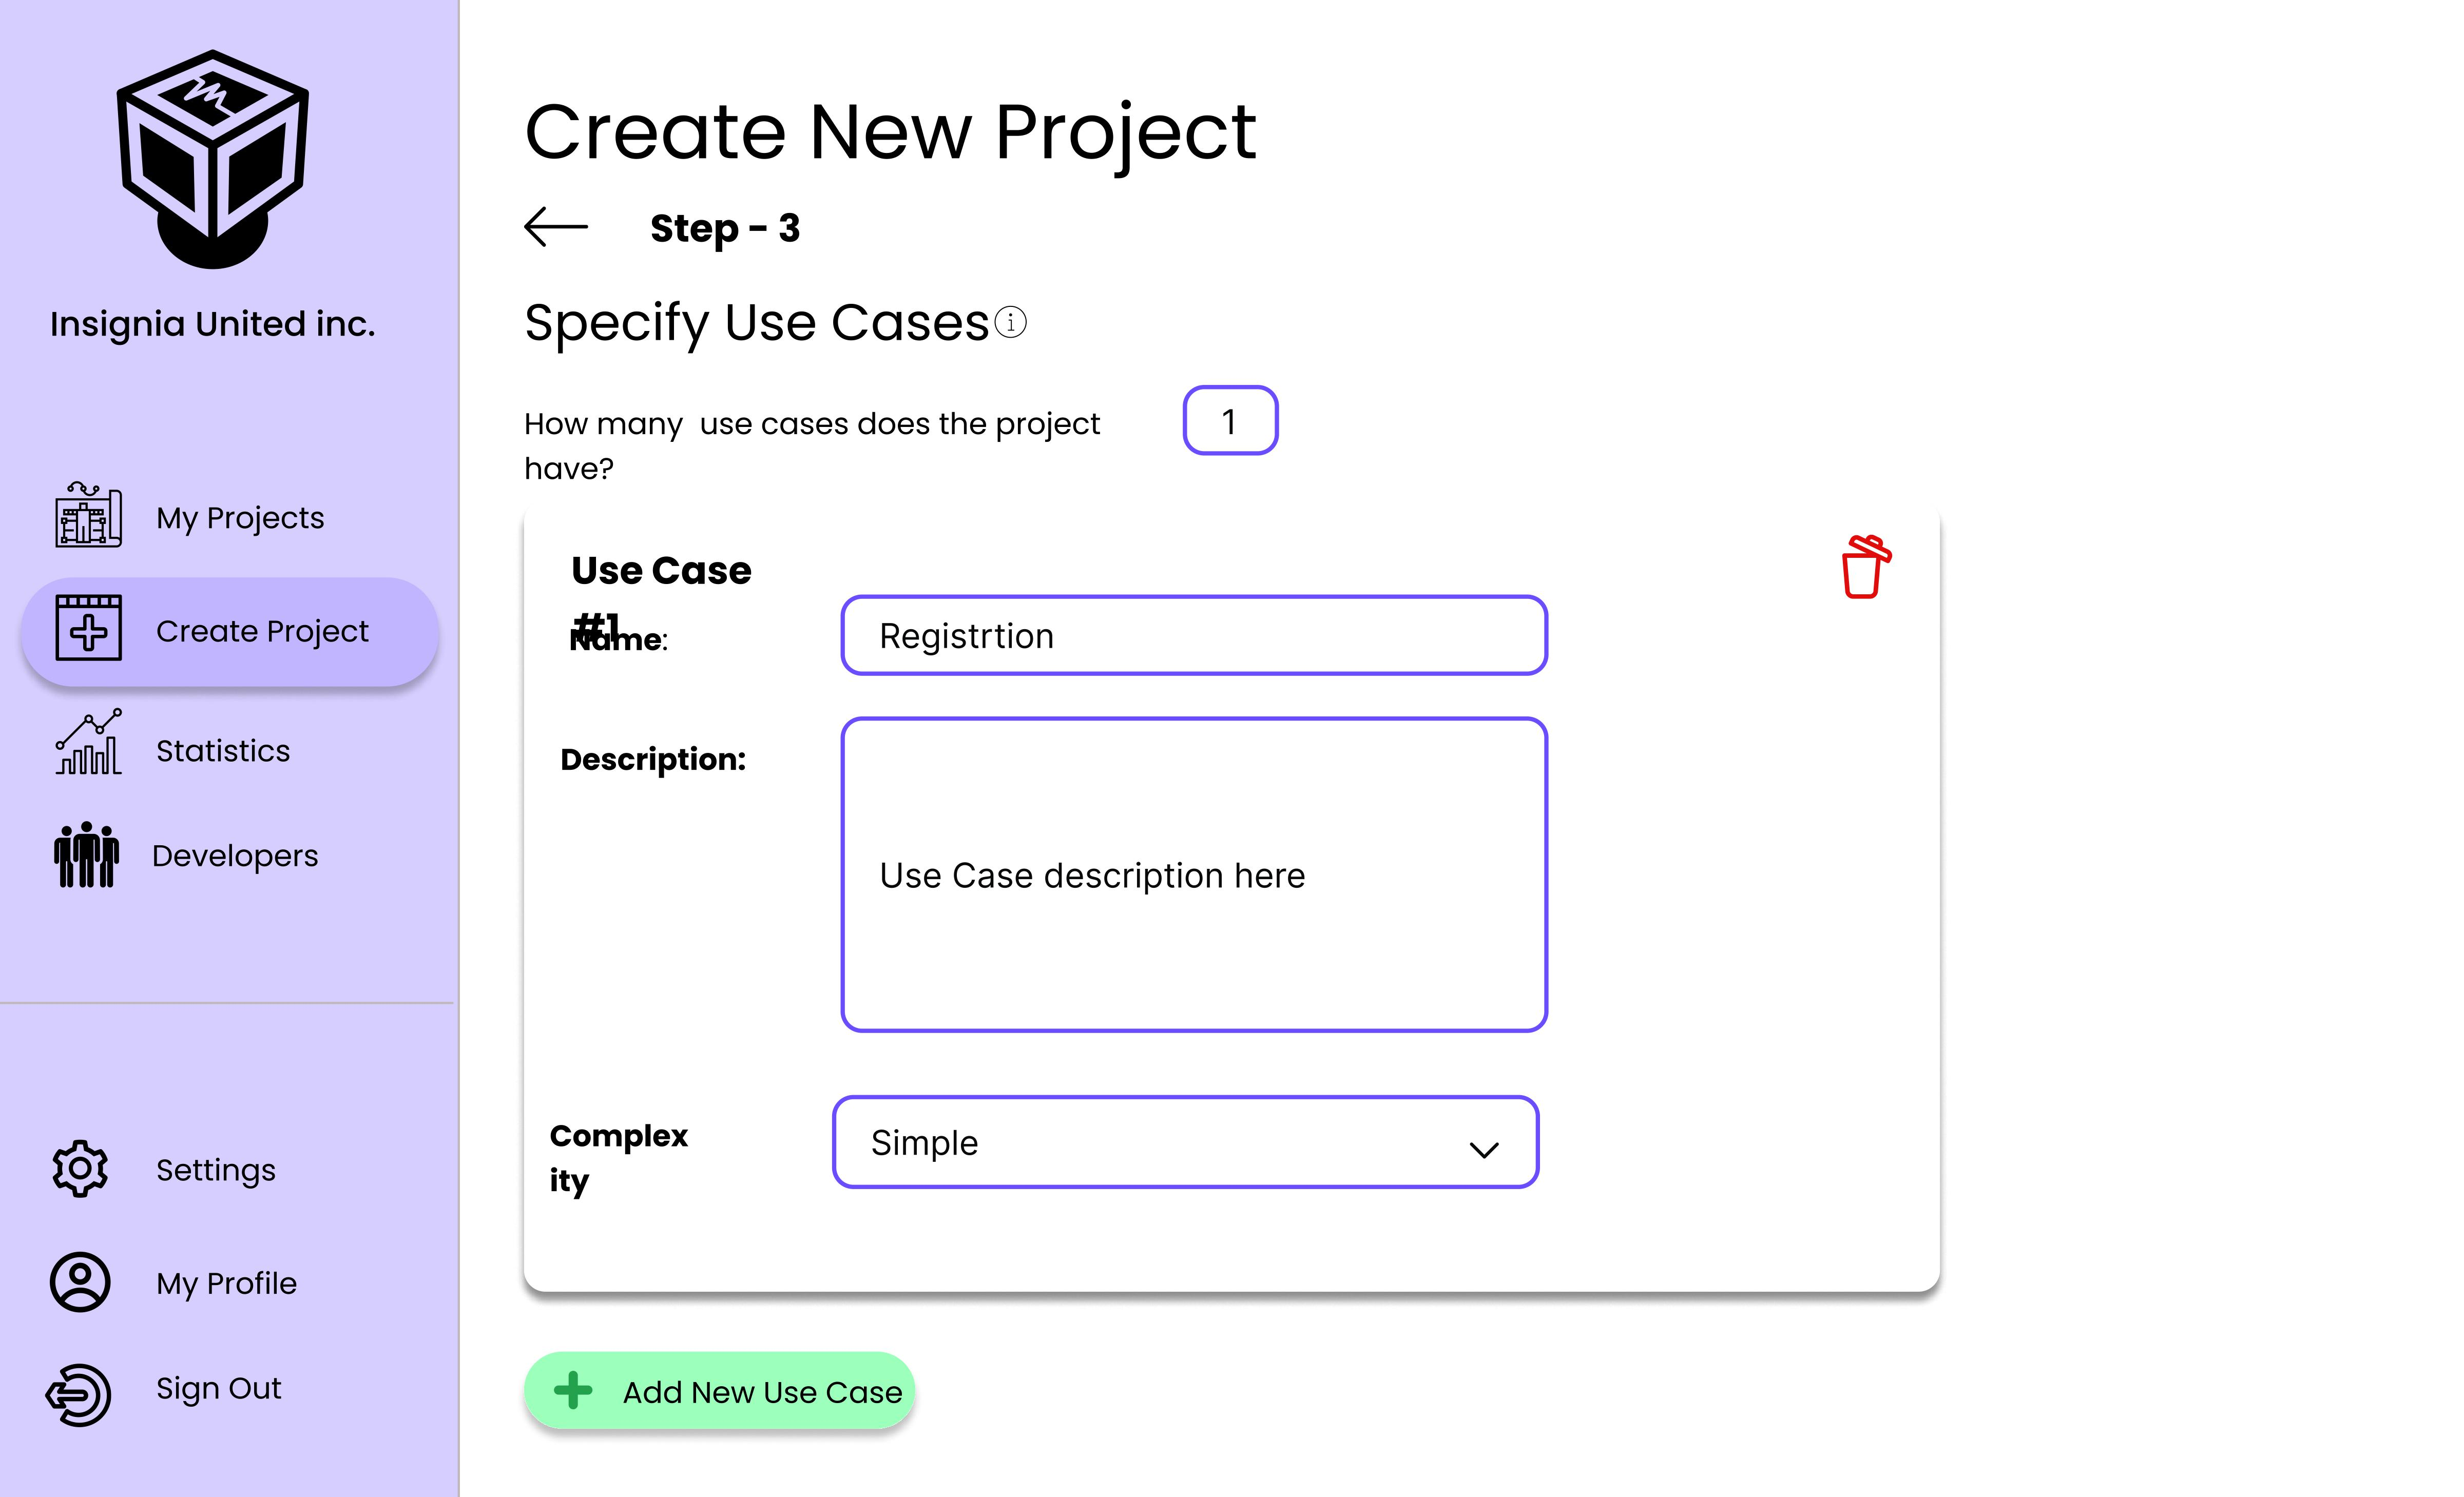
\includegraphics[height=10cm, width=0.9\textwidth]{./images/prototype/0017}
\centering 
\caption{Login Page}
\label{fig:prototype1}
\end{figure}

\begin{figure}[H]
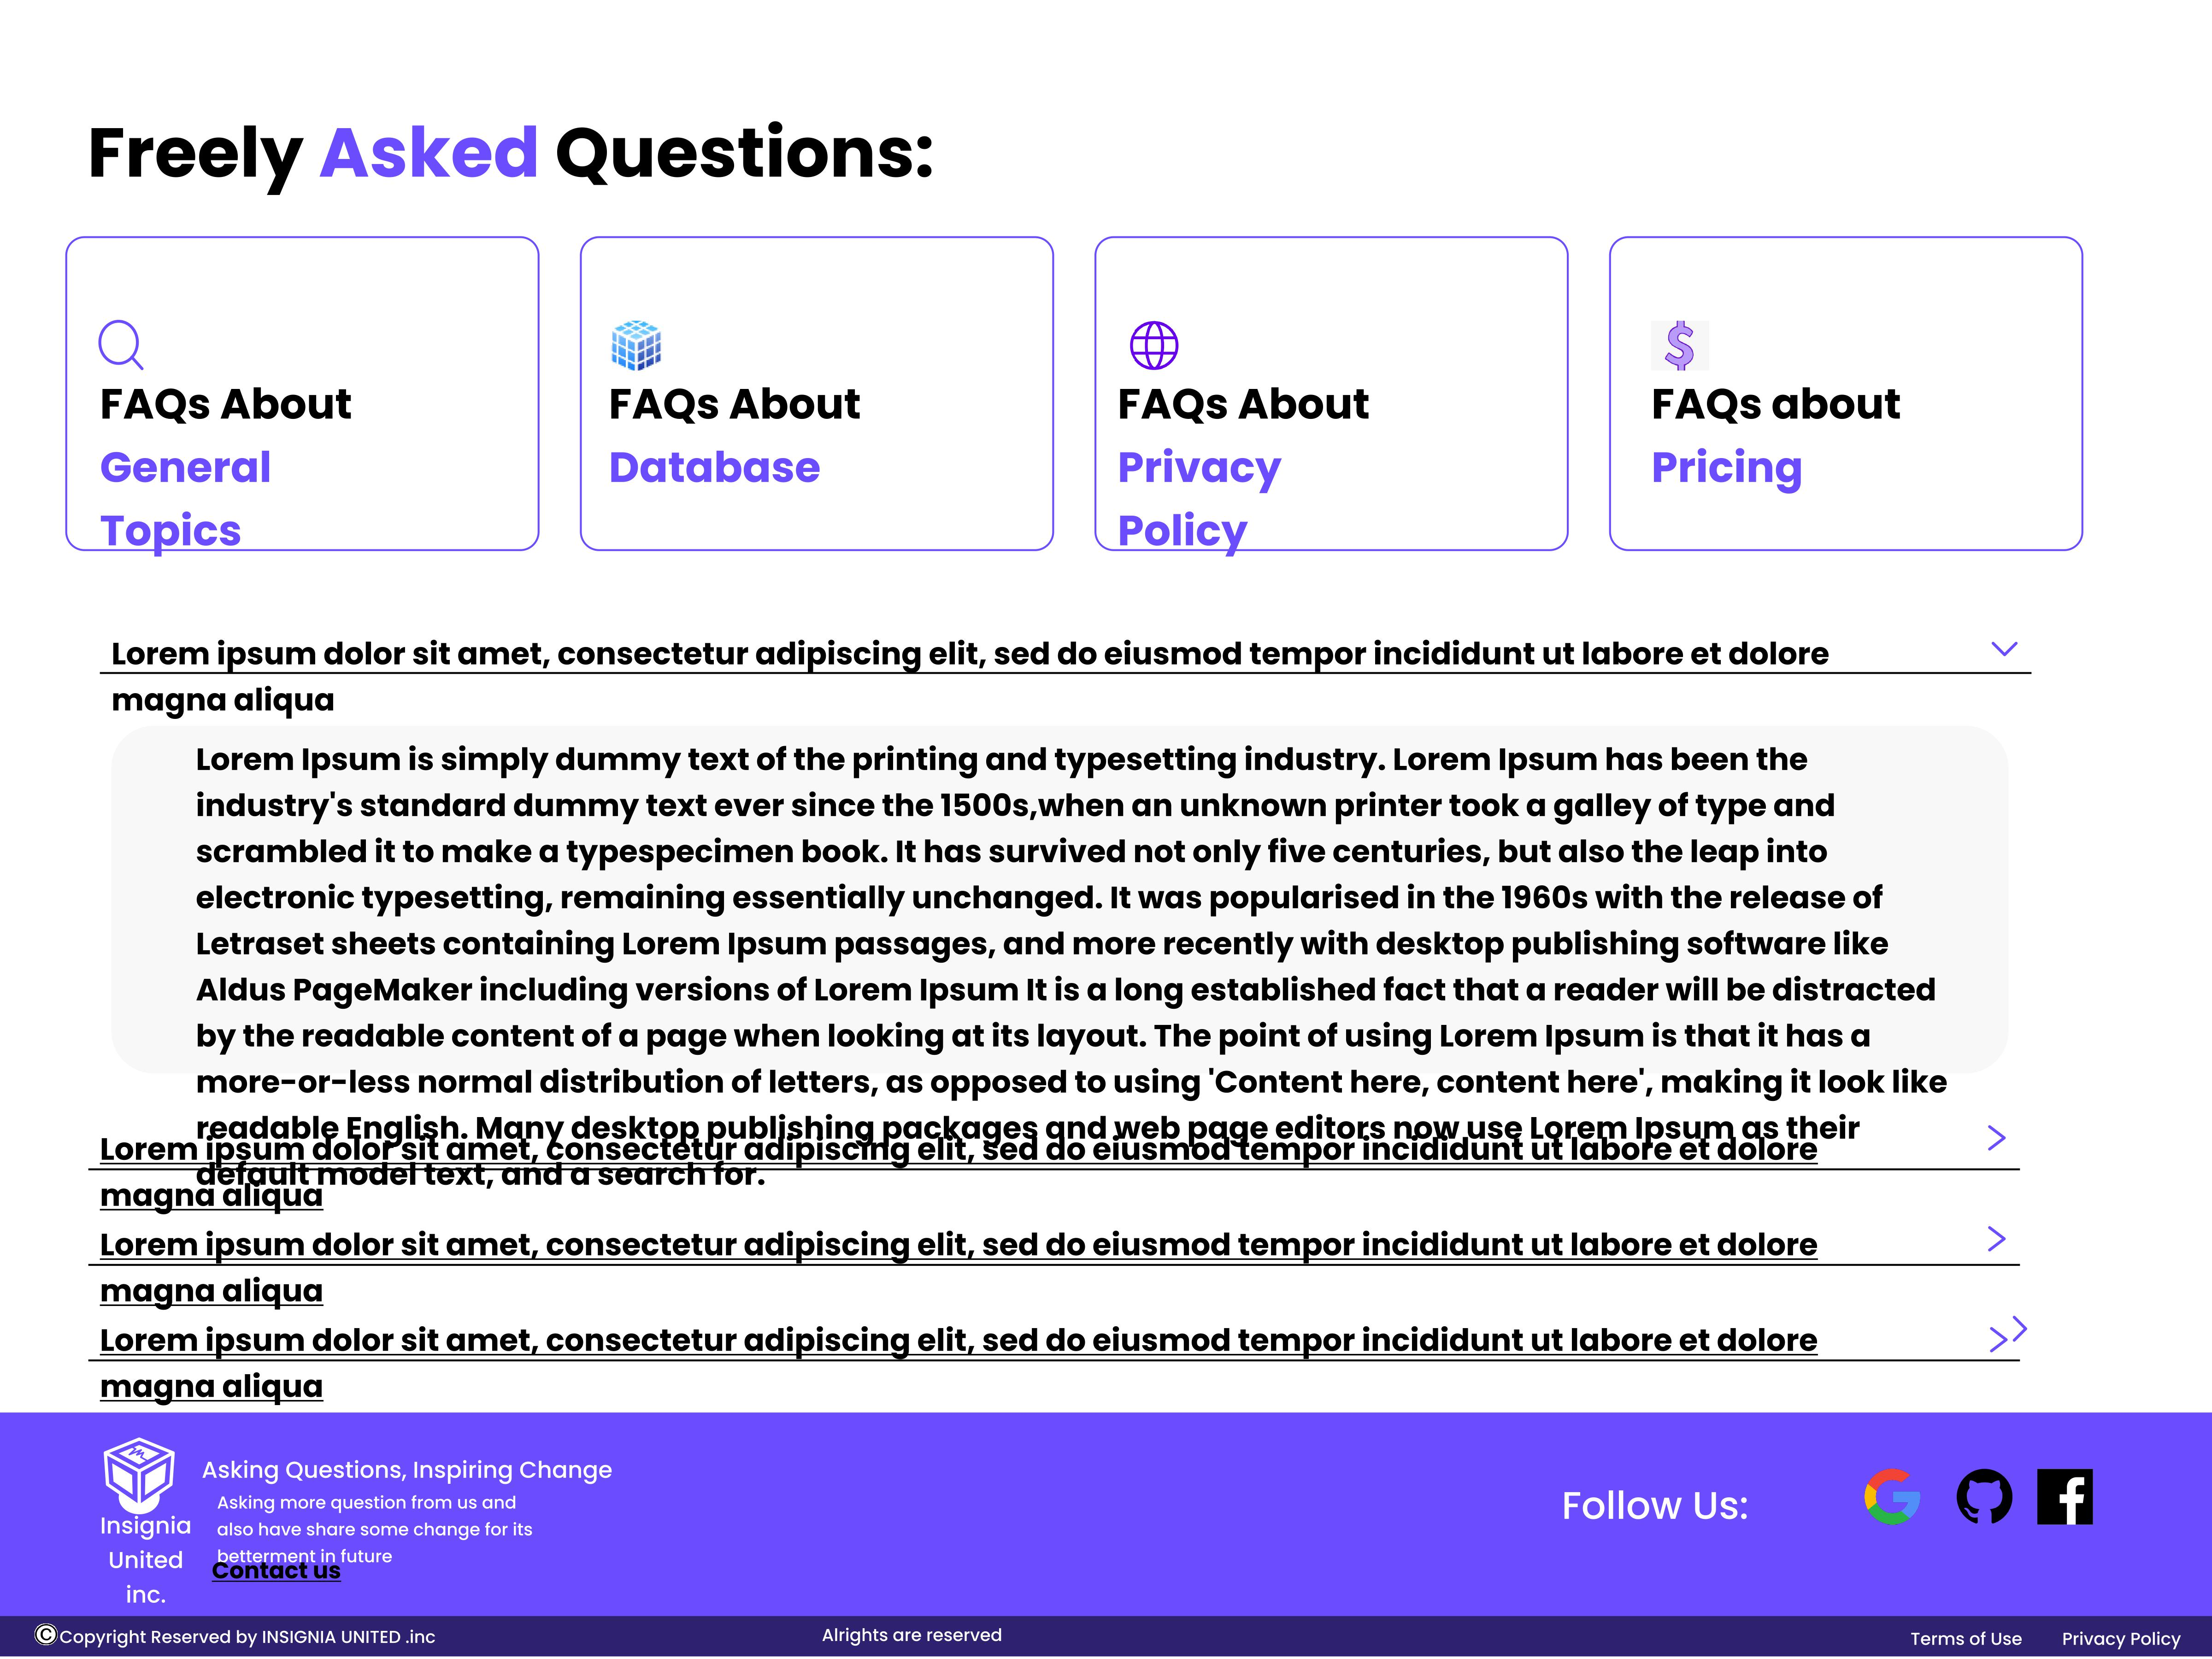
\includegraphics[height=10cm, width=0.9\textwidth]{./images/prototype/0018}
\centering 
\caption{Login Page}
\label{fig:prototype1}

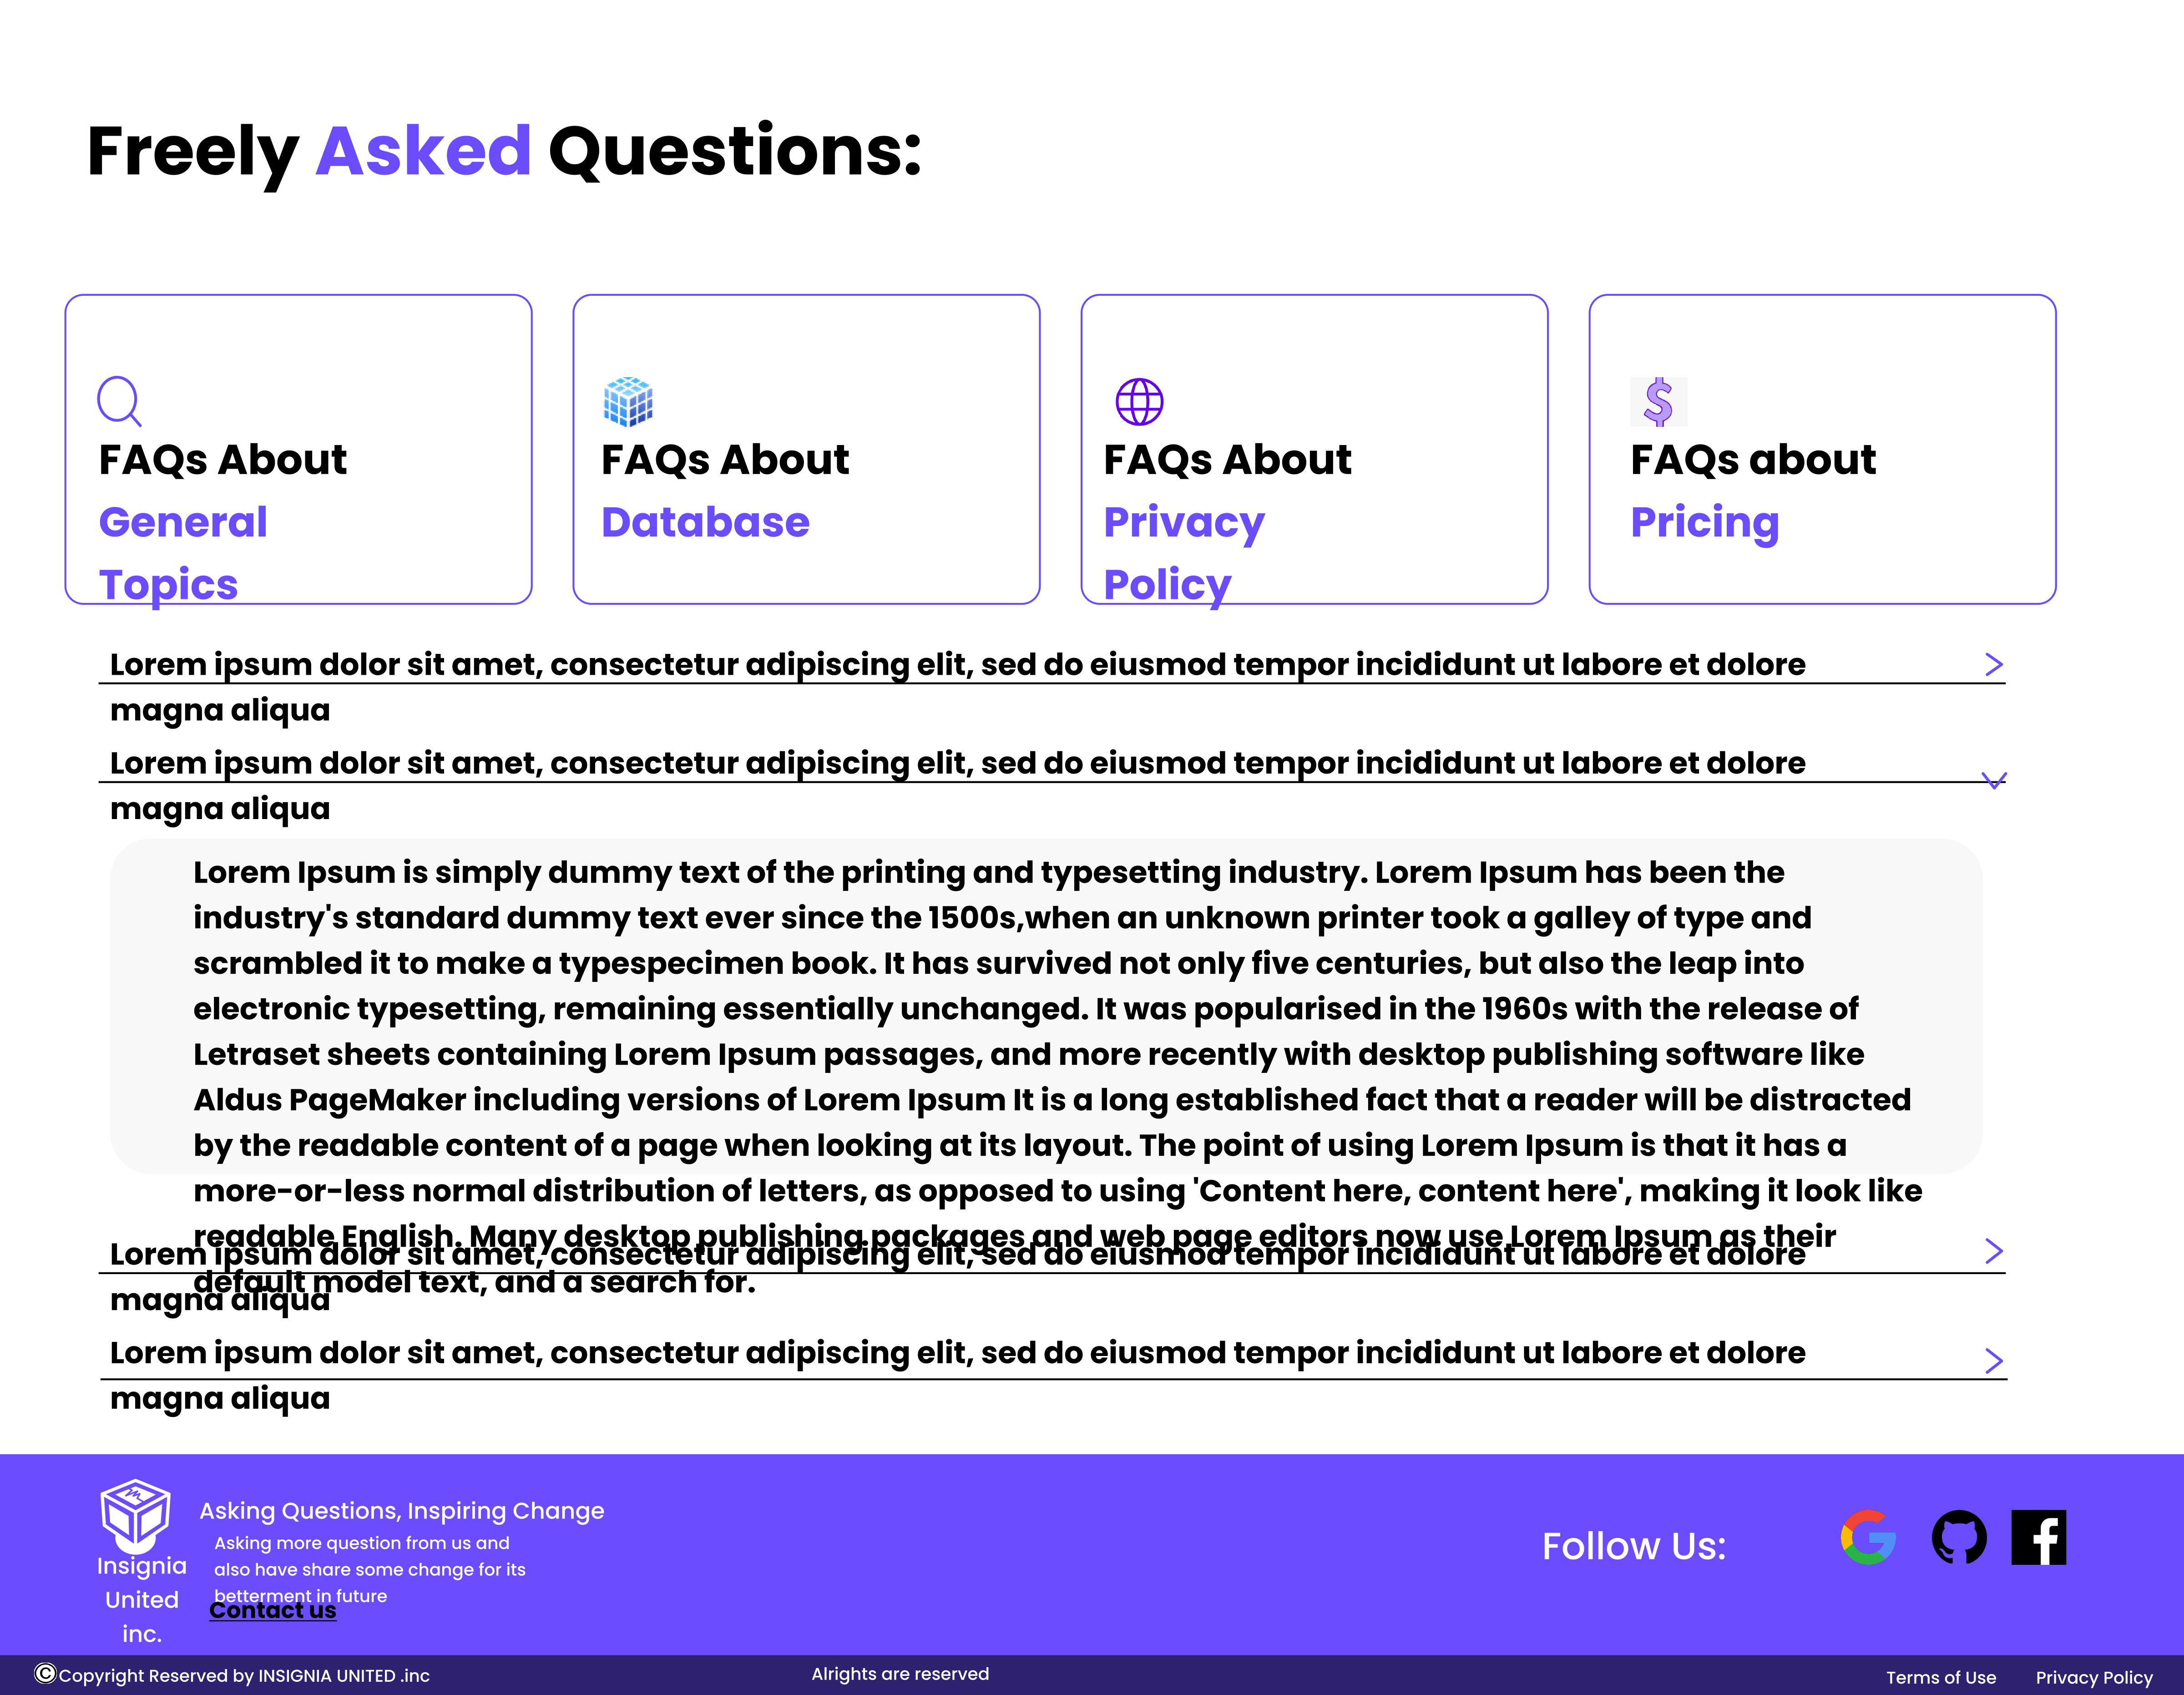
\includegraphics[height=10cm, width=0.9\textwidth]{./images/prototype/0019}
\centering 
\caption{Login Page}
\label{fig:prototype1}
\end{figure}

\begin{figure}[H]
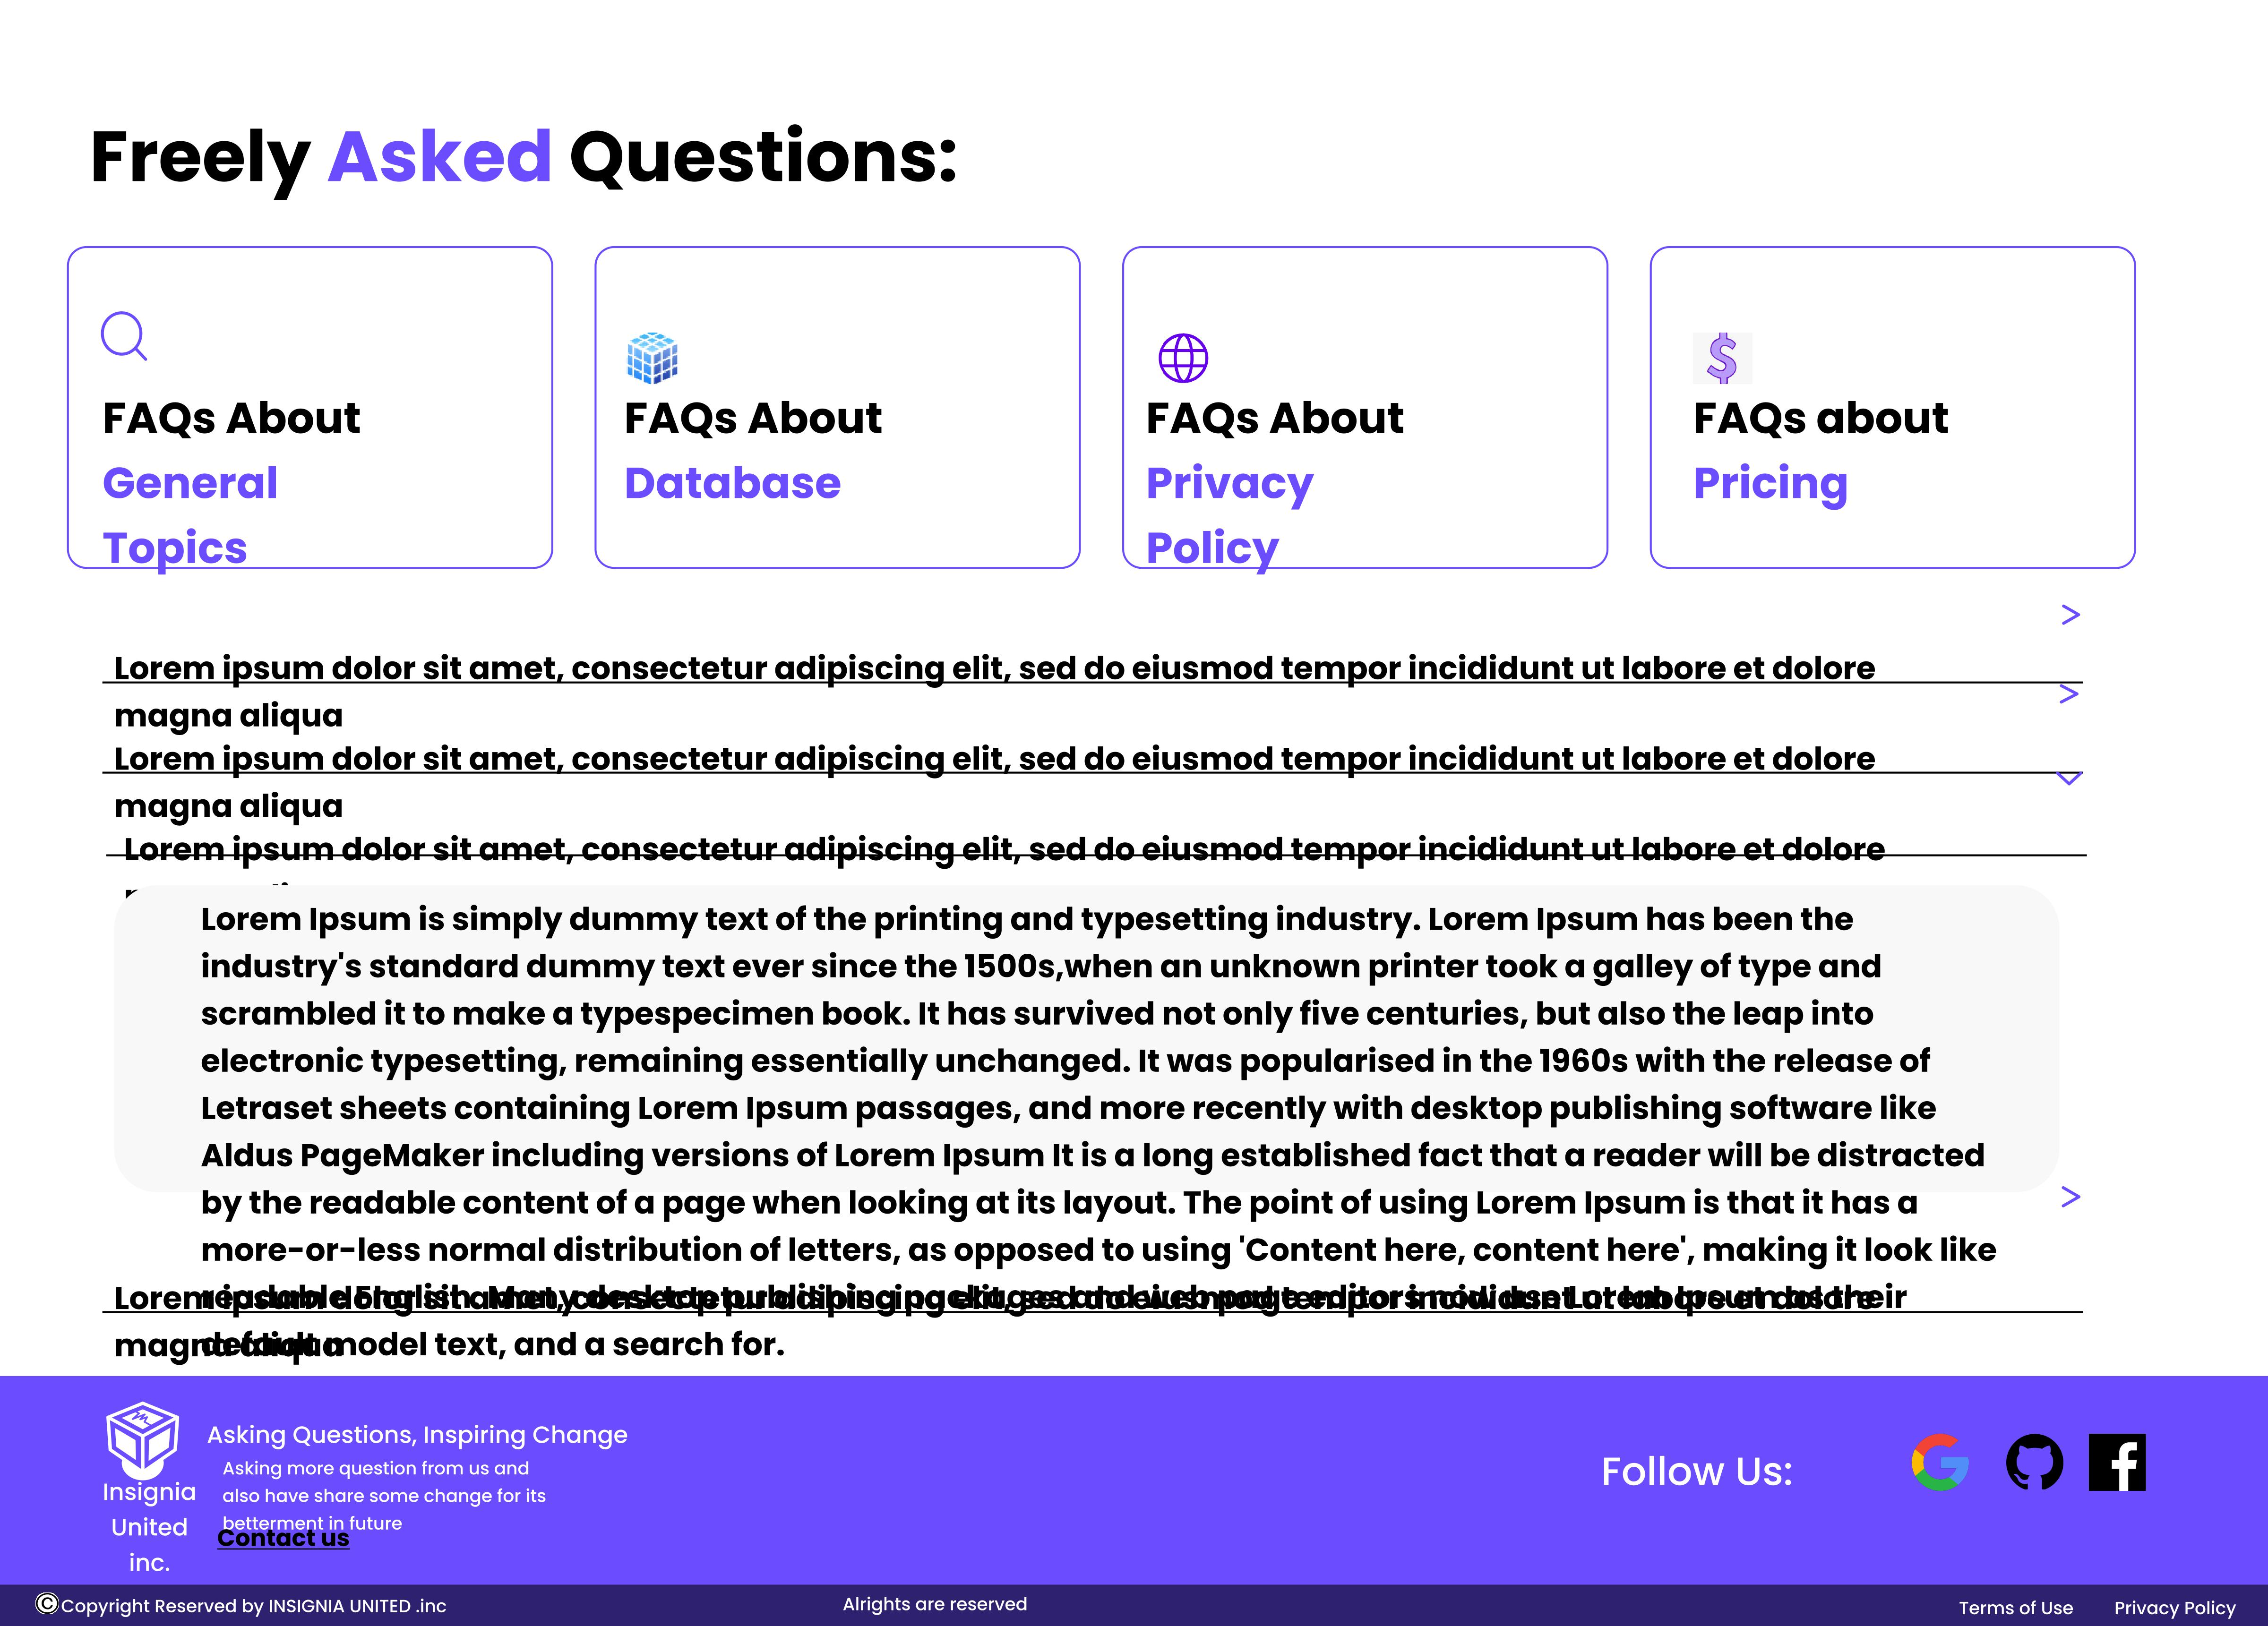
\includegraphics[height=10cm, width=0.9\textwidth]{./images/prototype/0020}
\centering 
\caption{Login Page}
\label{fig:prototype1}

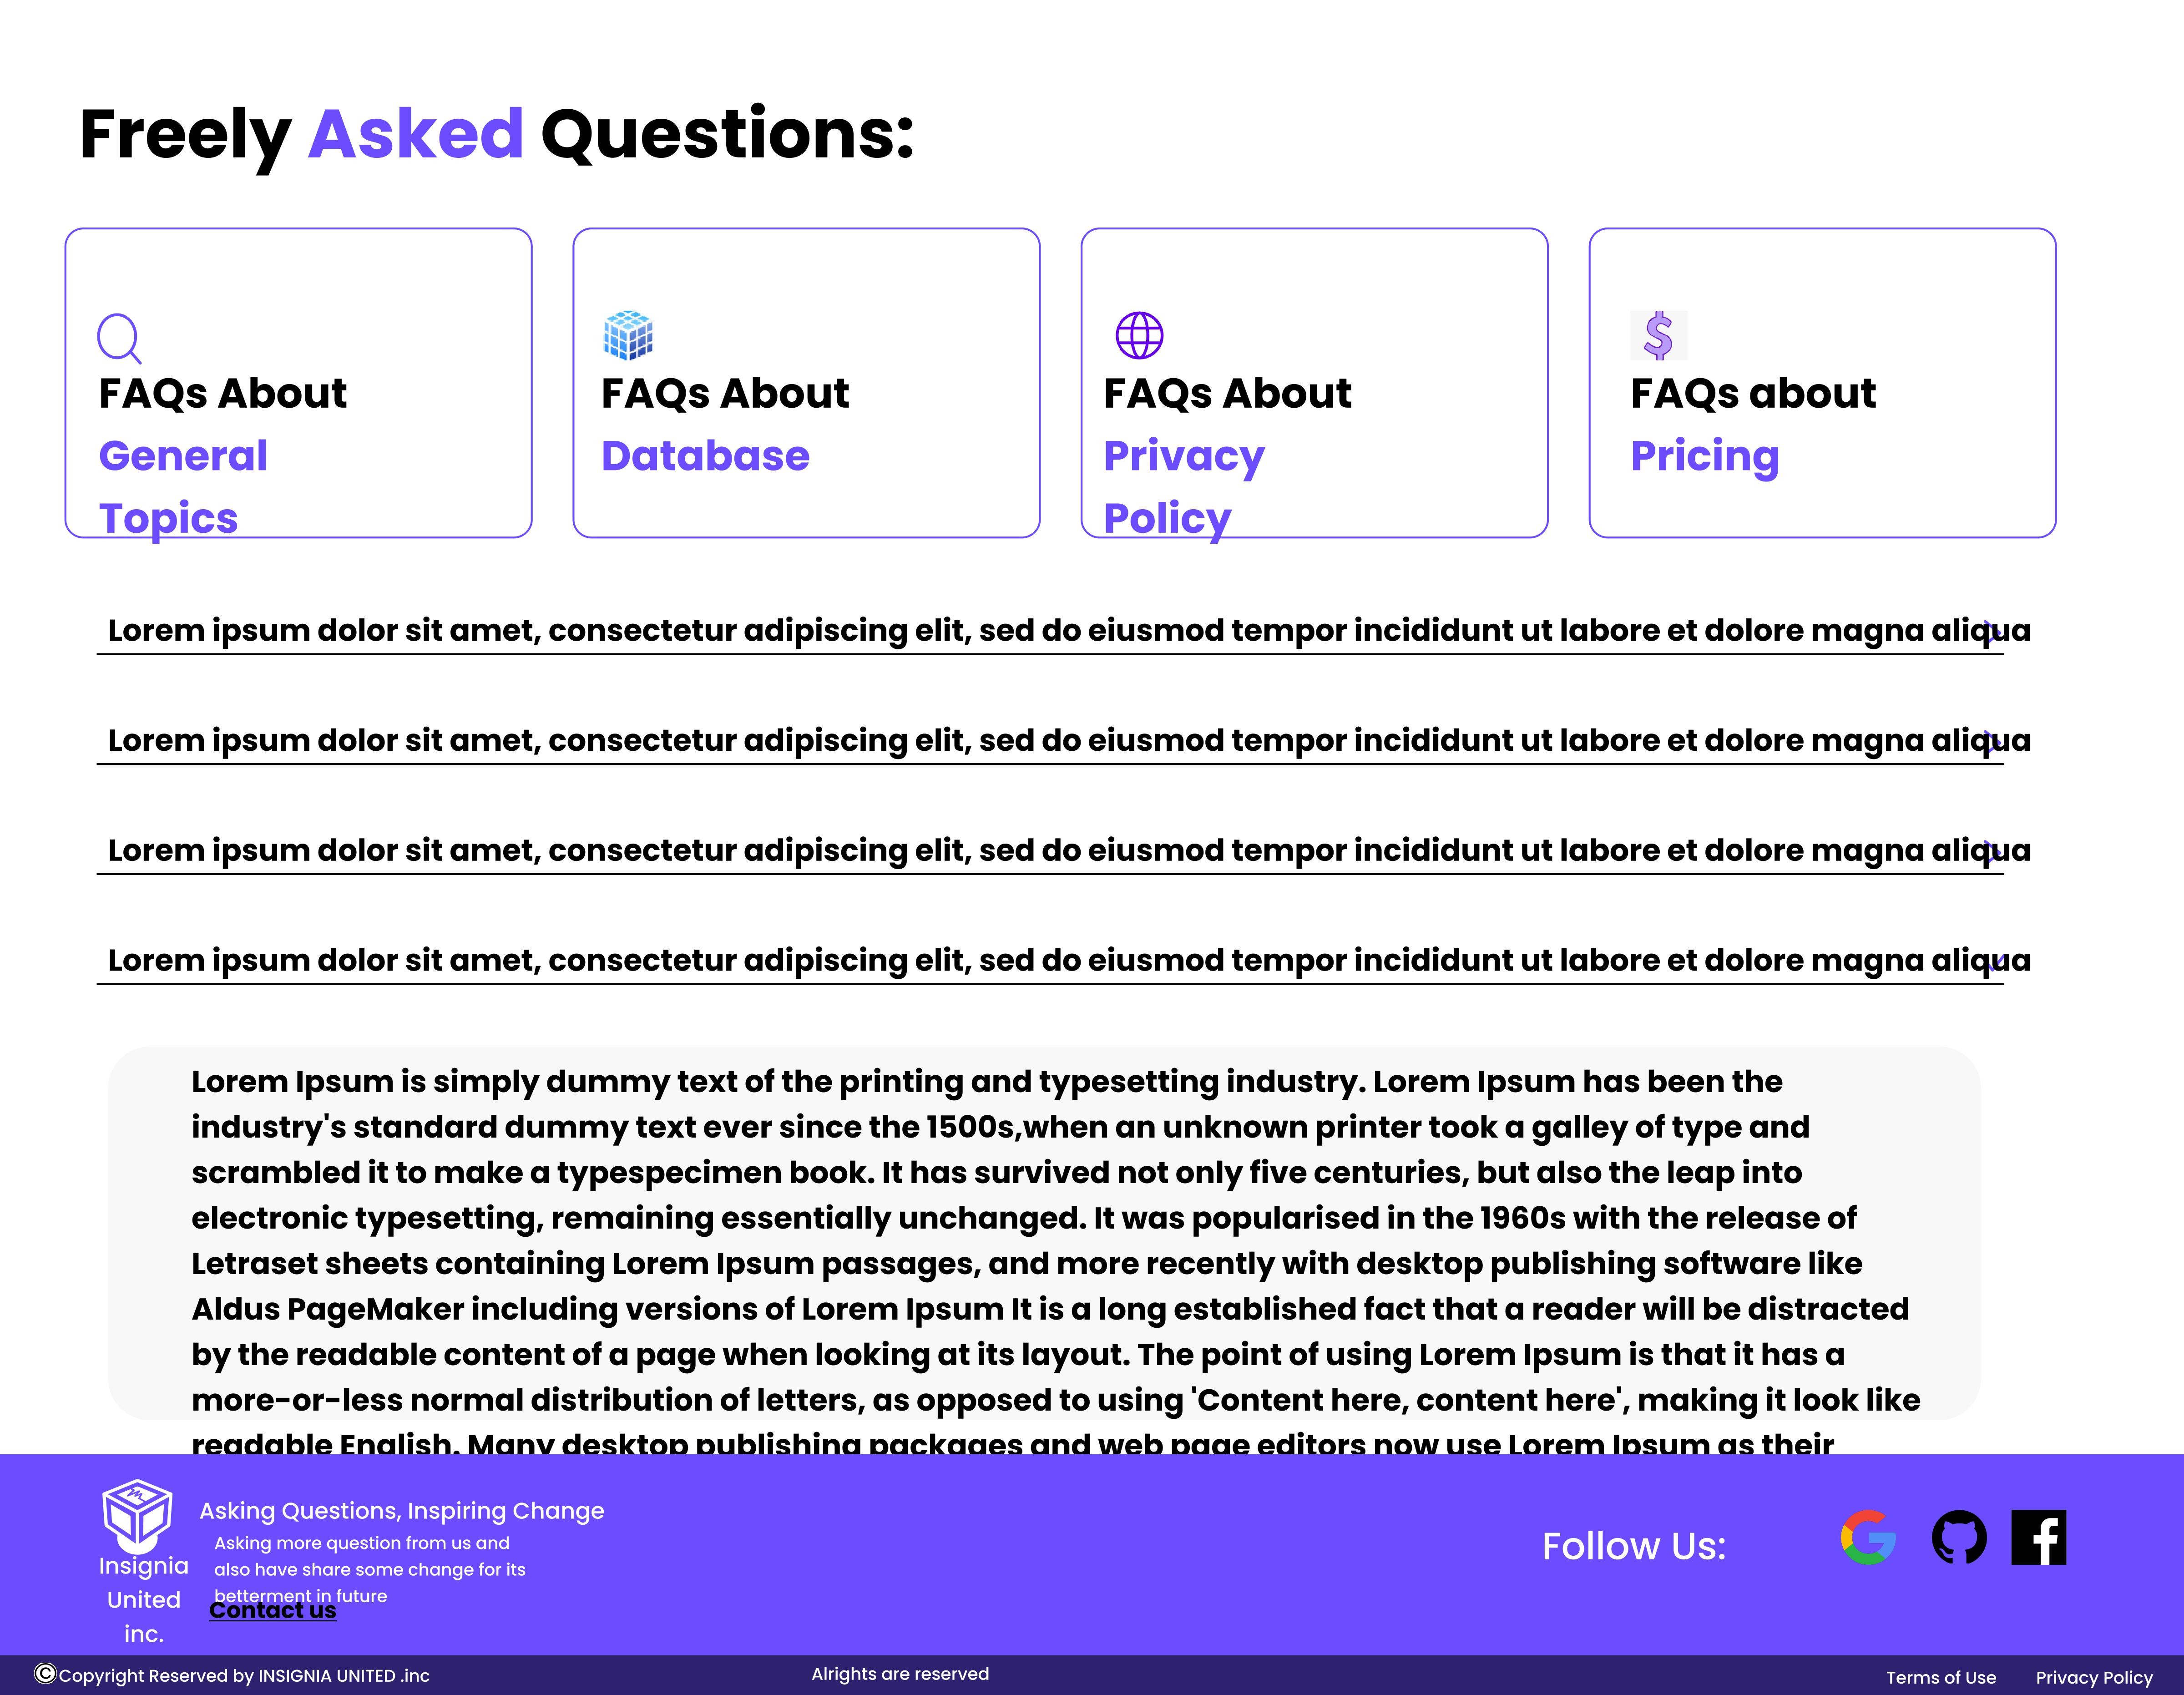
\includegraphics[height=10cm, width=0.9\textwidth]{./images/prototype/0021}
\centering 
\caption{Login Page}
\label{fig:prototype1}

\end{figure}
    
    \pagebreak
    \subsection{Functional Requiremets}
    \newcommand{\splitcell}[2][c]{%
  \begin{tabular}[#1]{@{}c@{}}#2\end{tabular}}
\subsubsection{FR-01: Register}
\begin{center}
  \begin{tabularx}{\textwidth}{|l|X|}
      \hline
      \textbf{ID} & FR-01 \\
      \hline
      \textbf{Name} & Register \\
      \hline
      \textbf{Description} & Register a new user \\
      \hline
      \textbf{Input} & username, password, password\_confirmation, email \\
      \hline
      \textbf{Output} & A new user is created in the database \\
      \hline
      \textbf{Requirements} & Valid username, valid email, password that contains at least 8 characters, password\_confirmation that matches the password \\
      \hline
  \end{tabularx}
\end{center}

\subsubsection{FR-02: Login}
\begin{center}
  \begin{tabularx}{\textwidth}{|l|X|}
      \hline
      \textbf{ID} & FR-02 \\
      \hline
      \textbf{Name} & Login \\
      \hline
      \textbf{Description} & Login to the application \\
      \hline
      \textbf{Input} & username or email, password \\
      \hline
      \textbf{Output} & User is logged in, a JWT token is issued \\
      \hline
      \textbf{Requirements} & Valid username or email, matching password \\
      \hline
  \end{tabularx}
\end{center}

\subsubsection{FR-03: OAuth}
\begin{center}
  \begin{tabularx}{\textwidth}{|l|X|}
      \hline
      \textbf{ID} & FR-03 \\
      \hline
      \textbf{Name} & OAuth \\
      \hline
      \textbf{Description} & Login to the application using OAuth \\
      \hline
      \textbf{Input} & OAuth token \\
      \hline
      \textbf{Output} & User is logged in, a JWT token is issued \\
      \hline
      \textbf{Requirements} & Valid OAuth token \\
      \hline
  \end{tabularx}
\end{center}

\subsubsection{FR-04: Forget Password}
\begin{center}
  \begin{tabularx}{\textwidth}{|l|X|}
      \hline
      \textbf{ID} & FR-04 \\
      \hline
      \textbf{Name} & Forgot password \\
      \hline
      \textbf{Description} & Send an email to the user with a link to reset their password \\
      \hline
      \textbf{Input} & email \\
      \hline
      \textbf{Output} & An email is sent to the user with a link to reset their password \\
      \hline
      \textbf{Requirements} & Valid email \\
      \hline
  \end{tabularx}
\end{center}
\newpage

\subsubsection{FR-05: Reset Password}
\begin{center}
  \begin{tabularx}{\textwidth}{|l|X|}
      \hline
      \textbf{ID} & FR-05 \\
      \hline
      \textbf{Name} & Reset password \\
      \hline
      \textbf{Description} & Reset the user's password \\
      \hline
      \textbf{Input} & token, password, password\_confirmation \\
      \hline
      \textbf{Output} & The user's password is reset \\
      \hline
      \textbf{Requirements} & Valid token, valid password, password\_confirmation that matches the password \\
      \hline
  \end{tabularx}
\end{center}


\subsubsection{FR-06: Confirm Account}
\begin{center}
  \begin{tabularx}{\textwidth}{|l|X|}
      \hline
      \textbf{ID} & FR-06 \\
      \hline
      \textbf{Name} & Confirm account \\
      \hline
      \textbf{Description} & Confirm the user's account \\
      \hline
      \textbf{Input} & token \\
      \hline
      \textbf{Output} & The user's account is confirmed \\
      \hline
      \textbf{Requirements} & Valid token \\
      \hline
  \end{tabularx}
\end{center}

\subsubsection{FR-07: Delete Account}
\begin{center}
  \begin{tabularx}{\textwidth}{|l|X|}
      \hline
      \textbf{ID} & FR-07 \\
      \hline
      \textbf{Name} & Delete account \\
      \hline
      \textbf{Description} & Delete the user's account \\
      \hline
      \textbf{Input} & token \\
      \hline
      \textbf{Output} & The user's account is deleted \\
      \hline
      \textbf{Requirements} & Valid token \\
      \hline
  \end{tabularx}
\end{center}

\subsubsection{FR-08: Create Initial Account}
\begin{center}
  \begin{tabularx}{\textwidth}{|l|X|}
      \hline
      \textbf{ID} & FR-08 \\
      \hline
      \textbf{Name} & Create initial account \\
      \hline
      \textbf{Description} & Create the initial account \\
      \hline
      \textbf{Input} & role \\
      \hline
      \textbf{Output} & A user's information is complete \\
      \hline
      \textbf{Requirements} & A role, either developer or manager \\
      \hline
  \end{tabularx}
\end{center}

\subsubsection{FR-09: Create Initial Account usmanError}
\begin{center}
  \begin{tabularx}{\textwidth}{|l|X|}
      \hline
      \textbf{ID} & FR-09 \\
      \hline
      \textbf{Name} & Create initial account \\
      \hline
      \textbf{Description} & Create the initial account \\
      \hline
      \textbf{Input} & username, password, email \\
      \hline
      \textbf{Output} & The initial account is created \\
      \hline
      \textbf{Requirements} & Valid username, valid email, password that contains at least 8 characters \\
      \hline
  \end{tabularx}
\end{center}

\subsubsection{FR-10: Edit Account Info.}
\begin{center}
  \begin{tabularx}{\textwidth}{|l|X|}
      \hline
      \textbf{ID} & FR-10 \\
      \hline
      \textbf{Name} & Edit account info \\
      \hline
      \textbf{Description} & Edit the user's account info \\
      \hline
      \textbf{Input} & token, username, email \\
      \hline
      \textbf{Output} & The user's account info is updated \\
      \hline
      \textbf{Requirements} & Valid token, valid username, valid email \\
      \hline
  \end{tabularx}
\end{center}

\subsubsection{FR-11: Edit Interface Preference}
\begin{center}
  \begin{tabularx}{\textwidth}{|l|X|}
      \hline
      \textbf{ID} & FR-11 \\
      \hline
      \textbf{Name} & Edit interface preferences \\
      \hline
      \textbf{Description} & Edit the user's interface preferences \\
      \hline
      \textbf{Input} & token, theme, language \\
      \hline
      \textbf{Output} & The user's interface preferences are updated \\
      \hline
      \textbf{Requirements} & Valid token, valid theme, valid language \\
      \hline
  \end{tabularx}
\end{center}

\subsubsection{FR-12: Create Project}
\begin{center}
  \begin{tabularx}{\textwidth}{|l|X|}
      \hline
      \textbf{ID} & FR-12 \\
      \hline
      \textbf{Name} & Create Project \\
      \hline
      \textbf{Description} & The manager creates a fresh project \\
      \hline
      \textbf{Input} & use cases (file/forms), add developers(optional), project name, technology \\
      \hline
      \textbf{Output} & A new project is created in the database with the ID of its manager \\
      \hline
      \textbf{Requirements} & Use cases, name, technology name \\
      \hline
  \end{tabularx}
\end{center}

\subsubsection{FR-13: Edit Project}
\begin{center}
  \begin{tabularx}{\textwidth}{|l|X|}
      \hline
      \textbf{ID} & FR-13 \\
      \hline
      \textbf{Name} & Edit Project \\
      \hline
      \textbf{Description} & The manager edits an existing project \\
      \hline
      \textbf{Input} & use cases (file/forms), project name, technology, (all optional), project ID(needed) \\
      \hline
      \textbf{Output} & The referred project is  \\
      \hline
      \textbf{Requirements} & Use cases, name, technology name, manager logged in, project exists \\
      \hline
  \end{tabularx}
\end{center}

\subsubsection{FR-14: Delete Project}
\begin{center}
  \begin{tabularx}{\textwidth}{|l|X|}
      \hline
      \textbf{ID} & FR-14 \\
      \hline
      \textbf{Name} & Delete Project \\
      \hline
      \textbf{Description} & The manager removes an existing project from database \\
      \hline
      \textbf{Input} & Manager clicks on delete project and clicks Yes \\
      \hline
      \textbf{Output} & The referred project is removed from database \\
      \hline
      \textbf{Requirements} & Project ID, manager logged in \\
      \hline
  \end{tabularx}
\end{center}

\subsubsection{FR-15: Add Developer}
\begin{center}
  \begin{tabularx}{\textwidth}{|l|X|}
      \hline
      \textbf{ID} & FR-15 \\
      \hline
      \textbf{Name} & Add Developer \\
      \hline
      \textbf{Description} & The manager assigns a developer to the project \\
      \hline
      \textbf{Input} & Manager clicks on add new developer and types developer's username \\
      \hline
      \textbf{Output} & A new developer is added to projects developer's list \\
      \hline
      \textbf{Requirements} & Project ID, manager logged in, developer username \\
      \hline
  \end{tabularx}
\end{center}

\subsubsection{FR-16: Remove Developer}
\begin{center}
  \begin{tabularx}{\textwidth}{|l|X|}
      \hline
      \textbf{ID} & FR-16 \\
      \hline
      \textbf{Name} & Remove Developer \\
      \hline
      \textbf{Description} & The manager removes a developer from the project \\
      \hline
      \textbf{Input} & Manager goes into developers list and clicks remove button and then clicks Yes \\
      \hline
      \textbf{Output} & The developer is removed from the project's developers list \\
      \hline
      \textbf{Requirements} & Project ID, manager logged in, developer username \\
      \hline
  \end{tabularx}
\end{center}

\subsubsection{FR-17: Edit Developer Permission}
\begin{center}
  \begin{tabularx}{\textwidth}{|l|X|}
      \hline
      \textbf{ID} & FR-17 \\
      \hline
      \textbf{Name} & Edit Developer Permissions \\
      \hline
      \textbf{Description} & Manager changes a developer's access level to the project \\
      \hline
      \textbf{Input} & Manager goes tp developers list and clicks on change role on a developer. They then choose either View or Edit \\
      \hline
      \textbf{Output} & Project permissions are edited \\
      \hline
      \textbf{Requirements} & Project ID, Developer ID, Permission type, manager logged in \\
      \hline
  \end{tabularx}
\end{center}

\subsubsection{FR-18: Calculate UCP}
\begin{center}
  \begin{tabularx}{\textwidth}{|l|X|}
      \hline
      \textbf{ID} & FR-18 \\
      \hline
      \textbf{Name} & Calculate UCP \\
      \hline
      \textbf{Description} & Get UCP estimation of project using use cases \\
      \hline
      \textbf{Input} & Use Cases, environmental factors, technical factors \\
      \hline
      \textbf{Output} & An integer representing the UCP estimation in man hours \\
      \hline
      \textbf{Requirements} & manager logged in, use at least 2 cases are entered \\
      \hline
  \end{tabularx}
\end{center}

\subsubsection{FR-19: Get Machine Learning Estimate}
\begin{center}
  \begin{tabularx}{\textwidth}{|l|X|}
      \hline
      \textbf{ID} & FR-19 \\
      \hline
      \textbf{Name} & Get Machine Learning Estimate \\
      \hline
      \textbf{Description} & Calculate estimate using machine learning model \\
      \hline
      \textbf{Input} & Use Cases, environmental factors, technical factors \\
      \hline
      \textbf{Output} & An integer representing the machine learning estimation in man hours \\
      \hline
      \textbf{Requirements} & manager logged in, use at least 2 cases are entered \\
      \hline
  \end{tabularx}
\end{center}

\subsubsection{FR-20: Start Manual Estimation Round}
\begin{center}
  \begin{tabularx}{\textwidth}{|l|X|}
      \hline
      \textbf{ID} & FR-20 \\
      \hline
      \textbf{Name} & Start Manual Estimation Round \\
      \hline
      \textbf{Description} & Create an empty round in current project \\
      \hline
      \textbf{Input} & Manager clicks on start manual estimation \\
      \hline
      \textbf{Output} & Empty round is created in database for current project \\
      \hline
      \textbf{Requirements} & Manager logged in, project exists, project has at least two use case, at least one developer assigned to project \\
      \hline
  \end{tabularx}
\end{center}

\subsubsection{FR-21: End Round}
\begin{center}
  \begin{tabularx}{\textwidth}{|l|X|}
      \hline
      \textbf{ID} & FR-21 \\
      \hline
      \textbf{Name} & End Round \\
      \hline
      \textbf{Description} & End current round, locking in all estimates given so far \\
      \hline
      \textbf{Input} & Manager clicks end round \\
      \hline
      \textbf{Output} & Round length is increased by one and all estimates are locked in \\
      \hline
      \textbf{Requirements} & Round exists, manager logged in, at least one estimate is made \\
      \hline
  \end{tabularx}
\end{center}

\subsubsection{FR-22: Clear Round}
\begin{center}
  \begin{tabularx}{\textwidth}{|l|X|}
      \hline
      \textbf{ID} & FR-22 \\
      \hline
      \textbf{Name} & Clear Round \\
      \hline
      \textbf{Description} & Clear current round's estimates \\
      \hline
      \textbf{Input} & Manager clicks on clear round \\
      \hline
      \textbf{Output} & All of estimates made for this round are deleted \\
      \hline
      \textbf{Requirements} & Round exists, manager logged in, at least one estimate is made \\
      \hline
  \end{tabularx}
\end{center}

\subsubsection{FR-23: Calculate Round Average}
\begin{center}
  \begin{tabularx}{\textwidth}{|l|X|}
      \hline
      \textbf{ID} & FR-23 \\
      \hline
      \textbf{Name} & Calculate Round Average \\
      \hline
      \textbf{Description} & Process all given estimates and calculate average \\
      \hline
      \textbf{Input} & A round is finished \\
      \hline
      \textbf{Output} & Average is calculated and stored in database for current round \\
      \hline
      \textbf{Requirements} & Round exists, manager logged in, at least one estimate is made \\
      \hline
  \end{tabularx}
\end{center}

\subsubsection{FR-24: Finalize Manual Estimation}
\begin{center}
  \begin{tabularx}{\textwidth}{|l|X|}
      \hline
      \textbf{ID} & FR-24 \\
      \hline
      \textbf{Name} & Finalize Manual Estimation \\
      \hline
      \textbf{Description} & Multiple rounds are finished and the team has agreed on a final estimate \\
      \hline
      \textbf{Input} & Manager clicks on finalize button \\
      \hline
      \textbf{Output} & Manual estimation is calculated and stored in database for current round \\
      \hline
      \textbf{Requirements} & Al least one round finished, manager logged in \\
      \hline
  \end{tabularx}
\end{center}

\subsubsection{FR-25: AllEstimate Bar Chart}
\begin{center}
  \begin{tabularx}{\textwidth}{|l|X|}
      \hline
      \textbf{ID} & FR-25 \\
      \hline
      \textbf{Name} & All Estimate Bar Chart \\
      \hline
      \textbf{Description} & Generate a bar chart comparing all types of estimates \\
      \hline
      \textbf{Input} & UCP estimate, manual estimate, ML estimate \\
      \hline
      \textbf{Output} & A bar chart is generated \\
      \hline
      \textbf{Requirements} & At least one type of estimate calculated \\
      \hline
  \end{tabularx}
\end{center}

\subsubsection{FR-26: All Manual Estimate Rounds' Line Chart}
\begin{center}
  \begin{tabularx}{\textwidth}{|l|X|}
      \hline
      \textbf{ID} & FR-26 \\
      \hline
      \textbf{Name} & All Manual Estimate Rounds' Line Chart \\
      \hline
      \textbf{Description} & A line chart of all rounds' estimates generated overtime \\
      \hline
      \textbf{Input} & All rounds' averages \\
      \hline
      \textbf{Output} & A line chart is generated \\
      \hline
      \textbf{Requirements} & At least one round has been finished \\
      \hline
  \end{tabularx}
\end{center}

\subsubsection{FR-27: All Manual Estimate Rounds' Bar Chart usman ERROR}
\begin{center}
  \begin{tabularx}{\textwidth}{|l|X|}
      \hline
      \textbf{ID} & FR-27 \\
      \hline
      \textbf{Name} & All Manual Estimate Rounds' Bar Chart \\
      \hline
      \textbf{Description} & A bar chart with showing the progressing of manual estimation rounds while highlighting each developer's estimate \\
      \hline
      \textbf{Input} & round estimates , developers' estimates \\
      \hline
      \textbf{Output} & A bar chart is generated \\
      \hline
      \textbf{Requirements} & At least one round has been finished \\
      \hline
  \end{tabularx}
\end{center}

\subsubsection{FR-28: All Machine Learning Estimates Line Chart}
\begin{center}
  \begin{tabularx}{\textwidth}{|l|X|}
      \hline
      \textbf{ID} & FR-28 \\
      \hline
      \textbf{Name} & All Machine Learning Estimates Line Chart \\
      \hline
      \textbf{Description} & Generate a line chart of all machine learning estimates so far \\
      \hline
      \textbf{Input} & Machine learning estimates \\
      \hline
      \textbf{Output} & A line chart is generated \\
      \hline
      \textbf{Requirements} & At least one ML estimate calculated \\
      \hline
  \end{tabularx}
\end{center}

\subsubsection{FR-29: Pie Chart of Use Cases Weight}
\begin{center}
  \begin{tabularx}{\textwidth}{|l|X|}
      \hline
      \textbf{ID} & FR-29 \\
      \hline
      \textbf{Name} & Pie Chart of Use Cases Weight \\
      \hline
      \textbf{Description} & A pie chart showcasing the most important use cases \\
      \hline
      \textbf{Input} & Use cases \\
      \hline
      \textbf{Output} & A pie chart is generated \\
      \hline
      \textbf{Requirements} & At least two use cases are entered \\
      \hline
  \end{tabularx}
\end{center}

\subsubsection{FR-30: Template of FR}
\begin{center}
  \begin{tabularx}{\textwidth}{|l|X|}
      \hline
      \textbf{ID} & FR-30 \\
      \hline
      \textbf{Name} &  \\
      \hline
      \textbf{Description} &  \\
      \hline
      \textbf{Input} &  \\
      \hline
      \textbf{Output} &  \\
      \hline
      \textbf{Requirements} &  \\
      \hline
  \end{tabularx}
\end{center}
    


\subsection{User Characteristics}
\subsection*{Application User}
After the compeletion of project, application user will able to estimate the budget as well as effort of the new project and later on it will be save for the future if any similar project will be arrive they make sure the effort of that type of software will be this.
Application User will easily entertain their client with the almost accurate budget. 
\subsubsection{Constraint}
The application need an internet access it will not work without internet access.
\subsubsection{Assumptions and dependencies}
\begin{center}
    \begin{itemize}
        \item This application will target the Managers of the Software Associations to find the almost actual effort as well as budget of the upcoming project.
        \item User should know the basic knowledge of the system.
    \end{itemize}
\end{center}
\subsection{Non Functional Requirements}
\subsubsection{Usability}
Usability of the system is high because it is easy to use. Names of choices are very clear and according to their functionality. Its interface is not difficult as user can understand
everything clearly and use its functionality without any confusion.  
\subsubsection{Maintainability}
Maintainability is probability that a failed component or system will be restored or repaired to a specific condition within specificed period or time when maintenance is performed in acoordance with prescribed procedures. So, System will be developed module wise so Maintainability will be achieved by architecture.
\subsubsection{Reusability}
The application designed so that its code can be reused in other application similar to this application and as well as in other applications.
\subsubsection{Response Time}
Response time depends on the speed of internet of user. Higher the spped of internet higher will be the reponse time.
